%\documentclass[10pt, oneside, openany]{book}
\RequirePackage{ifpdf}
\ifpdf
	\documentclass[twoside, justified, notoc, nobib, 
	%openany, 
	nohyper]{tufte-book}
\else
	\documentclass[twoside, justified, notoc, nobib, 
	%openany, 
	nols,nohyper]{tufte-book}
  % PSTricks run
  \usepackage{pstricks}
  \usepackage{pstricks-add}
\fi
%\usepackage{auto-pst-pdf}


%%%%%%%%%%%%%%%%%%%%%%%%%%%%%%%%%%%%%%%%%%%%%%%%%%%%%%%%%%%%%%%%%%%%%%%%%
% Book metadata
%%%%%%%%%%%%%%%%%%%%%%%%%%%%%%%%%%%%%%%%%%%%%%%%%%%%%%%%%%%%%%%%%%%%%%%%%
\title{Neural bases of variable binding in symbolic representations}
\author{Mart\'in P\'erez-Guevara}
\publisher{Unicog lab}

%\usepackage{sidenotes}
\usepackage[orig,french]{isodate}
\usepackage{amsmath,amssymb,amsfonts,amsbsy,amsthm}
\usepackage{algorithm}
\usepackage{algorithmic}
\usepackage{float}
\usepackage[USenglish]{babel} % English language/hyphenation

\usepackage{multirow}
\usepackage{wrapfig}
\usepackage{minitoc}
\usepackage{framed}
\usepackage{upgreek}
\usepackage[absolute]{textpos}
\usepackage{comment}
\usepackage{fancyvrb}
\usepackage{rotating}
\usepackage{calc}
\usepackage{tikz} % Required for drawing custom shapes
\usepackage{graphicx} % Required for including pictures
\usepackage{xcolor, color, colortbl} % Required for specifying colors by name
\usepackage{setspace}
\usepackage{mdframed}
\usepackage{bookmark}
\usepackage{flafter}


\usepackage{natbib}
\usepackage{hyperref}
\usepackage{url}

\setcitestyle{square,numbers}
%\setcitestyle{authoryear}


\newcommand*{\horzbar}{\rule[.6ex]{2.5ex}{0.5pt}}
\newcommand*{\vertbar}{\rule[-1ex]{0.5pt}{2.5ex}}

\usepackage{array}
\newcolumntype{L}[1]{>{\raggedright\let\newline\\\arraybackslash\hspace{0pt}}m{#1}}
\newcolumntype{C}[1]{>{\centering\let\newline\\\arraybackslash\hspace{0pt}}m{#1}}
\newcolumntype{R}[1]{>{\raggedleft\let\newline\\\arraybackslash\hspace{0pt}}m{#1}}

\definecolor{Gray}{gray}{0.92}%
\definecolor{LightCyan}{rgb}{0.88,1,1}%

\DeclareMathOperator*{\argmax}{argmax}
\DeclareMathOperator*{\argmin}{argmin}
\DeclareMathOperator{\sgn}{sgn}
\DeclareMathOperator{\Tr}{Tr}
\DeclareMathOperator{\Var}{Var}
\DeclareMathOperator{\Null}{null}
\DeclareMathOperator{\transpose}{^\mathsf{T}}
\DeclareMathOperator*{\dist}{dist}

\def\bA{\mathbf{A}}
\def\bB{\mathbf{B}}
\def\bC{\mathbf{C}}
\def\bD{\mathbf{D}}
\def\bE{\mathbf{E}}
\def\bF{\mathbf{F}}
\def\bG{\mathbf{G}}
\def\bH{\mathbf{H}}
\def\bI{\mathbf{I}}
\def\bJ{\mathbf{J}}
\def\bK{\mathbf{K}}
\def\bL{\mathbf{L}}
\def\bM{\mathbf{M}}
\def\bN{\mathbf{N}}
\def\bO{\mathbf{O}}
\def\bP{\mathbf{P}}
\def\bQ{\mathbf{Q}}
\def\bR{\mathbf{R}}
\def\bS{\mathbf{S}}
\def\bT{\mathbf{T}}
\def\bU{\mathbf{U}}
\def\bV{\mathbf{V}}
\def\bW{\mathbf{W}}
\def\bX{\mathbf{X}}
\def\bY{\mathbf{Y}}
\def\bZ{\mathbf{Z}}


\def\cA{\mathcal{A}}
\def\cB{\mathcal{B}}
\def\cC{\mathcal{C}}
\def\cD{\mathcal{D}}
\def\cE{\mathcal{E}}
\def\cF{\mathcal{F}}
\def\cG{\mathcal{G}}
\def\cH{\mathcal{H}}
\def\cI{\mathcal{I}}
\def\cJ{\mathcal{J}}
\def\cK{\mathcal{K}}
\def\cL{\mathcal{L}}
\def\cM{\mathcal{M}}
\def\cN{\mathcal{N}}
\def\cO{\mathcal{O}}
\def\cP{\mathcal{P}}
\def\cQ{\mathcal{Q}}
\def\cR{\mathcal{R}}
\def\cS{\mathcal{S}}
\def\cT{\mathcal{T}}
\def\cU{\mathcal{U}}
\def\cV{\mathcal{V}}
\def\cW{\mathcal{W}}
\def\cX{\mathcal{X}}
\def\cY{\mathcal{Y}}
\def\cZ{\mathcal{Z}}


\def\ba{\mathbf{a}}
\def\bb{\mathbf{b}}
\def\bc{\mathbf{c}}
\def\bd{\mathbf{d}}
\def\be{\mathbf{e}}
\def\bf{\mathbf{f}}
\def\bg{\mathbf{g}}
\def\bh{\mathbf{h}}
\def\bi{\mathbf{i}}
\def\bj{\mathbf{j}}
\def\bk{\mathbf{k}}
\def\bl{\mathbf{l}}
\def\bm{\mathbf{m}}
\def\bn{\mathbf{n}}
\def\bo{\mathbf{o}}
\def\bp{\mathbf{p}}
\def\bq{\mathbf{q}}
\def\br{\mathbf{r}}
\def\bs{\mathbf{s}}
\def\bt{\mathbf{t}}
\def\bu{\mathbf{u}}
\def\bv{\mathbf{v}}
\def\bw{\mathbf{w}}
\def\bx{\mathbf{x}}
\def\by{\mathbf{y}}
\def\bz{\mathbf{z}}


\def\bdelta{\boldmath{\delta}}
\def\proba{\mathbb{P}}
\def\expectation{\mathbb{E}}
\def\bPhi{{\Phi}}
\def\bPi{\mathbf{\Pi}}
%\def\bbeta{\mathbf{\beta}}
\def\bPhi{\mathbf{\Phi}}
\def\bPhif{\mathbf{\Phi}_{\mathsf{FG}}}
\def\bPhir{\mathbf{\Phi}_{\mathsf{RP}}}
\def\bPhin{\mathbf{\Phi}_{\mathsf{Nys}}}
\def\bEye{\mathbf{I}}
\def\bbeta{\mathbold{\beta}}
\def\bepsilon{\mathbold{\epsilon}}
\def\bomega{\mathbold{\omega}}

\def\reals{\mathbb{R}}
\def\naturals{\mathbb{N}}
\def\integers{\mathbb{Z}}
\def\sphere{\mathbb{S}}
\def\expec{\mathbb{E}}
\def\prob{\mathbb{P}}


\newcommand{\fro}{_{\mathsf{F}}}

\def\bXT{\mathbf{X}\transpose}
\def\bST{\mathbf{S}\transpose}
\def\bCT{\mathbf{C}\transpose}
\def\bAT{\mathbf{A}\transpose}
\def\bBT{\mathbf{B}\transpose}
\def\bNT{\mathbf{N}\transpose}
\def\bIT{\mathbf{I}\transpose}
\def\bUT{\mathbf{U}\transpose}
\def\bWT{\mathbf{W}\transpose}
\def\bRT{\mathbf{R}\transpose}
\def\bKT{\mathbf{K}\transpose}
\def\bYT{\mathbf{Y}\transpose}


\def\diamG{\text{diam}_{\mathcal{G}}}

\def\MSE{\text{MSE}}

\DeclareMathOperator*{\Exp}{Exp}
\DeclareMathOperator*{\Gam}{Gamma}
\DeclareMathOperator*{\Beta}{Beta}
\DeclareMathOperator*{\GEM}{GEM}
\DeclareMathOperator*{\PL}{PL}
\DeclareMathOperator*{\Discrete}{Discrete}
\DeclareMathOperator*{\Poisson}{Poisson}
\DeclareMathOperator{\rExp}{rExp}
\DeclareMathOperator{\Poi}{Poisson}
\DeclareMathOperator{\Ber}{Ber}
\DeclareMathOperator{\Gum}{Gumbel}
\DeclareMathOperator{\BetaP}{BetaP}
\DeclareMathOperator{\BeP}{BeP}
\DeclareMathOperator{\Unif}{Unif}
\DeclareMathOperator{\GGP}{GGP}
\DeclareMathOperator{\CRP}{CRP}
\DeclareMathOperator{\IBP}{IBP}
\DeclareMathOperator{\GP}{GP}
\DeclareMathOperator{\PK}{PK}
\DeclareMathOperator{\DP}{DP}


\let\svthefootnote\thefootnote
\newcommand\blankfootnote[1]{%
  \let\thefootnote\relax\footnotetext{#1}%
  \let\thefootnote\svthefootnote%
  }
%----------------------------------------------------------------------------------------
%	VARIOUS REQUIRED PACKAGES AND CONFIGURATIONS
%----------------------------------------------------------------------------------------
% The following package makes prettier tables.  We're all about the 
%bling!
\usepackage{booktabs} % Required for nicer horizontal rules in tables
\usepackage[inline]{enumitem}
\usepackage{units}
\usepackage{xcolor, color, colortbl} % Required for specifying colors 
%by name
\definecolor{ocre}{RGB}{243,102,25} % Define the orange color used for 
%highlighting throughout the book
\definecolor{Gray}{gray}{0.92}
\definecolor{ups}{rgb}{0.39,0.,0.23}
\definecolor{thesis}{rgb}{0.39,0.,0.23}

\renewcommand{\thetable}{\arabic{chapter}.\arabic{table}}   
\renewcommand{\thefigure}{\arabic{chapter}.\arabic{figure}}    

%%%%%%%%%%%%%%%%%%%%%%%%%%%%%%%%%%%%%%%%%%%%%%%%%%%%%%%%%%%%%%%%%%%%%%%%%
% Citation environment at the beginning of chapters
\definecolor{shadecolor}{RGB}{211, 211, 211}
% Environment for the abstract
\newenvironment{chabstract}[1][\hsize]
{%
    \def\FrameCommand
    {%
        {\color{thesis}\vrule width 3pt}%
        \hspace{0pt}%must no space.
        \fboxsep=\FrameSep\colorbox{white}%
    }%
    \MakeFramed{\hsize#1\advance\hsize-\width\FrameRestore}%
}
{\endMakeFramed}

\newenvironment{chtakehome}[1][\hsize]
{%
    \def\FrameCommand
    {%
        {\color{gray}\vrule width 3pt}%
        \hspace{0pt}%must no space.
        \fboxsep=\FrameSep\colorbox{white}%
    }%
    \MakeFramed{\hsize#1\advance\hsize-\width\FrameRestore}%
}
{\endMakeFramed}


%-------------------------------------------------------------------------------
%	FONTS
%-------------------------------------------------------------------------------
\usepackage{avant} % Use the Avantgarde font for headings
\usepackage{libertine} % Note: this package is important because we use 
\usepackage{microtype} % Slightly tweak font spacing for aesthetics
\usepackage[utf8]{inputenc} % Required for including letters with accents
\usepackage[T1]{fontenc} % Use 8-bit encoding that has 256 glyphs

%----------------------------------------------------------------------------------------

\usepackage{calc} % For simpler calculation - used for spacing the index letter headings correctly
\usepackage{makeidx} % Required to make an index
\makeindex % Tells LaTeX to create the files required for indexing

%----------------------------------------------------------------------------------------
%	MAIN TABLE OF CONTENTS
%----------------------------------------------------------------------------------------
%-------------------------------------------------------------------------------
% Table of contents
%-------------------------------------------------------------------------------
\usepackage{titletoc} % Required for manipulating the table of contents
\setcounter{secnumdepth}{2}
\setcounter{tocdepth}{1}

\contentsmargin{0cm} % Removes the default margin

% Part text styling
\titlecontents{part}[0cm]
{\addvspace{20pt}\centering\large\bfseries}
{}
{}
{}

% Section text styling
\titlecontents{section}[1.25cm] % Indentation
{\addvspace{3pt}\sffamily\bfseries} % Spacing and font options for sections
{\contentslabel[\thecontentslabel]{1.25cm}} % Section number
{}
{\hfill\color{black}\thecontentspage} % Page number
[]

% Subsection text styling
\titlecontents{subsection}[1.25cm] % Indentation
{\addvspace{1pt}\sffamily\small} % Spacing and font options for subsections
{\contentslabel[\thecontentslabel]{1.25cm}} % Subsection number
{}
{\ \titlerule*[.5pc]{.}\;\thecontentspage} % Page number
[]


%-------------------------------------------------------------------------------
% Chapter style
%-------------------------------------------------------------------------------
\usepackage{sectsty}
\titleformat{\chapter}%
  {\huge\sffamily\color{thesis}}% format applied to label+text
  {\llap{\colorbox{thesis}{\parbox{1.5cm}{\hfill\huge\color{white}\thechapter}}}}%
  % label
  {2pt}% horizontal separation between label and title body
  {}% before the title body
  []% after the title body

\allsectionsfont{\color{thesis} \sffamily}
%\renewcommand\thesection{\arabic{section}}
\renewcommand{\thesection}{\arabic{chapter}.\arabic{section}}

%----------------------------------------------------------------------------------------
%	MINI TABLE OF CONTENTS IN PART HEADS
%----------------------------------------------------------------------------------------
\titlecontents{part}[0em] % Indenting
{\addvspace{15pt}\color{thesis}\LARGE\sffamily} % Spacing and font options for 
%chapters
{\color{thesis}\contentslabel[\LARGE\thecontentslabel]{1cm}\color{thesis}} % 
%Chapter number
{}  
{}
% Page number

% Chapter text styling
\titlecontents{chapter}[3em] % Indenting
{\addvspace{15pt}\LARGE\sffamily} % Spacing and font options for 
%chapters
{\color{thesis}\contentslabel[\LARGE\thecontentslabel]{1cm}\color{thesis}} % 
%Chapter number
{}  
{\color{thesis}\normalsize\sffamily\;\hfill\;\thecontentspage}
% Page number

% Section text styling
\titlecontents{section}[6em] % Indenting
{\sffamily\Large} % Spacing and font options for sections
{\contentslabel[\thecontentslabel]{1cm}} % Section number
{}
{\color{black}\normalsize\sffamily\;\titlerule*[.5pc]{.}\;\thecontentspage}

% Subsection text styling
\titlecontents{subsection}[.5em] % Indentation
{\normalfont\footnotesize\sffamily} % Font settings
{}
{}
{}

%----------------------------------------------------------------------------------------
%	HYPERLINKS IN THE DOCUMENTS
%----------------------------------------------------------------------------------------
\usepackage{hyperref}
\hypersetup{hidelinks,backref=true,pagebackref=true,hyperindex=true,colorlinks=false,breaklinks=true,urlcolor=
 blue,bookmarks=true,bookmarksopen=false,pdftitle={Title},pdfauthor={Author}}
\usepackage{bookmark}
\bookmarksetup{
open,
numbered,
addtohook={%
\ifnum\bookmarkget{level}=0 % chapter
\bookmarksetup{bold}%
\fi
\ifnum\bookmarkget{level}=-1 % part
\bookmarksetup{color=blue,bold}%
\fi
}
}

% Prints a trailing space in a smart way.
\usepackage{xspace}
% Full page-width caoption
\newcommand{\fullcaption}[1]{
    \refstepcounter{figure}%
    \noindent\justify Figure \thefigure:\xspace%
    #1
}


\newcommand{\myspace}{0.03}
\newcommand{\myspacetwo}{0.025}

\hyphenpenalty=10000
\tolerance=2000
\emergencystretch=10pt


\setcounter{secnumdepth}{1}
%\let\cleardoublepage\clearpage

\newtheorem{lemma}{Lemma}[section]
%\newtheorem{proof}{Proof}[section]
\newtheorem{corollary}{Corollary}[section]
\newtheorem{definition}{Definition}[section]
\newtheorem{proposition}{Proposition}[section]


\begin{document}
\pagenumbering{gobble}

\begin{titlepage}

\begin{textblock}{5}(2.,0.8)
\begin{figure}

\includegraphics[width=\linewidth]{figures/title/LogoParisDescartes.png}
\end{figure}
\end{textblock}

\begin{textblock}{2.4}(12,0.8)
\begin{figure}

\includegraphics[width=\linewidth]{figures/title/Membre-USPC-Gris_06-09-2016.png}
\end{figure}
\end{textblock}


\begin{fullwidth}
 ~\\[1cm]

\begin{center}
\vspace*{1.00cm}
UNIVERSITÉ PARIS DESCARTES \\
\vspace*{0.25cm}
\textbf{École doctorale N° 158 (ED3C) Cerveau-Cognition-Comportement}\\
\vspace*{0,25cm}
\textit{Neurospin / Unicog U-992 / Équipe de neuroimagerie linguistique}\\
\vspace*{2cm}
\LARGE{\textbf{Bases neuronales de liaison variable dans des représentations symboliques}}\\
\vspace*{0,5cm}
\large{\textit{\textbf{Exploration expérimentale et de modélisation}}}\\
\vspace*{0.5cm}
\large{\textbf{Par Mart\'in P\'erez-Guevara}}\\
\vspace*{0.5cm}
Spécialité de doctorat : Neurosciences cognitives et informatiques\\
\vspace*{0.5cm}
Dirigée par Christophe Pallier\\
\vspace*{0.5cm}
\small{Présentée et soutenue publiquement le 24 Novembre 2017}\\
\end{center}

\vspace*{1cm}
\begin{footnotesize}
Devant un jury composé de : \\[0.25cm]
\begin{tabular}{lll}
Dr. Xavier ALARIO & Rapporteur & Directeur de recherche,\\ & & Universite Centre Saint-Charles. Marseille, France.\\
Dr. Sander BOHTE & Rapporteur & Chargé de recherche,\\ & &  CWI. Amsterdam, The Netherlands.\\
Dr. Emmanuel DUPOUX & Examinateur & Directeur de recherche,\\ & &  École des Hautes Etudes en Sciences Sociales. Paris, France.\\
Dr. Marc DE KAMPS & Examinateur, Président du jury & Professeur,\\ & & University of Leeds.\\
Dr. Christophe PALLIER & Directeur de thèse & Directeur de recherche\\& & INSERM/CEA/SAC/DSV/DRM/Neurospin center. Saclay, France.\\
\end{tabular}
\end{footnotesize}

\begin{figure}[b]
\begin{center}

\includegraphics{figures/title/creativecommons}
\end{center}
\end{figure}

\end{fullwidth}
\end{titlepage}

\clearpage\null\newpage


\thispagestyle{plain}
\begin{textblock}{5}(2.,0.8)
\begin{figure}

\includegraphics[width=\linewidth]{figures/title/LogoParisDescartes.png}
\end{figure}
\end{textblock}

\begin{textblock}{2.4}(12,0.8)
\begin{figure}

\includegraphics[width=\linewidth]{figures/title/Membre-USPC-Gris_06-09-2016.png}
\end{figure}
\end{textblock}


\begin{fullwidth}
    ~\\[1cm]
\begin{center}
\vspace*{1.00cm}
UNIVERSITY OF PARIS DESCARTES \\
\vspace*{0.25cm}
\textbf{Doctoral School N° 158 (ED3C) Brain-Cognition-Behavior}\\
\vspace*{0,25cm}
\textit{Neurospin / Unicog U-992 / Language neuroimaging team}\\
\vspace*{2cm}
\LARGE{\textbf{Neural bases of variable binding in symbolic representations}}\\
\vspace*{0,5cm}
\large{\textit{\textbf{Experimental and modelling exploration}}}\\
\vspace*{0.5cm}
\large{\textbf{By Mart\'in P\'erez-Guevara}}\\
\vspace*{0.5cm}
PhD Specialty : Cognitive and Computational Neuroscience\\
\vspace*{0.5cm}
Directed by Christophe Pallier\\
\vspace*{0.5cm}
\small{Presented and defended publicly the 24th of November 2017}\\
\end{center}

\vspace*{1cm}
\begin{footnotesize}
Jury composition : \\[0.25cm]
\begin{tabular}{lll}
Dr. Xavier ALARIO & Reviewer & Research Director,\\ & & Universite Centre Saint-Charles. Marseille, France.\\
Dr. Sander BOHTE & Reviewer & Research Associate,\\ & &  CWI. Amsterdam, The Netherlands.\\
Dr. Emmanuel DUPOUX & Examiner & Research Director,\\ & &  École des Hautes Etudes en Sciences Sociales. Paris, France.\\
Dr. Marc DE KAMPS & Examiner, Jury President & Professor,\\ & & University of Leeds.\\
Dr. Christophe PALLIER & Doctoral advisor & Research Director\\& & INSERM/CEA/SAC/DSV/DRM/Neurospin center. Saclay, France.\\
\end{tabular}
\end{footnotesize}

\begin{figure}[b]
\begin{center}

\includegraphics{figures/title/creativecommons}
\end{center}
\end{figure}


\end{fullwidth}%
\clearpage\null\newpage


%\begin{fullwidth}
%\input{acknowledgements}
%\end{fullwidth}
%\clearpage\null\newpage

%\clearpage
%\begin{fullwidth}
%\input{abstract.tex}
%\end{fullwidth}

%\clearpage\null\newpage
%\begin{fullwidth}
%\input{summary_french}
%\end{fullwidth}

%\clearpage\null\newpage
%\begin{fullwidth}
%\input{summary_english}
%\end{fullwidth}

\cleardoublepage

\begin{fullwidth}
\tableofcontents
\end{fullwidth}

\begin{fullwidth}
\listoffigures
\end{fullwidth}

\begin{fullwidth}
\listoftables
\end{fullwidth}

% Add here mathematical notations and abbreviations
%\input{abbreviations.tex}
%\input{notations.tex}
\clearpage\null\newpage

\pagenumbering{arabic}
\setcounter{page}{1}
%\input{introduction.tex}
\cleardoublepage


\part{The variable binding problem in Language Neuroscience}
\cleardoublepage
% Introducing the binding problem in all generality and the variable binding problem in specific.
%\begin{fullwidth}
\chapter{\label{ch:nba_intro}
The Neural Blackboard Architecture applied to language}
\end{fullwidth}

\begin{chabstract}

In this chapter we introduce...

\end{chabstract}


\section{Introduction}

{\label{931947}}

Human languages rely on composition operations at several levels of representations: phonemes combine into morphemes which combine into words which themselves combine into 
phrases and sentences. For example, in Chomsky's Minimalist Program for Syntax \citep{Chomsky_2013}, the center stage is given to `Merge', the operation which combines words and phrases to create larger phrases.

Proposing a satisfactory neural model for the ``composition'' operations required by language is linked to solving the binding problem \citep{marcus14}.
The term binding was introduced into the neuro-scientific community by von der Malsburg\citep{von_der_Malsburg_1994} during the first explorations of neural phase synchronization for ``variable binding'', which is a term taken literally from computer science, meaning to link a data structure to a name so it can be later accessed by that name.
Binding is also motivated by the empirical discovery of the distributed and segmented encoding of features along the cortex. For example color and shape, in the case of vision, are robustly integrated during perception but can be independently impaired by brain damage.

The general binding problem actually comprises four different sub problems, namely~\emph{General Coordination},~\emph{Feature-Binding},~\emph{Variable Binding} and the~\emph{Subjective Unity of Perception}\citep{Feldman_2012}.
The current work is specifically motivated by the~\emph{Variable Binding} sub-problem that is presented by Feldman as an abstract high level cognitive faculty, mainly required by symbolic thought, to bind values to instances of variable types that form part of a structured representation.
In this respect, it is a function that arises mostly in human languages and goes beyond the extensively studied sensory, attention and short-term memory phenomena of feature binding, that only require linking features exclusively, in a bag, to avoid confusion with simultaneous representations, like a red circle and a blue square presented side by side in a screen.

~\emph{Variable binding} is illustrated by the capacity to run logical inference on data structures that encode relationships between their items.
For example the sentence ``\emph{Mary owns a book}" allows to establish a relation of the type \emph{own(Mary, book)} that implies \emph{owner(book, Mary)}, such that we can later ask the question ``\emph{Who owns this book?}'', which would not be answerable under a simpler feature binding mechanism that would just confuse the three words in a bag as just belonging to the same sentence.
To implement this in language, most linguistic theories propose that there are types of words, named grammatical categories, like 'noun' and 'verb', that are instantiated during sentence comprehension to be combined under a finite set of constraints.
These instantiated word types would point to each other to form a graph data structure, a tree, on which query and join operations can be performed, and they would also point to their corresponding specific words.
Then solving ~\emph{Variable binding} in language, requires a biologically feasible implementation of a pointer mechanism that can link instantiated grammatical categories and their corresponding words, which we will demonstrate with the Neural Blackboard Architecture.


\subsection{Some language neuroimaging studies of binding}
{\label{intro:imaging}}

Most linguistic theories assume a constituency property that allows to combine and replace smaller phrases in larger phrases.
Since solving variable binding requires an explanation of how to implement links between bits of information - like words and word types - to create basic data structures, like phrases in language, it is likely to also explain how to create links between such basic structures.

Behavioral evidence for constituents in phrases has been around for a while\citep{bever1969underlying, abrams1969syntactic}, with more recent studies demonstrating the reuse of 
recently heard syntactic structures through syntactic priming experimental paradigms\citep{bock2007persistent, branigan2000syntactic}.
But only recently we have started to characterize the detailed neural correlates of constituency and word binding with diverse brain-imaging techniques
\citep{Nelson_2017, fedorenko2016neural, brennan2016abstract, ding2016cortical, bemis2012basic, Pallier_2011, bastiaansen2010syntactic, longe2006grammatical}.

We selected The ECoG analysis of Nelson et al.\citep{Nelson_2017} as the first study to compare to our model.
It is one of the only two studies so far demonstrating spatially specific and temporally detailed neural dynamics of phrase processing, 
made possible by analyses of intracranial neurophysiological data taken from epileptic patients.
Moreover it is the first one to characterize the specific patterns of phrase-structure formation, possibly revealing the first neural signatures of variable binding 
related operations. Nelson et al. refer to them as "merge" operations that combine syntactic objects (word types and phrase types).
In the study words were presented sequentially to patients in a screen to be read under a Rapid Serial Visual Presentation paradigm.
The task was to keep a phrase of up to 10 words in memory to compare it just after with a probe sentence composed of 2 to 5 words.
We will show that simulation of the NBA portion responsible for variable binding, while only tuned for correct operation, generates strikingly similar temporal patterns of 
neural activity when aggregating the binding operations corresponding to complete phrase processing, assuming the phrase grammar and bottom-up parsing scheme employed by 
Nelson et al. in their analyses.

As a second study, we selected an fMRI experiment \citep{Pallier_2011} to portray the capacity of the model to capture results from multiple neuroimaging spatio-temporal scales.
In this experiment, trials with lists of 12 words obtained by concatenating phrases of a given length, were presented to healthy subjects.
Conditions were formed from all combinations of m by n that give 12, satisfying the form n phrases of m words, like 2 phrases of 6 words.
Besides normal words, the design also included pseudoword conditions that maintained morphological markers and closed-class (function) words.
This allowed the authors to demonstrate a clear separation of syntactic and semantic binding neural activation patterns in language related regions, which is interesting to us, 
since syntactic specific patterns are the closest to the abstract considerations of binding of our model, assuming the same phrase grammar and parsing scheme employed for 
comparison with the ECoG results.
The authors found a sub-linear pattern of neural activation as the number of constituents increase, which could not be explained by a simple "accumulation" model motivated by 
measurements of sequence learning tasks in awake macaque monkeys.
The Neural Blackboard Architecture predicts this sub-linear effect from the circuit recruitment process required by the number of binding operations, 
alongside expected patterns of hemodynamic peak onset differences from delay activity considerations.


\subsection{Neural models of language}

{\label{619233}}

To understand how the cognitive faculty of language operates, we need to take into account, not only the underlying supporting structures, but also their dynamics. 
This means that we have to consider simultaneously the grammars given by linguistic theory and a temporal component to give birth to computational mechanisms, like 
automaton models, capable of explaining behavior\citep{hale2014automaton}.
To extend this into neuroscience we have to go even further and also provide reasonable implementation models, corresponding to the biological components of the brain.
This implementation is necessary to be able to go beyond behavioral measurements and ultimately test computational hypotheses directly against the currently available spatio-temporal neural measurements.

A good example of success in this direction is the computational~theory of visual receptive fields\citep{lindeberg2017normative} which has made impressively accurate predictions 
about the shape of the biological visual fields in the retina.
Knowledge of these basic units of visual perception has even recently allowed to correlate the mechanisms behind deep convolutional neural networks to visual 
pathways\citep{Guclu_2015,Eickenberg_2017} and has influenced our understanding of higher-level visual phenomena such as visual illusions\citep{Eagleman_2001}.
Although expecting at the moment something similar in the case of language might sound overambitious, we must note that basic phonetic features have already been decoded in the 
Superior Temporal Gyrus from electrocorticography (ECoG)\citep{Mesgarani_2014}.
Moreover, as presented in the previous section, recently several spatial and temporal detailed neural correlates of constituency and binding have been revealed.

Numerous Artificial Neural Networks (ANNs) have been implemented, motivated by biological principles in the brain, to model particular aspects of brain language function or to reproduce behavior in specific language tasks.
Nonetheless they lack dynamic biological considerations necessary to match their output with neuroimaging measurements, and except for Vector Symbol Architectures (VSA)\citep{smolensky2006harmonic}, they are difficult to integrate into a general framework for the implementation of the complete language function.

For an extensive review of these models, categorized by language function, we recommend reading Bocancia\citep{bocancia2014psycholinguistically}, 
Christiansen et al.\citep{Christiansen_1999} and Miikkulainen\citep{miikkulainen1997natural}.
Among these we mention the Shruti architecture for logical inference\citep{Wendelken_2004} and the latest optimization and quantization framework of Smolensky for phonological 
production\citep{Smolensky_2013}.

More relevant to our work are previous efforts to model language function with more biologically plausible Spiking Neural Networks (SNNs), 
that would eventually allow to establish a mechanistic link between neural measurements and computational linguistic hypothesis.
Contrary to the VSA and the Neural Blackboard Architecture (NBA)\citep{van_der_Velde_2006}, these do not follow a general theoretical framework, to address all the neural challenges of a complete language function implementation, that can also provide a mechanistic explanation for the most basic computational components and behaviors.

Representative examples of these models are CABot\citep{Huyck_2009}, BioPLa\citep{rosa2004thematic}, TRANNS\citep{bocancia2014psycholinguistically}, the language models of Markert et al.\citep{Markert_2007}, the corticostriatal model of Dominey et al.\citep{Dominey_2009}, the discrete combinatorial neural assemblies of Pulvermuller\citep{Pulverm_ller_2009, Pulverm_ller_2010}, the words model of Garagnani et al.\citep{Garagnani_2017} and the DORA mechanism proposed by Martin et al. for hierarchical linguistic structures\citep{Martin_2017}.

In most models, biological details necessary to match high temporal resolution in-vivo neural patterns of language processes have been kept out of scope.
This has been a reasonable strategy considering the computational cost of building circuits with detailed neural models based on point processes.
Yet, as we will show, recent developments like population density
techniques\citep{de2013generica} now permit to simulate state-of-the-art temporally detailed dynamics of circuits of neural populations.

Instead of trying to implement a complete language parsing neural network trained from stimuli, we will focus on pushing the boundary of biological detail for the specific, and most basic, abstract mechanism of variable binding as proposed in the Neural Blackboard Architecture\citep{van_der_Velde_2006}, assuming other necessary mechanisms for parsing are in place.
This simple mechanism will already provide temporally detailed predictions about the neural signatures of variable binding, to be contrasted with the brain imaging results obtained from ECoG and fMRI experiments.
Moreover it can act as the center piece for future integration of the rest of the NBA mechanisms covering other functional aspects of the brain language function.


\subsection{Main proposals for variable binding implementation}

{\label{946708}}

Due to the combinatoric nature of language structures, modelling binding with simple linking mechanisms like combination-encoding cells 
become unfeasible\citep{von_der_Malsburg_1999}.Van der Velde\citep{van_der_Velde_2006} cites a simple example: an average 17-year-old English speaker has a lexicon of more than 
60.000 words, which easily allows a set of 10\textsuperscript{20} or more possible phrases of 20 or less words, that can be produced and understood.
Such a magnitude effectively exceeds the estimated lifetime of the universe expressed in seconds, 
making it clear that a simple holistic encoding of sentences is not attainable in a human lifetime.
Moreover the need to perform later unbinding operations for information extraction in linguistic data structures where order and variable types matter 
adds constraints to the possible mechanisms we can hypothesize.
To surmount these issues, two main approaches are discussed in the literature.
The first relies on the framework of tensor product representations\citep{smolensky2006harmonic} and 
the second on connectivity based models that allow ``binding by process''\citep{van_der_Velde_2015}.

Smolensky provides an in-depth analysis of the typology of vector symbol architectures (VSA) that work with tensor operations.
He shows that various proposals, including Synchronous Firing\citep{Shastri_1993}, Holographic Reduced Representations\citep{Plate_1995} and Recursive Auto-Associative Memories\citep{Chalmers_1992}, are just considered to be particular cases with varying implementation details of his general tensor framework.

He proposes that the brain employs explicit active encodings, in neural units, of ``unified'' data structures produced by tensor products acting as binding operations, 
that can be later queried with tensor contractions acting as unbinding operations.
The latter are resilient to squashing functions, like those proposed by Plate, that can importantly decrease the number of neural units necessary for the final 
representation as the tensors increase in dimensionality with more complex structures.
Smolensky offers in great detail implementations of VSA with feedforward and symmetric recursive ANNs\citep{smolensky2006harmonic} and has recently shown 
how to extend the framework with an optimization scheme to instantiate input representational vectors\citep{Smolensky_2013}.
Nonetheless, no important operational consideration is given to time, although it is possible to employ it as a tensor for vector encoding purposes, as is done for Synchronous Firing.
This limits the neural dynamics predictions of the framework and its interpretation with SNNs.

On the other hand, Van der Velde and De Kamps \citep{van_der_Velde_2015} argue in favor of a small world network model that, thanks to its connectivity properties 
allows the formation of complex structures.
It does so by conditionally coactivating neural assemblies representing grounded concepts and instances of variable types, which is a process driven by a control mechanism.
In this framework, working memory acts as a control that reduces inhibition on paths of neural flow necessary to maintain the bindings 
established by the initial transient coactivation, such that pointers have been  declared implicitly between the coactivated concepts.
Contrary to the tensor framework, data structures are implicitly encoded by the short lived reinforced paths of neural activity flow.
Then query operations are possible by reactivating nodes - included in the query - that induce coactivation of answer nodes, thanks to the reinforced connectivity.
This successive coactivation of neural assemblies, that leads to a short-term lived graph that implicitly encodes the final data structure, 
is referred to as ``binding by process''.
Van der Velde and De Kamps insist on the need of connectivity considerations to produce behavior in a sensory-motor loop and to provide an internal frame of reference for the brain to implement queries.

The latter idea is at the basis of the Neural Blackboard Architecture (NBA) proposed by Van der Velde and De Kamps \citep{van_der_Velde_2006}. Thanks to its properties, 
it can solve the challenges posed by Jackendoff to model language in the human brain, namely ``The massiveness of binding'', ``The problem of 2'', ``The problem of variables'' and ``Binding in working memory vs long-term memory''.
First ``The massiveness of binding'' is addressed by instantiation of variable types as assemblies that are binded to grounded concepts and other variable types instances, 
allowing the creation of combinatoric structures on demand.
Then ``The problem of variables'' is handled by the previously explained coactivation mechanism capable of creating pointers from grounded concepts to variable type instances.
``The Problem of 2'' is managed by having multiple neural assemblies that instantiate the same variable type in the architecture but that can occupy different parts of the same data structure.
Finally a working memory mechanism is provided, as explained in the previous paragraph, that allows transient short-term coactivations of concepts to be maintained without interfering with the possibility of storing related data structures in the long term in other parts of cortex with other mechanisms.

The level of abstraction of the NBA allows to apply it to several cognitive functions like motor control, attention and symbolic thought.
In the case of syntactic parsing during language comprehension, one needs a grammar to specify the necessary variable type relations and some parsing scheme to determine the bindings' timing.
In contrast to VSA, the NBA provides a circuit with nodes that can be readily interpreted in terms of spiking neural populations.
This can be conceptually linked to the notion of cell assemblies, whose existence and functional relevance, as computational units, is supported on substantial biological evidence\citep{Huyck_2013}.


\subsection{The Neural Blackboard Architecture (NBA) applied to language}

{\label{935508}}

There are several previous instantiations of sub-circuits of the NBA with varying degrees of biological plausibility, 
the latest relying mostly on Wilson Cowan population dynamics\citep{Destexhe_2009}.
Some of the previous simulations attempted to address diverse aspects of language processing, 
such as ambiguity\citep{Frank_2014} and learning control from syntactic stimuli\citep{van_der_Velde_2010}.
Other simulations addressed circuit implementation issues like how to develop a connectivity matrix with randomly 
connected networks\citep{van_der_Velde_2011} and how to implement a central pattern generator sub-circuit for sequential activation~\citep{van_Dijk_2015}
In the following paragraphs we summarize the main abstract mechanisms and assumptions behind the NBA. A 
complete illustration of the blackboard architecture is provided in Figure {\ref{Blackboard}}.
For a deeper review we recommend reading a recent paper with a circuit design and examples that focus on sentence processing\citep{de2016combinatorial}, as well as the 
original framework proposal introducing abstract combinatorial structures\citep{van_der_Velde_2006}.


\begin{figure*}[ht]
  \begin{center}
    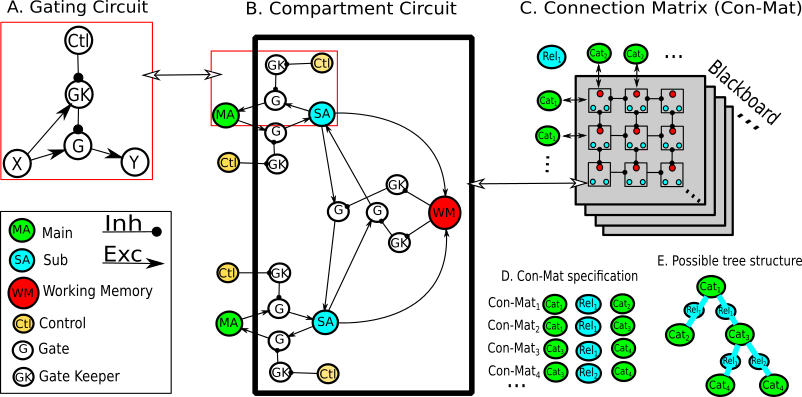
\includegraphics[width=1.00\columnwidth]{figures/part_IV/gating_circuit3}
    \caption{The Neural Blackboard architecture.
      \textbf{A.} Gating circuit that allows the implementation of conditional neural activity transfer between Neural assemblies X and Y through a gate assembly.
      The gate keeper assembly (GK) is activated by the X assembly and then inhibits the gate assembly (G).
      To let information flow through the gate assembly, a control assembly (Ctl) must therefore inhibit the gate keeper assembly.
      \textbf{B.} Architecture of a single compartment circuit of a connection matrix.
      Six gating circuits are arranged in a way that makes conditional bidirectional neural activity flow between two main assemblies possible.
      Control assemblies regulate the direction of information flow and allow the activation of sub assemblies.
      The two sub assemblies excite the working memory assembly which, once activated, encode the binding of the main assemblies and allow activation to flow between them if the controls allow it too.
      \textbf{C.} Each connection matrix contain n by m compartment circuits that encode the same relationship type between the same pair of assembly categories.
      There are $m$ available assemblies for one category and $n$ available assemblies for the complementary category and only one cell circuit can activate its working memory assembly to link two particular assemblies due to mutual row and column inhibition of cells in the connection matrix.
      The size of the connection matrix effectively represents memory limitations.
      A blackboard is composed of an arbitrary number of connection matrices that encode different relationship types for a pair of assembly categories.
      \textbf{D.} A blackboard is composed of multiple connection matrices, where each of them is defined by two node categories and a relationship type between them.
      \textbf{E.} Example of a possible tree structure that can be represented based on the specified connection matrices. }
      \label{Blackboard}
  \end{center}
\end{figure*}


Nodes in Figures {\ref{Blackboard}}.A and {\ref{Blackboard}}.B represent neural assemblies that can be interpreted as linked spiking neural populations.
The most basic component of the NBA is a ``Gating Circuit'' illustrated in Figure {\ref{Blackboard}}.A.
The main idea is that neural activity would flow from the assembly X to the assembly Y, but is blockedby the Gake Keeper (GK) assembly, 
which itself is excited by assembly X.
So to allow directional activity flow from X to Y, a Control (Ctl) assembly has to inhibit the GK assembly.
Notice that it is trivial to extend the gating circuit for bidirectional control of activity flow as illustrated in Figure {\ref{Blackboard}}.B.
Introducing bidirectional conditional control signals is what gives the NBA the possibility of implementing separately queries like 'what follows X?' or 'what follows Y?'.

The second basic component of the NBA is a proposal for working memory (WM).
Persistent neural activity in response to stimuli is considered to be the neural process underlying active (working) memory, and its implementation is hypothesized to be based on excitatory reverberation\citep{wang2001synaptic}.
Based on this, the NBA considers a Delay Activity\citep{de_Kamps_2005} mechanism as a biologically plausible implementation of WM. It consists on a neural assembly, that after being excited beyond a certain threshold, achieved by the coactivation of input populations, will maintain a constant amount of activation for a short period of time. By maintaining its activity, WM acts as a short lived bidirectional link between two assemblies. This mechanism can be considered as the creation of an implicit pointer from one assembly to the other, such that future reactivation of one assembly can be driven from the other to perform query operations. This conforms a ``Memory Circuit'' as depicted in Figure {\ref{Blackboard}}.B.

Two bidirectional ``Gating Circuits'' connected by a ``Memory Circuit'' form a ``Compartment Circuit'' capable of implementing variable binding and query operations.
The key point of this circuit is that Main assemblies (MA), representing grounded concepts or instances of variables types, activate Sub assemblies (SA) 
if a control signal driven by another mechanism allows it.
Then coactivation of SAs is what realizes a temporary binding of MAs by activating WM.
So one ``Compartment Circuit'' models specifically the neural activity of a variable binding operation.
It is operated by a mechanism that drives control signals simultaneously in multiple ``Compartment Circuits'' to instantiate binary tree like data structures on which query/unbinding operations can be performed later. 

As might be evident by now, applying the NBA to syntactic processing in language consists of two simple assumptions.
First, equating the parsing mechanism to the control mechanism that coordinate binding events of words and word types and phrase types.
Second, determining the number of compartment circuits necessary to instantiate a complete syntactic structure and the content of MA nodes from a grammar theory.
In this work we will only employ a phrase grammar and bottom-up parsing scheme following theoretical assumptions of selected neuroimaging experiments.
Nonetheless, a promising feature of the NBA is that it has the flexibility to test any arbitrary parsing mechanism incorporating top-down considerations and an important variety of alternative theories of grammar based on binary trees.
For example dependency grammars that assume multiple direct word bindings instead of the hierarchical phrase bindings modelled in this work have been employed in previous simulations\citep{van_der_Velde_2010}.

To understand how a sentence is processed in the NBA, let us consider first the simplest case of binding two words, like ``Sad student'', 
belonging to grammatical categories instantiated in the MAs of one ``Compartment Circuit'', such that one MA is an ``Adjective'' corresponding to ``sad'' and the other one 
is a ``Noun'' corresponding to ``student''.
The MAs activate with timings corresponding to word presentation, so we are assuming that words were recognized to motivate their corresponding instantiated grammatical 
categories before we attempt to link them.
Then an assumed parsing mechanism determines that a link operating on ``Adjective'' and ``Noun'' types is necessary in the blackboard, driving activity in several 
``Compartment Circuits'' from which only one, that we consider as the recruited ``Comparment Circuit'', completes coactivation of SAs to drive WM and realize binding between the word types.

In the case of a complete phrase, like ``Fat sad student'', if we are assuming the instantiation of phrase types that form a hierarchical tree theorized by a phrase grammar, 
then the time at which the binding of the instantiated grammatical categories of ``sad student'' takes place would be the time at which a ``Noun Phrase'' is activated and bound 
to the ``Adjective'' corresponding to ``Ten''.

Finally, a ``Connection Matrix'', portrayed in Figure {\ref{Blackboard}}.C, allows the implementation of a complete ``Blackboard''.
It contains variable type relations learned by the ``Blackboard'' as sets of mutually inhibitory ``Compartment Circuits'' that enable the selection of the 
``Compartment Circuits'' requested by the control mechanism.
We portray the ``Blackboard'' as a regular grid for illustrative purposes, although there is already a proof of concept implementation with 
randomly connected networks\citep{van_der_Velde_2011}.
Also implementing a general syntactic control mechanism should be feasible. As suggested by the Feed-forward artificial 
neural networks employed in previous NBA simulations~\citep{van_der_Velde_2010} and recent state of the art feedforward network architectures that have shown top performance for diverse language parsing tasks~\citep{andor2016globally}.
Moreover a more recent proposed extension of the NBA, that imitates the motor circuit of the marine mollusk Tritonia diomedea, 
shows how to generate patterns for sequential activation control\citep{van_Dijk_2015}.
Simulating these higher level mechanisms is a task out of the scope of this work, since we focus specifically on reproducing the neural signatures of variable binding operations.

%\FloatBarrier
% Neural Modelling of variable binding. Tensor framework vs NBA. ANN vs SNN.
%\begin{fullwidth}
\chapter{\label{ch:super_syllables}
Experimental results}
\end{fullwidth}

\begin{chabstract}

In this chapter we report subjects behavioral performance ...

\end{chabstract}


\section{Behavioral performance}
%
The subjects had a behavioral performance above 97\% in both visual and auditory \emph{Pseudoword matching tasks}, except for \emph{Subject 05} that reported concentration span issues over all the acquisition.
Note that due to the experimental design structure, in which we only query few random samples, small score decrements can imply distraction over an important task segment.
\emph{Subjects 01 and 04} reported in the second auditory session that the volume was not high enough to be comfortable, although this did not reflect on their behavioral performance.
So we consider all subjects data apt to neuroimaging interpretation, with caution over \emph{Subject 05}. Behavioral performance details are provided in Table \ref{table:behavior}.


\begin{table}
\begin{tabular}{|>{\bfseries}l|rrr|}
\toprule
Subject &  Visual (\%) &  Auditory (\%) &  Overall (\%) \\
\midrule
01 &        97.22 &          97.22 &    97.22 \\
02 &       100.00 &          98.61 &    99.31 \\
03 &        97.92 &          97.22 &    97.57 \\
04 &        99.31 &          99.31 &    99.31 \\
05 &        92.36 &          88.89 &    90.62 \\
\bottomrule
\end{tabular}
\caption{\textbf{Behavioral performance on the \emph{Pseudowords matching task}:} Performance correspond to correctly identifying if the pseudowords were the same or different, with no answer considered as incorrect. Visual and Auditory headers refer to the sensory modality of the task, where overall is the mean performance of both modalities.}
\label{table:behavior}
\end{table}


\section{Sanity checks}\label{sec:sanity_checks}

\begin{figure*}[ht]
\scriptsize
\hspace{-4ex}
\begin{tabular}{ccc}
\textbf{\Large Subject 1} & \textbf{\Large Subject 2} & \textbf{\Large Subject 3}\\
{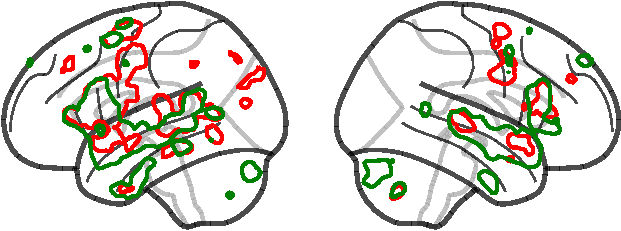
\includegraphics[width=.33\linewidth]{figures/part_II/langloc_01.pdf}}
\hspace{-1ex}
&{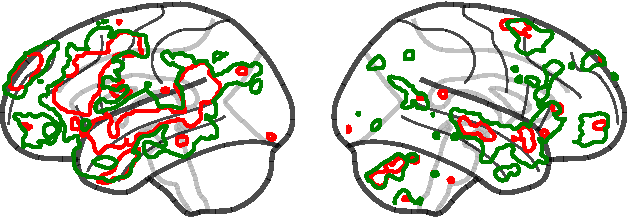
\includegraphics[width=.33\linewidth]{figures/part_II/langloc_03.pdf}}
\hspace{-1ex}
&{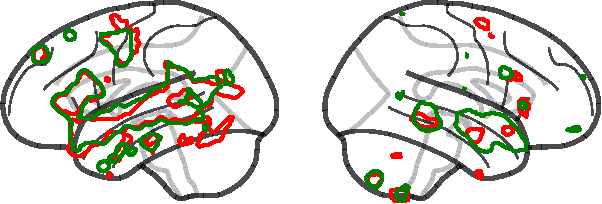
\includegraphics[width=.33\linewidth]{figures/part_II/langloc_04.pdf}}
\hspace{-1ex}\\
\rule{0pt}{6ex}
\textbf{\Large Subject 4} & \textbf{\Large Subject 5} & {}\\
{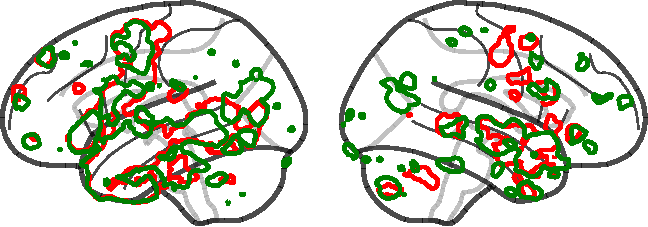
\includegraphics[width=.33\linewidth]{figures/part_II/langloc_05.pdf}}
\hspace{-1ex}
&{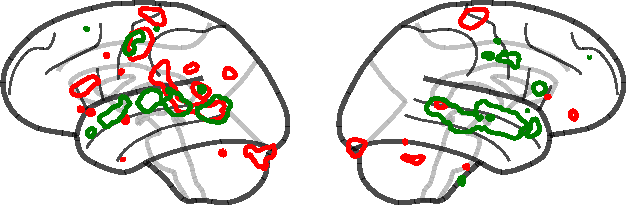
\includegraphics[width=.33\linewidth]{figures/part_II/langloc_06.pdf}}
\hspace{-1ex}
&{
\includegraphics[width=.2\linewidth]{figures/part_II/langloc_legend.pdf}}
\hspace{-1ex} \\
\end{tabular}
\vspace{0ex}
\caption{\textbf{Language localizers:} We show left and right hemispheric contours of the language localizer contrast of word sequences over control stimuli (consonant strings or scrambled recordings), thresholded at a p-value < 10e-3.
Statistical images are projected in the anatomical space of each subject.}
\label{fig:language_localizers}
\end{figure*}

\paragraph{Language localizer activations:}
The contours of the language localizers' contrasts, thresholded at p-value < 10e-3, for both auditory and visual modalities are presented in Figure \ref{fig:language_localizers} for all subjects.
We also show in Figure \ref{fig:language_localizers_radial} the coverage of Mahowald et al. parcels\citep{mahowald2016reliable} by the thresholded language localizers for all subjects.
We see observe an expected left lateralization of the detected language network with more than 40\% coverage of all the language parcels, which covers the fronto-temporal language system that has been well depicted in previous imaging studies\citep{mahowald2016reliable, fedorenko2010new, dehaene2010learning, binder1997human}.
There is variability between the modalities, that particularly disfavors activations of the visual one, in which the subjects can get distracted from perceiving and processing the stimuli more easily, than in the auditory case.
This could be expected from the intrinsic variability of different experimental designs in language localizers as demonstrated by Mahowald et al.\citep{mahowald2016reliable}.
\emph{Subjects 1 and 5} have a defficient coverage that will diminish our capacity to interpret syllabic representation effects along their cortex.
In particular \emph{Subject 5}, who reported concentration problems, have an extremely defficient coverage of the language network.

\begin{figure}[ht]
\scriptsize
\hspace{-4ex}
\begin{tabular}{ccc}
{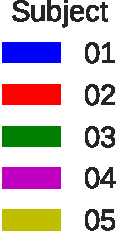
\includegraphics[width=0.1\linewidth]{figures/part_II/subjects_legend.pdf}}
\hspace{-1ex}
&{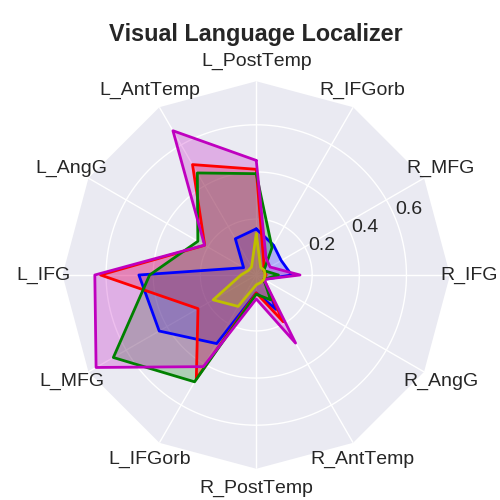
\includegraphics[width=0.45\linewidth]{figures/part_II/visual_langloc_radial.png}}
\hspace{-1ex}
&{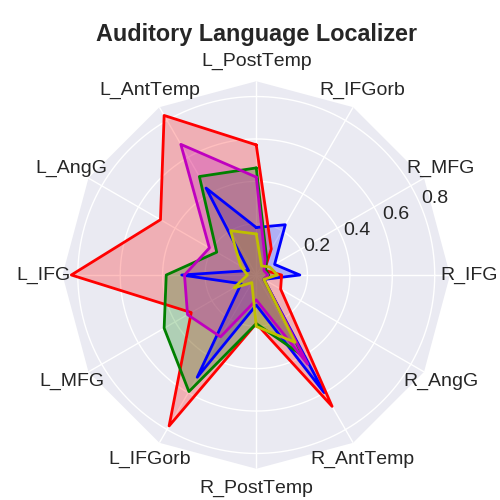
\includegraphics[width=0.45\linewidth]{figures/part_II/auditory_langloc_radial.png}}
\hspace{-1ex}\\
\end{tabular}
\caption{\textbf{Language localizer parcel coverage:}
We show the parcel coverage of each language localizer for the 6 language parcels derived by Mahowald et al. in both hemispheres.
Each subject is represented in a radial chart to emphasize the overall coverage of the language localizers of each subject.
Also the left and right hemisphere parcels have been arranged symmetrically in the radial charts.}
\label{fig:language_localizers_radial}
\end{figure}

\paragraph{Motor activations:}
We verified the integrity of the activation maps of the \emph{Pseudoword matching task} with statistical tests portraying the left and right hand button press contrast.
Z score maps of the left over right button press contrast, for all subjects, are shown in Figure \ref{fig:button_press}, confirming a good statistical separation of hand responses.

\begin{figure}[ht]
\scriptsize
\hspace{-4ex}
\begin{tabular}{cccccl}
\textbf{\Large Subject 1} & \textbf{\Large Subject 2} & \textbf{\Large Subject 3} & \textbf{\Large Subject 4} & \textbf{\Large Subject 5} & {}\\
{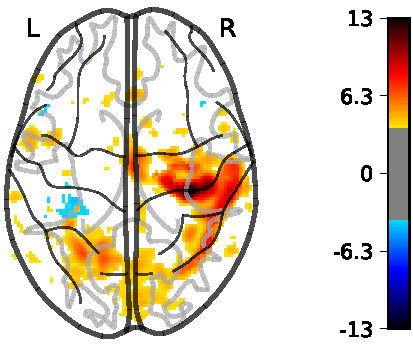
\includegraphics[width=.14\linewidth]{figures/part_II/press_vis_01.pdf}}
\hspace{1ex}
&{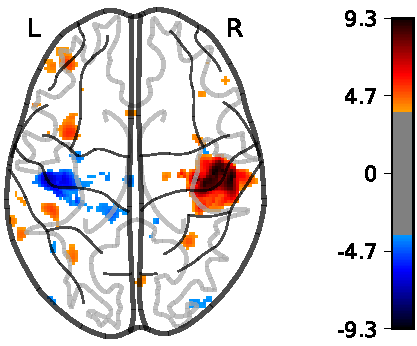
\includegraphics[width=.14\linewidth]{figures/part_II/press_vis_03.pdf}}
\hspace{1ex}
&{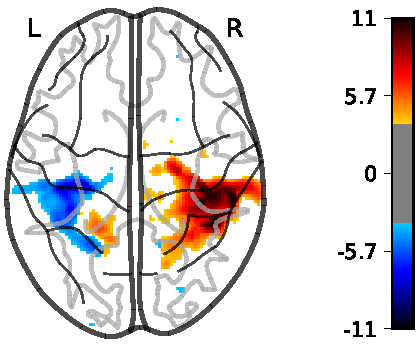
\includegraphics[width=.14\linewidth]{figures/part_II/press_vis_04.pdf}}
\hspace{1ex}
&{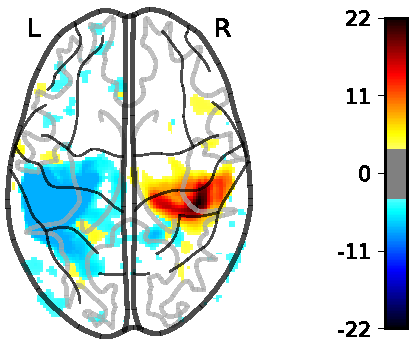
\includegraphics[width=.14\linewidth]{figures/part_II/press_vis_05.pdf}}
\hspace{1ex}
&{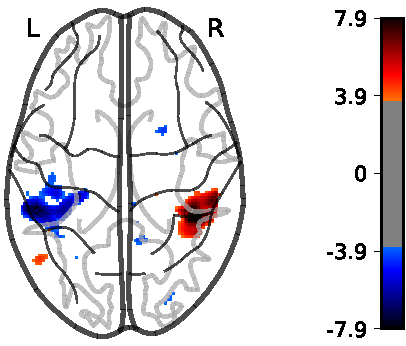
\includegraphics[width=.14\linewidth]{figures/part_II/press_vis_06.pdf}}
\hspace{1ex}
& {} \\
{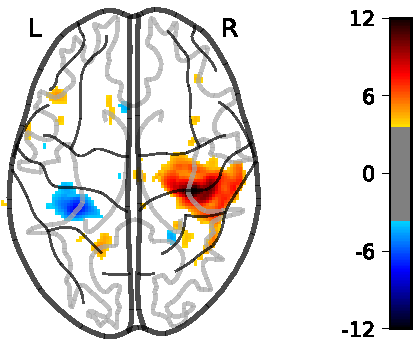
\includegraphics[width=.14\linewidth]{figures/part_II/press_aud_01.pdf}}
\hspace{1ex}
&{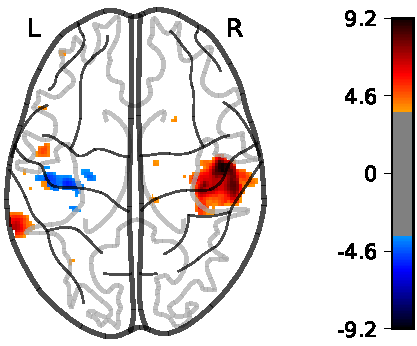
\includegraphics[width=.14\linewidth]{figures/part_II/press_aud_03.pdf}}
\hspace{1ex}
&{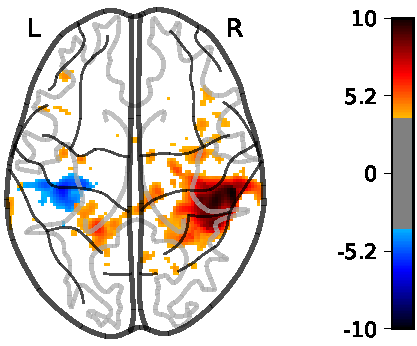
\includegraphics[width=.14\linewidth]{figures/part_II/press_aud_04.pdf}}
\hspace{1ex}
&{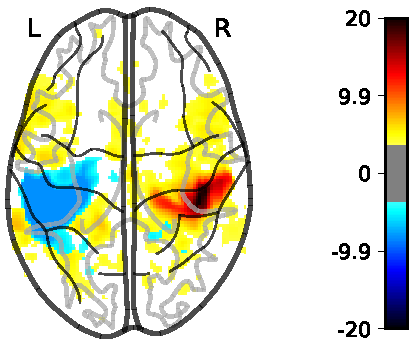
\includegraphics[width=.14\linewidth]{figures/part_II/press_aud_05.pdf}}
\hspace{1ex}
&{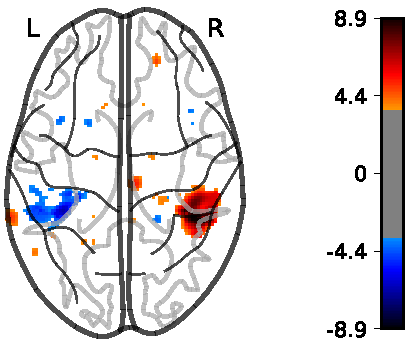
\includegraphics[width=.14\linewidth]{figures/part_II/press_aud_06.pdf}}
\hspace{1ex}
&{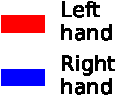
\includegraphics[width=.10\linewidth]{figures/part_II/press_legend.pdf}} \\
\end{tabular}
%\vspace{3ex}
\caption{\textbf{Button press effects:} We show the left button press over right button press contrast Z scores from the auditory modality, thresholded at p < 10e-4, for all subjects. Statistical images correspond to the anatomical space of each subject.}
\label{fig:button_press}
\end{figure}

We also verified that we can employ a Support Vector Classifier (SVC) to distinguish individual left and right button press activation maps derived from the \emph{Pseudoword matching task} General Linear Model (GLM).
As can be seen in Table \ref{table:clic}, we achieve high classification scores of right and left button press events for all subjects.
Moreover as would be expected, the classification generalize across sensory modalities.

\begin{table}
\begin{tabular}{|>{\bfseries}l|rrrrr|}
\toprule
(Train, Test) & (V, V) & (A, A) & (V, A) & (A, V) & (V-A, V-A) \\
Subject & (\%) &  (\%)   & (\%)  & (\%)  &   (\%)\\
\midrule
01      &   84.38*** &   93.50*** &   80.84*** &   76.94*** &           90.88*** \\
02      &   95.38*** &   92.50*** &   84.03*** &   93.03*** &           95.31*** \\
03      &   98.00*** &   99.00*** &   93.91*** &   98.75*** &          100.00*** \\
04      &   97.38*** &   99.50*** &   97.50*** &   98.72*** &          100.00*** \\
05      &   86.62*** &   77.62*** &   90.12*** &   74.28*** &           93.56*** \\
\bottomrule
\end{tabular}
\vspace{5ex}
\caption{\textbf{Classification of left and right button press maps of \emph{Pseudoword matching task}:} \emph{"V"} corresponds to the Visual modality and \emph{"A"} to the Auditory modality. \emph{"V-A"} corresponds to pooling together both datasets for training and testing.}
\label{table:clic}
\end{table}

\blankfootnote{\emph{chance: 50\% \\ * : p < 10e-2,\\ ** : p < 10e-3,\\ *** : p < 10e-4 \\ Bonferroni corrected for 25 similar tests performed}}

\paragraph{Visual activations:}
We verified the statistical effects of left and right syllable position in the Visual hOc1 region.
In the experimental design we asked the subjects to fixate a centered green dot before stimuli presentation.
So we expected, from well known retinotopic effects in the primary visual cortex \citep{tootell1998retinotopy}, to see an hemispheric partition of left and right syllable position effects, such that left syllable effects would be emphasized in the right hemisphere and right syllable effects in the left hemisphere.
This was the case, as can be seen in Figure \ref{fig:retinotopy}, where \emph{Subjects 1 and 4} have the clearest retinotopic activations.
Nonetheless we can also appreciate in the images that some subjects did not manage to completely follow the fixation instruction, since effects of both positions are present together in both hemispheres.


\begin{figure*}[ht]
\scriptsize
\vspace{2ex}
\hspace{-4ex}
\begin{tabular}{cccccl}
\textbf{\Large Subject 1} & \textbf{\Large Subject 2} & \textbf{\Large Subject 3} & \textbf{\Large Subject 4} & \textbf{\Large Subject 5} & {}\\
{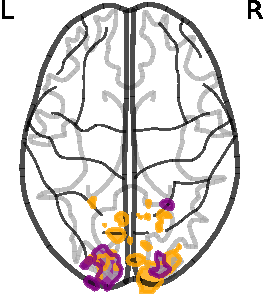
\includegraphics[width=.13\linewidth]{figures/part_II/retinotopy_01.pdf}}
\hspace{1ex}
&{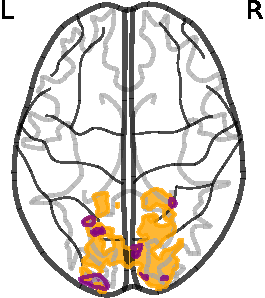
\includegraphics[width=.13\linewidth]{figures/part_II/retinotopy_03.pdf}}
\hspace{1ex}
&{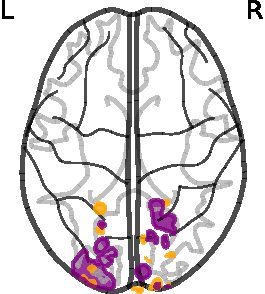
\includegraphics[width=.13\linewidth]{figures/part_II/retinotopy_04.pdf}}
\hspace{1ex}
&{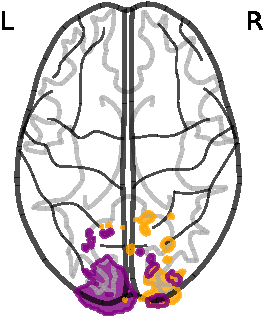
\includegraphics[width=.13\linewidth]{figures/part_II/retinotopy_05.pdf}}
\hspace{1ex}
&{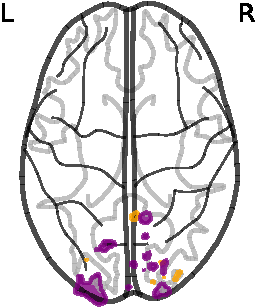
\includegraphics[width=.13\linewidth]{figures/part_II/retinotopy_06.pdf}}
\hspace{-1ex}
&{
\includegraphics[width=.12\linewidth]{figures/part_II/retinotopy_legend.pdf}}
\hspace{-1ex} \\
\end{tabular}
\vspace{3ex}
\caption{\textbf{Retinotopic effect:} We show first and second syllable position effects masked by the Visual hOc1 region, thresholded at a p-value < 0.005.
Statistical images correspond to the anatomical space of each subject.}
\label{fig:retinotopy}
\end{figure*}



\section{Visual representations}

Due to retinotopy and the large size of the text presented in the \emph{Pseudowords matching task}, we expected to be able to decode visual representations and demonstrate superposed representations trivially implied by retinotopy.

As can be seen in Table \ref{table:visual_word_pred}


\begin{figure}[ht]
\scriptsize
\vspace{2ex}
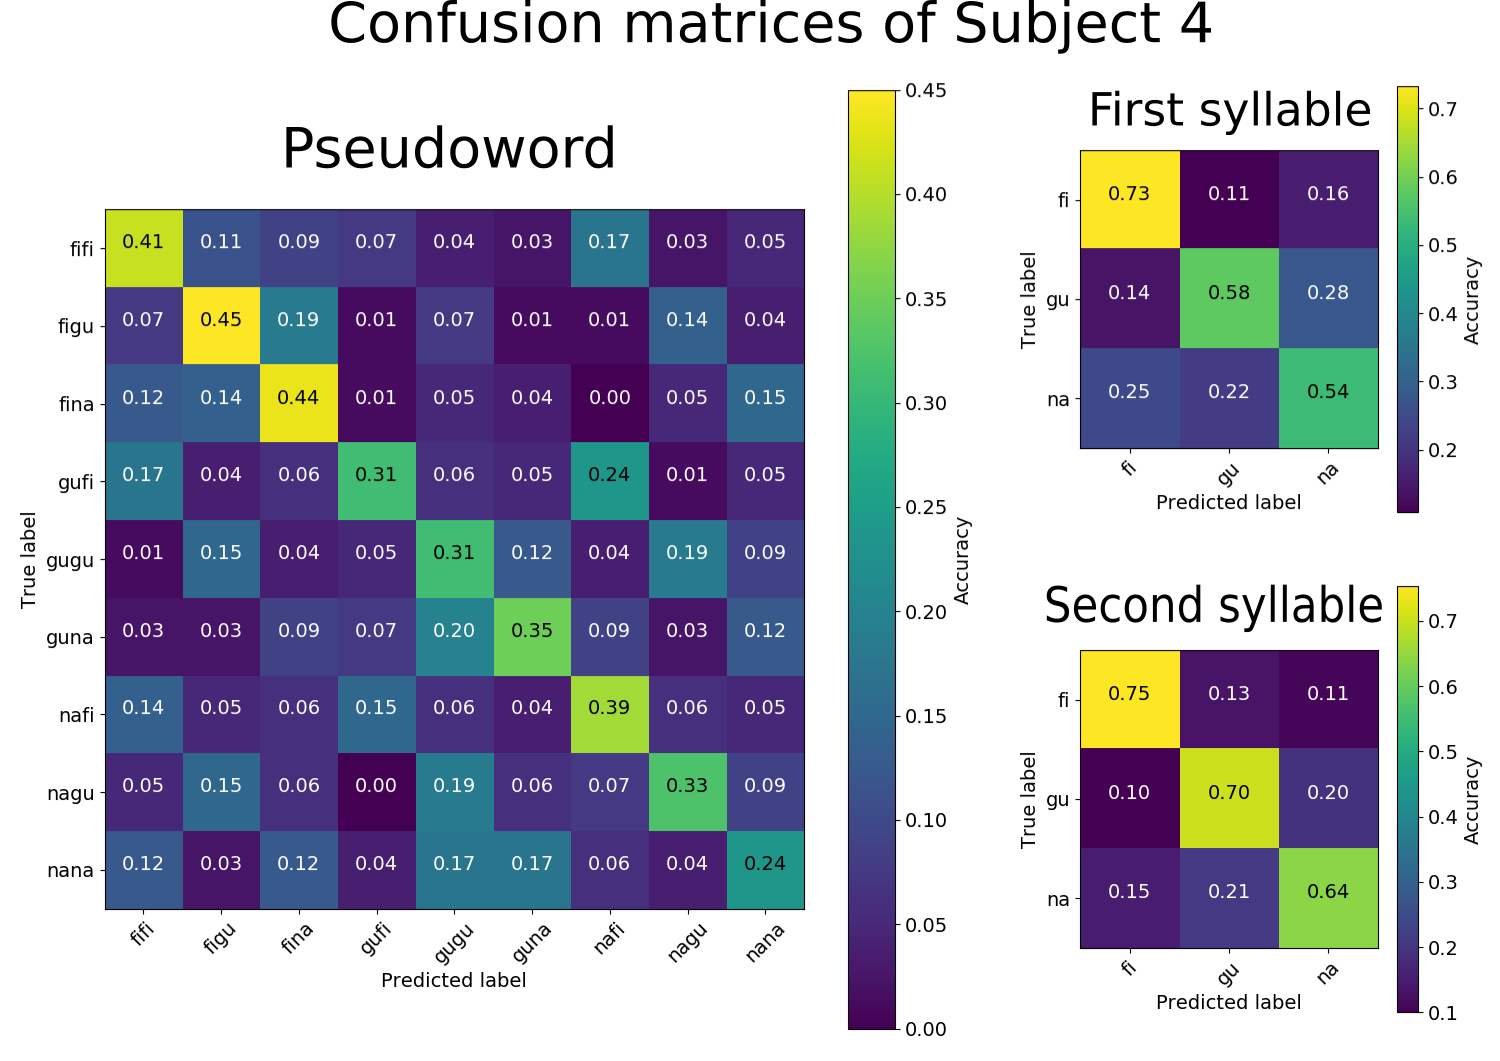
\includegraphics[width=1.\linewidth]{figures/part_II/confusion_subject_4.png}
\vspace{3ex}
\caption{\textbf{Confusion matrices of \emph{Subject 4}:}
We show }
\label{fig:visual_confusion}
\end{figure}


\begin{table*}
\begin{tabular}{lllllllllll}
\toprule
Condition &    fifi &    figu &    fina &    gufi &    gugu &    guna &    nafi &    nagu &    nana &    Mean \\
Subject &         &         &         &         &         &         &         &         &         &         \\
\midrule
01      &  0.30** &  0.23** &  0.29** &   0.19* &   0.19* &    0.15 &   0.16* &    0.12 &  0.20** &  0.20** \\
02      &    0.17 &   0.20* &   0.21* &    0.16 &    0.15 &    0.09 &  0.23** &   0.15* &    0.12 &  0.17** \\
03      &   0.25* &    0.19 &   0.21* &    0.14 &  0.17** &    0.12 &  0.19** &   0.14* &    0.11 &  0.17** \\
04      &  0.41** &  0.45** &  0.44** &  0.31** &  0.31** &  0.35** &  0.39** &  0.33** &  0.24** &  0.36** \\
05      &   0.20* &  0.23** &    0.16 &    0.14 &  0.20** &   0.16* &   0.15* &    0.14 &    0.11 &  0.17** \\
\bottomrule
\end{tabular}
\vspace{2ex}
\caption{\textbf{Classification of left and right button press maps of \emph{Pseudoword matching task}:} \emph{"V"} corresponds to the Visual modality and \emph{"A"} to the Auditory modality. \emph{"V-A"} corresponds to pooling together both datasets for training and testing.}
\label{table:visual_word_pred}
\end{table*}

\vspace{30ex}
\blankfootnote{\emph{chance: 50\% \\ * : p < 10e-2,\\ ** : p < 10e-3,\\ *** : p < 10e-4 \\}}


\begin{figure*}[ht]
\scriptsize
\vspace{2ex}
\hspace{-4ex}
\begin{tabular}{ccccc}
\textbf{\Large Subject 1} & \textbf{\Large Subject 2} & \textbf{\Large Subject 3} & \textbf{\Large Subject 4} & \textbf{\Large Subject 5}\\
{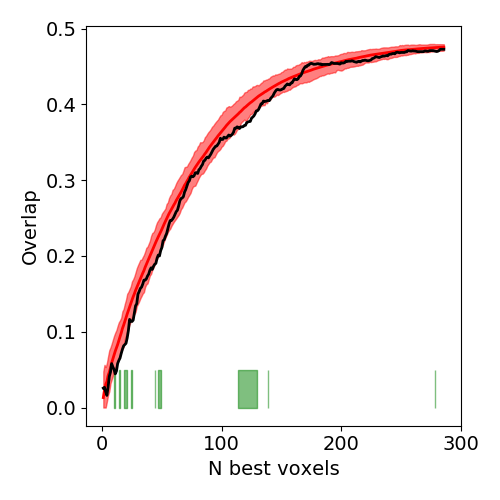
\includegraphics[width=.19\linewidth]{figures/part_II/locality/visual/locality_test_01.png}}
\hspace{0ex}
&{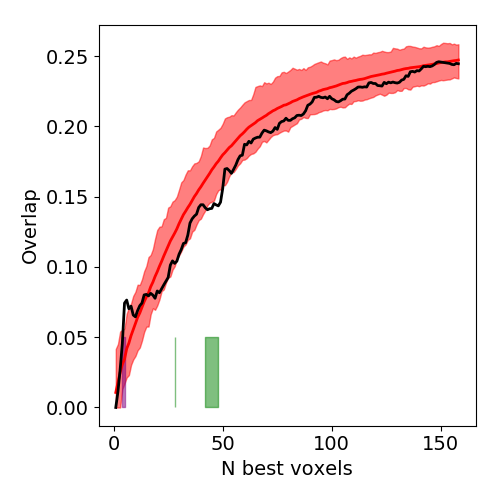
\includegraphics[width=.19\linewidth]{figures/part_II/locality/visual/locality_test_03.png}}
\hspace{0ex}
&{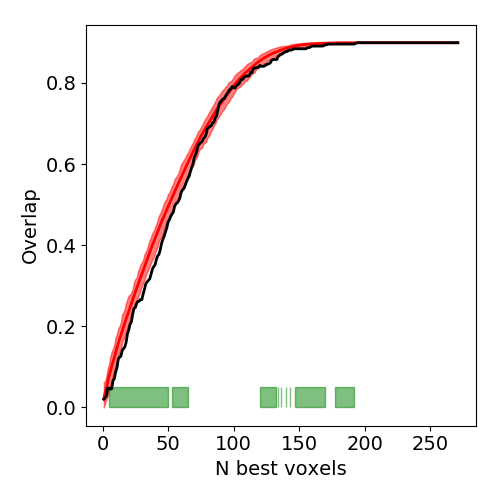
\includegraphics[width=.19\linewidth]{figures/part_II/locality/visual/locality_test_04.png}}
\hspace{0ex}
&{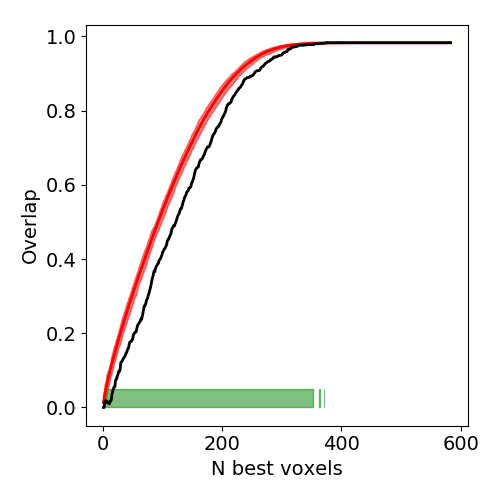
\includegraphics[width=.19\linewidth]{figures/part_II/locality/visual/locality_test_05.png}}
\hspace{0ex}
&{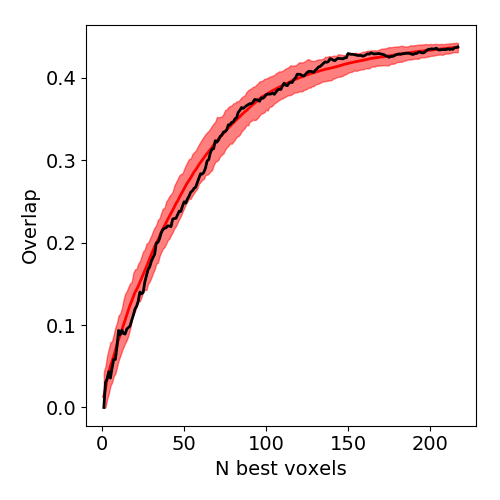
\includegraphics[width=.19\linewidth]{figures/part_II/locality/visual/locality_test_06.png}}
\hspace{-1ex} \\
\end{tabular}
\vspace{3ex}
\caption{\textbf{Partitioned spatial distribution of visual representations:} We show }
\label{fig:visual_locality}
\end{figure*}


\begin{table*}
\begin{tabular}{llllllllll}
\toprule
Test & Relatedness &          &        & No roles &         &        & Superposition &          &         \\
Overlap &        Diff & Position &   None &     Diff & Crossed &   None &          Diff & Position & Crossed \\
Subject &             &          &        &          &         &        &               &          &         \\
\midrule
01      &       0.018 &    0.115 &  0.097 &   -0.046 &   0.052 &  0.097 &       0.063** &    0.115 &   0.052 \\
02      &       0.000 &    0.000 &  0.000 &    0.000 &   0.000 &  0.000 &         0.023 &    0.110 &   0.088 \\
03      &       0.003 &    0.109 &  0.106 &    0.006 &   0.112 &  0.106 &        -0.003 &    0.109 &   0.112 \\
04      &     0.064** &    0.117 &  0.053 &   -0.018 &   0.035 &  0.053 &       0.082** &    0.117 &   0.035 \\
05      &       0.011 &    0.098 &  0.088 &    0.031 &   0.119 &  0.088 &        -0.020 &    0.098 &   0.119 \\
\bottomrule
\end{tabular}
\vspace{10ex}
\caption{\textbf{Classification of left and right button press maps of \emph{Pseudoword matching task}:} \emph{"V"} corresponds to the Visual modality and \emph{"A"} to the Auditory modality. \emph{"V-A"} corresponds to pooling together both datasets for training and testing.}
\label{table:superposition tests}
\end{table*}

\vspace{40ex}
\blankfootnote{\emph{chance: 50\% \\ * : p < 10e-2,\\ ** : p < 10e-3,\\ *** : p < 10e-4 \\ Bonferroni corrected for 25 similar tests performed}}



\section{Auditory representations}






% \section{Language representations}


% \paragraph{\emph{Pseudoword matching task} effects:}
% Neural activations related to differences between the nine bi-syllabic conditions are spread across the cortex for all subjects, as reveals the simple check of the contour of an F test, thresholded at p-value < 0.0001, of any difference between conditions, shown in Figure \ref{fig:any-effects}.
% Nonetheless, to pursue the objective of this work, we needed to separate regions encoding the stimuli as a whole (holistic representation) from regions encoding stimuli parts (distributed representation) that might further follow the superposition principle (superposed representation).
% From an statistical point of view, this means that we wanted to discriminate regions on which there are only effects of the first and second syllable position from regions on which there is an interaction effect that would suggest additional encoding terms contradicting the superposition principle.
% In Figure \ref{fig:syllable_effects} we pool together the filled contours of the statistical effects, thresholded at p-value < 0.0001, of any syllable position and their interaction from both auditory and visual modalities.
% From the high level perspective of Figure \ref{fig:syllable_effects}, we can observe that all effects spread around the whole brain and then occupy similar functional regions in all subjects, although position effects seem to occupy a higher portion of the cortex.

% \begin{figure}[ht]
% \scriptsize
% \vspace{5ex}
% \hspace{-4ex}
% \begin{tabular}{ccccc}
% \textbf{\Large Subject 1} & \textbf{\Large Subject 2} & \textbf{\Large Subject 3} & \textbf{\Large Subject 4} & \textbf{\Large Subject 5}\\
% {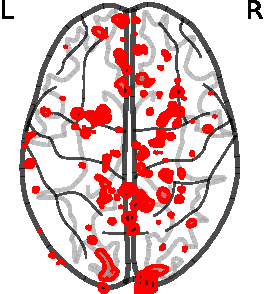
\includegraphics[width=.165\linewidth]{figures/part_II/any-effects_01.pdf}}
% \hspace{1ex}
% &{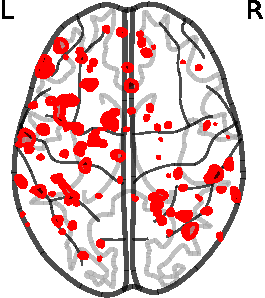
\includegraphics[width=.165\linewidth]{figures/part_II/any-effects_03.pdf}}
% \hspace{1ex}
% &{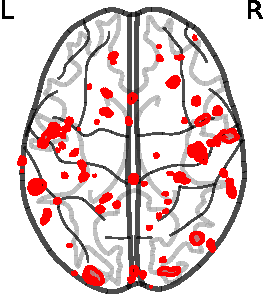
\includegraphics[width=.165\linewidth]{figures/part_II/any-effects_04.pdf}}
% \hspace{1ex}
% &{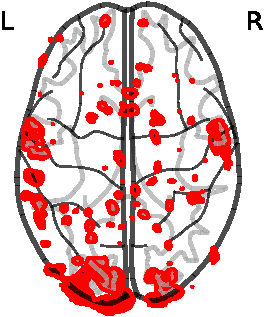
\includegraphics[width=.165\linewidth]{figures/part_II/any-effects_05.pdf}}
% \hspace{1ex}
% &{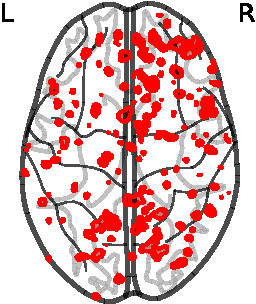
\includegraphics[width=.165\linewidth]{figures/part_II/any-effects_06.pdf}}
% \hspace{1ex}\\
% \end{tabular}
% \vspace{3ex}
% \caption{\textbf{Any stimuli difference:} We show the contour of the statistical F test reflecting any difference between the bi-syllabic conditions, thresholded at a p-value < 0.0001. Statistical images correspond to the anatomical space of each subject.}
% \label{fig:any-effects}
% \end{figure}


% \begin{figure*}[ht]
% \scriptsize
% \hspace{-4ex}
% \begin{tabular}{ccc}
% \textbf{\Large Subject 1} & \textbf{\Large Subject 2} & \textbf{\Large Subject 3}\\
% {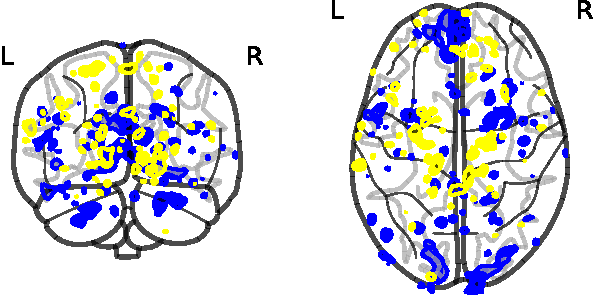
\includegraphics[width=.33\linewidth]{figures/part_II/all-effects_01.pdf}}
% \hspace{-1ex}
% &{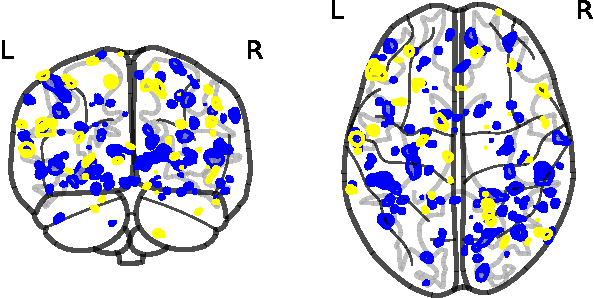
\includegraphics[width=.33\linewidth]{figures/part_II/all-effects_03.pdf}}
% \hspace{-1ex}
% &{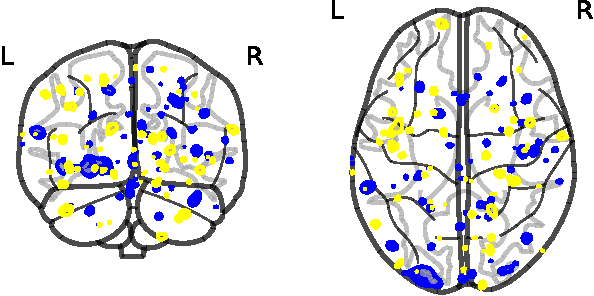
\includegraphics[width=.33\linewidth]{figures/part_II/all-effects_04.pdf}}
% \hspace{-1ex}\\
% \rule{0pt}{6ex}
% \textbf{\Large Subject 4} & \textbf{\Large Subject 5} & {}\\
% {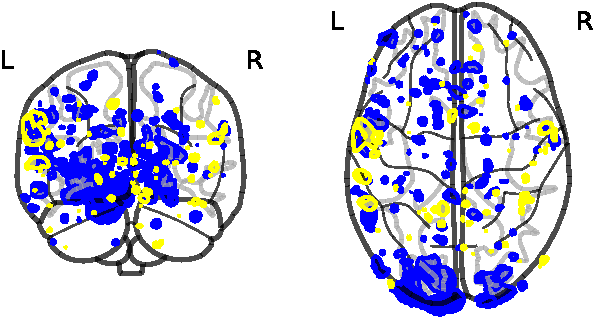
\includegraphics[width=.33\linewidth]{figures/part_II/all-effects_05.pdf}}
% \hspace{-1ex}
% &{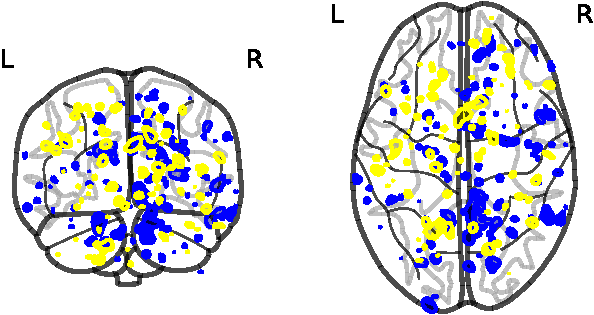
\includegraphics[width=.33\linewidth]{figures/part_II/all-effects_06.pdf}}
% \hspace{-1ex}
% &{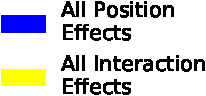
\includegraphics[width=.2\linewidth]{figures/part_II/all-effects_legend.pdf}}
% \hspace{-1ex} \\
% \end{tabular}
% \vspace{3ex}
% \caption{\textbf{Pseudoword matching task effects:} We show blobs corresponding to the statistical test of main effects (effect of first and second position) and interaction (sign of holistic representation) for the \emph{Pseudoword matching task}, thresholded at a p-value < 0.0001.
% We consider blobs from both auditory and visual modalities of the task together, to portray the extent of the possible effects. Statistical images correspond to in the anatomical space of each subject.}
% \label{fig:syllable_effects}
% \end{figure*}


% \paragraph{Searchlight networks derived:}
% Since we designed our stimuli to be interpreted from the point of view of morphological processing (language processing), we employed the statistical effect maps from both modalities to determine a sub-network of the identified language network in each subject that would be used for further classification with the searchlight procedure presented in the methods section \ref{sec:searchlight_classification}.
% We show in in Figure \ref{fig:searchlight_regions} the obtained searchlight networks for each subject, while emphasizing that both holistic and superposed representation candidate regions are captured inside the identified language networks.
% Notice that both candidates are spread on the whole fronto-temporal language system and that \emph{Subjects 2 and 4} have broad searchlight networks corresponding to their broader language network activations, as depicted in Figure \ref{fig:language_localizers}.


% \begin{figure}[ht]
% \scriptsize
% \hspace{-4ex}
% \begin{tabular}{cc}
% \textbf{\Large Subject 1} & \textbf{\Large Subject 2}\\
% {\includegraphics[width=.5\linewidth]{figures/part_II/searchlight-regions_01.pdf}}
% \hspace{-1ex}
% &{\includegraphics[width=.5\linewidth]{figures/part_II/searchlight-regions_03.pdf}}
% \hspace{-1ex}\\
% \rule{0pt}{6ex}
% \textbf{\Large Subject 3} & \textbf{\Large Subject 4}\\
% {\includegraphics[width=.5\linewidth]{figures/part_II/searchlight-regions_04.pdf}}
% \hspace{-1ex}
% &{\includegraphics[width=.5\linewidth]{figures/part_II/searchlight-regions_05.pdf}}
% \hspace{-1ex}\\
% \rule{0pt}{6ex}
% \textbf{\Large Subject 5} & {}\\
% {\includegraphics[width=.5\linewidth]{figures/part_II/searchlight-regions_06.pdf}}
% \hspace{-1ex}
% &{\includegraphics[width=.3\linewidth]{figures/part_II/searchlight-regions_legend.pdf}}
% \hspace{-1ex} \\
% \end{tabular}
% \vspace{3ex}
% \caption{\textbf{Searchlight networks:} We show the derived searchlight network for each subject. We separate for illustrative purposes the portion of the network derived from interaction effects (Holistic candidate) and from exclusive main effects (Superposition candidate). Images correspond to the anatomical space of each subject.}
% \label{fig:searchlight_regions}
% \end{figure}

%\FloatBarrier
% Neuroimaging techniques. fMRI and ECoG techniques.
%\begin{fullwidth}
\chapter{\label{ch:super_methods}
The syllables superposition experiment}
\end{fullwidth}

\begin{chabstract}

In this chapter we present methods

\end{chabstract}

\section{Methods}

{\label{488128}}

\subsection{Simulation framework}\label{simulation-framework}

We assume that the NBA lives in the cortex, and seek a good compromise between realistic modelling of the cortical dynamics and the tractability of the simulation.
State-of-the-art simulations of larger cortical structures are based on point model neurons that allow the inclusion of biological details such as synaptic dynamics and adaptation, but are restricted to about the size of a cortical column \cite{potjans2012cell}.
For larger scale networks, such as ours, a population-based approach is currently the only feasible approach.
The two choices are: rate based models or population density techniques (PDTs).
In rate based models, the population is described by a single variable, usually related to the population firing rate or average membrane potential of neurons in the population. 
A prominent example is the  Wilson-Cowan equation \cite{wilson1972excitatory}, which describes the dynamics of the population activity as a first order linear differential equation driven by inputs.
Another example is the Jansen-Rit model \cite{jansen1995electroencephalogram}, which is primarily motivated by phenomenological considerations.
In both examples, the relationship with the underlying neural state is unclear. We have opted for PDTs, also a population based approach, but one where the relationship with the dynamics of a group of spiking point model neurons can be made rigorous.
Although they are computationally more expensive than rate based models, they are easier to manage than a full-blown model using spiking neurons, which would need hundreds of thousands of neurons at the scale of the cortical network considered here.
We will briefly set out the assumptions that we use in modelling populations and describe the numerical methods involved.

Consider a leaky-integrate-and-fire (LIF) neuron, which is characterized by a single state variable: the membrane potential.
If the neuron has a potential different from its equilibrium potential, or when it experiences an external drive, for example generated by a synaptic current, the potential evolves according to:

\begin{equation}
\tau \frac{dV}{dt} = -(V - V_{rev}) + I(t).
\label{eq-lif}
\end{equation}

Here $V$ is the membrane potential in V, $\tau$ the membrane time constant in s, $V_{rev}$ the reversal potential and $I(t)$ and external current, which may comprise contributions from other neurons in the form of spikes, and therefore may be stochastic.
If the membrane is driven far above the equilibrium potential, at a potential $V_{th}$, the threshold, the neuron spikes.
We assume it will be inactive for an absolute refractive period $\tau_{ref}$ and then finds itself reset to the equilibrium potential after that.  
This scenario is easy to simulate: using a simulator like NEST \cite{gewaltig2007nest}, or BRIAN \cite{stimberg2014equation}, one can create populations of LIF neurons.
In the simplest case a population is driven by synthetically generated input spike trains, where the spike train events are created by a random generators.
The default assumption is that inter-spike intervals are Poisson distributed, although this can be extended to non-Markov processes \cite{lai2017population}.
It is clear that $I(t)$ in Eq. \ref{eq-lif} now should be considered as a stochastic variable and that the threshold crossings of LIF neurons themselves are stochastic events as a consequence.
Fig. \ref{fig:pdt-case} A  demonstrates a simple scenario: a population of 10000 LIF neurons, driven by a stochastic input - Poisson generated spike trains, where each LIF neuron experiences about 800 input spikes per second.
The simulation shows a spike raster of the population response:
first nothing: although each LIF neuron receives input spikes and as a consequence has its membrane potential driven up, none of the neurons have reached threshold;
then a spike volley: most neurons hit threshold at approximately the same time;
followed by a period of relative silence: only interrupted by a few stragglers;
at last a gradually achieved final neural state of asynchronous random firing.
More complex networks can be formed by feeding the output spikes of one population into other populations.

This is a fascinating but unwieldy process and statistical methods have been used to describe it at the population level \cite{stein1967some,knight1972dynamics,omurtag2000simulation}.
A population is described by a density function, which expresses how the population is distributed over state space.
For LIF neurons this is a function $\rho(V)$, where $\rho(V)dV$ is the fraction of neurons with their membrane potential in interval $[V, V + dV)$ (when we integrate the density function over a certain state interval, we will refer to the  result as  the amount of \emph{mass} in that interval).
The initial distribution of the neurons in the population must be chosen, but the evolution of the density is tractable.
It is clear that neurons move through state space due to the deterministic neural dynamics, Eq \ref{eq-lif} for LIF neurons, and also go transitions due to the input spikes.
The collective contribution of the stochastic process to the evolution of the density profile can be  modelled using a Poisson master equation \cite{crispin1994handbook}; the contribution of the deterministic dynamics  can be modelled using an advection equation (see \cite{omurtag2000simulation} for a lucid explanation). 


As a consequence, the process of simulating thousands of neurons is now replaced by modelling the evolution of a density which is given by a single equation:

\begin{equation}
\frac{\partial \rho}{\partial t} -\frac{1}{\tau}\frac{\partial}{\partial v}(\rho v) = \int dh p(h) \nu (\rho(v - h) -\rho(v)),
\label{eq-synapse}
\end{equation} 

Here $p(h)$ is the distribution of synaptic efficacies, $\nu$ the frequency of the incoming spike trains, $\rho$ the density function, $t$ the time since start of simulation and $v$ the membrane potential.
Mass that is being pushed across threshold corresponds to neurons spiking; consequently  the firing rate of the population can be calculated directly from the mass flux across threshold.

Efficient and stable simulation methods are available \cite{nykamp2000population, de2003simple, de2013generic, iyer2013influence}, and remarkably, the process of solving Eq. \ref{eq-synapse} is computationally less expensive for LIF neurons than the direct simulation using NEST \cite{nykamp2000population}.
The process of keeping track of a single density function, and the communication between populations using firing rates rather than individual spikes, frees the modeller from keeping track of thousands of spikes per second and leads to simpler simulations.
Figure \ref{fig:pdt-case} shows the very close correspondence between direct simulations of LIF spiking neurons and population density results.
It shows, first, that the simulation results indeed are very close to that of the spiking simulation, and second, that Wilson-Cowan dynamics must be tuned in a way that PDTs do not: the correct steady state activation must be provided to the Wilson-Cowan dynamics in the form of a sigmoid, while in PDTs the correct steady state firing rate is calculated from first principles - input firing rate, synaptic efficacies and neural parameters - without any need for tuning. 


\begin{figure}[h!]
  \begin{center}
    \includegraphics[width=1.0\columnwidth]{figures/pdt_overview.pdf}

    \caption{\textbf{A.} A spike raster showing an LIF population undergoing a jump response.
        Neurons are at equilbrium at $t = 0$. From $t=0$ each neuron receives a Poisson distributed input spike train ($\lambda$ = 800 Hz, $h= 0.03$, i.e. an input spike raises the PSP by 3\% of the difference between threshold and equilibrium potential, $\tau = 50$ ms, following \cite{omurtag2000simulation}).
        \textbf{B.} Firing rate calculated from the PDT method (solid curve), compared to firing rate from spiking neuron simulation (red markers).
        \textbf{C.} The density calculated by the PDT method (solid curve) at $t=0.3$ s, compared to a histogram of the membrane potential over the population at the
        same time.
        \textbf{D.} Wilson-Cowan prediction for the firing rate, compared to PDT result. Importantly, Wilson-Cowan output must be tuned: the steady state value to which it converges is not predicted by the Wilson-Cowan equations, but must be provided as a sigmoid. 
       In contrast, the PDT method calculates the firing rate from first priciples, and agrees well with the spiking neuron simulation, within statistics.
      }
\label{fig:pdt-case}
  \end{center}
\end{figure}


The population density formalism can be extended to higher dimensional models.
For example, the adaptive-exponential-integrate-and-fire neuron (AdEx) \cite{brette2005adaptive} is a two dimensional model that has the membrane potential and an adaptivity parameter as a variable.
Consequently, the state space is two dimensional.
The motivation behind this model is that first, it includes adaptation, and second that it is the effective approximation of the complex conductance-based processes that take place in a real neuron.
The equations of the model are:

We consider the AdEx model as presented by Brette and Gerstner \cite{brette2005adaptive}, which describes individual neurons by the following equations:
\begin{align}
  C_m \frac{dV}{dt}    & =  -g_l(V - E_l)  + g_l e^{ \frac{(V - V_T)}{\Delta_{T}}} \\
  \tau_w \frac{dw}{dt} & =  a(V-E_l) -w \nonumber
\end{align}

Where $C_m$ is the membrane capacitance, $g_l$ the leak conductance, $E_l$ the leak potential (equivalent to the reversal potential for the LIF), $V_T$ a threshold potential, $\Delta_T$ a shape parameter for the spike, $\tau_w$ the adaptation time constant, $a$ the subthreshold adaptation parameter,  $V$ the membrane potential and $w$ the adaptation parameter. Upon a spike, the neuron is undergoes a transition in $w$: $w \rightarrow w +b$, where $b$ is the spike adaptation parameter.
We use the parameters given by Brette and Gerstner (2005).


\begin{figure}[h!]
  \begin{center}
    \includegraphics[width=1.0\columnwidth]{figures/aexp_overview.pdf}
    \caption{{AdEx dynamics {\label{fig-adex}} Left: Overview of AdEx dynamics.
        Right: a heat plot of the density profile during simulation. On the horizontal axis the membrane potential, on the vertical axis the adaptivity parameter. Note that
 the right figure constitutes a considerable reduction of state space compared to left. For the connectivity parameters we use, the state space on the right is the
part of state space reachable by dynamics.
      }}
  \end{center}
\end{figure}

We illustrate the dynamics of the neuron in Fig. \ref{fig-adex}.
The direction of the dynamics is shown by arrows, the speed of the dynamics by the size of the cells:
big cells implies fast dynamics as the cells represent equidistant time steps.
This shows that at $w =0$ dynamics are leaky,  i.e. towards the equilibrium, except at high values of $V$, on the right, which corresponds to spike generation.
At high values of $w$, there are two effects: stronger leak (larger cells) and a lower (more negative) equilibrium potential, which makes it harder for a cell at high $w$ to be driven across threshold, precisely the effect one expects due to adaptation.
At low $w$, the opposite happens: cells become more excitable.
For very low $w$ values, which can not be reached under cortical conditions, at least not for the parameters we used, there is the theoretical probability of a rebound (neuron always spikes).

A density function now lives in this two dimensional space: $\rho(V,w)$.
The evolution equation is a direct generalization of Eq. \ref{eq-synapse}.
For a model with $n$ state variables $\vec{V}$, a point model takes the form:
\begin{equation}
\tau \frac{d \vec{V}}{dt} = \vec{F}(\vec{V})
\end{equation}
and the density equation:
\begin{equation}
\frac{\partial \rho}{\partial t} + \frac{\partial}{\partial \vec{V}} \cdot \frac{( \vec{F} \rho)}{\tau} = \int dh p(h) \nu (\rho(\vec{V} - \vec{h}) -\rho(\vec{V}))
\end{equation},
where $\vec{h}$ represents the effect of an input spike.

We represent the density function by a heat plot on state space: the highest values or white, low values are red.
We are able to simulate the density function by a method analogous to that of \cite{de2013generica,iyer2013influence}, generalized to two dimensions.
In Fig. \ref{fig-adex} we show the result of a simulation: the density function as a fixed point in time.
As before, we can calculate the firing rate of the population by calculating the the flux across threshold (which is still given by $V= V_{threshold}$, i.e. the right hand side of the grid).

The simulation software, MIIND, is publicly available \url{http://miind.sf.net}. The LIF version of the algorithm has been available for some time \cite{de_Kamps_2008}, while 
the two dimensional version has become available recently \cite{dekamps2017b}.


\subsection{NBA simulation}\label{architectural-decisions}

Previous simulations of the NBA approximate the mean activity of neural assemblies with Wilson Cowan dynamics \cite{Frank_2014}.
Nonetheless, as explained in section \ref{simulation-framework}, direct simulations of leaky-integrate-and-fire (LIF) neurons \cite{omurtag2000simulation} have different transient behaviour than the dynamics described by the Wilson Cowan equations.Since we are interested in modelling the transient dynamics of variable binding in order to compare 
the simulation with real temporally detailed patterns of intracortical neural measurements like ECoG, we feel the need to model spiking neuron dynamics is important.

The decision to use AdEx, rather than LIF neurons has two motivations: first, adaptation is ubiquitous and its inclusion has a substantial impact on the dynamical range
allowed within the constraints of the blackboard architecture. Second,  it has been shown that 2D models, like AdEx, can already predict correctly 96\% of the spikes of 
detailed conductance models\cite{brette2005adaptive}.  Also, this model reproduces many known electrophysiological features, as can be appreciated in the spike-frequency adaptation review of Benda et al. \cite{Benda_2003,Benda_2014}. Our approach is consistent with a trend towards simpler, geometrically motivated  2D   models  that preserve the essence of more complex biophysically motivated models \cite{izhikevich2007dynamical}.

AdEx is now available in  MIIND. To our knowledge this is the first time that the AdEx model will be employed to approximate the neural dynamics of a circuit of this magnitude reproducing cognitive function.

In the case of Delay Activity (DA) populations like Working Memory (WM), we decided as a first approach to model such a mechanism phenomenologically.
We plan to address the different alternatives to model persistent cortical activity with interacting neural populations in future work.
As suggested by de Kamps\cite{de_Kamps_2005} not only models of recurrent excitation but also recurrent inhibition can account for this phenomena.
In the current simulation, a constant firing rate for DAs is kicked off by a specified level of input, resulting in activation  that is sustained for a predetermined period of time.
Contrary to previous simulations \cite{velde2015ambiguity}, we do not consider Sub-Assemblies (SAs) as DA populations.
We find that SAs can show rich and interesting dynamics just by fulfilling their function of mediating activation for WM.

We model Main-Assemblies (MAs)  as receiving input from DA populations, representing word types in some cases, and WM populations representing phrase types in other cases.
We do this to satisfy the assumptions of a phrase grammar that requires representation of deep tree hierarchical structures, so that we can separate the notion of a phrase resulting from previous word type bindings stored in WM, from the recruitment of MAs representing word grammatical category instantiations that take place during sentence processing.
Note that for other grammar types, like dependency grammars considered in previous NBA simulations\cite{velde2015ambiguity}, to consider words as nodes in their syntactic representations, we would only need to model word types for the MAs of the necessary compartment circuits.


\subsection{Compartment circuit parameters}\label{sec:circuit-parameters}

The compartment circuit contains two different types of neural populations.
Artificial neural populations following a boxcar event model, shown in Figure \ref{fig:circuit-spec}.B and biological neural populations following LIF or AdEx neural models.
We took LIF parameters from Omurtag et al. (2000) \cite{omurtag2000simulation} and AdEx parameters
from Brette and Gertsner \cite{Brette_2005}.

\begin{figure}[h!]
  \begin{center}
    \includegraphics[width=1.00\columnwidth]{figures/circuit_specs3}
    \caption{{Compartment circuit example {\label{fig:circuit-spec}} A.
Details
        of the Compartment Circuit implementation.
Only half of the
        circuit is shown since the design is symmetric.
The baseline
        (B) and Event input (Inp) populations are part of the
        simulation and not of the original abstract circuit proposal.
        B.
The behavior of the artificial neural populations and their
        selected parameters is shown%
      }}
  \end{center}
\end{figure}

As a first step we wanted to only explore the general behavior of the circuit of neural populations following well studied sets of parameters.
Nonetheless it is clear that studying the neural dynamics of specific brain regions might require adapting the parameters of the neural models to local measurements.
Each neural population is either excitatory or inhibitory; this means that a population that is excitatory (inhibitory) on one population is excitatory (inhibitory) on others as well, respecting Dale's law.

The dynamics of most populations are given by the PDTs and ultimately determined by the underlying model of spiking neurons.
These neural populations comprise a pair of Main Assemblies (MA), a pair of Sub Assemblies (SA), six Gate Assemblies (G) and six Gate Keeper Assemblies (GK).

Nonetheless there are a few other populations for which we simplified the simulation to the phenomenological level with an imitation of Delay Activity, which means that, after transient stimulation, a population retains its activation above a certain threshold for a given period of time.
For instance, the biophysical mechanisms of WM are still not understood completely, but its characterization as Delay Activity is relatively uncontroversial.
We modelled in this way, Control assemblies (Ctl), Working memory assemblies (WM), Event Input Assemblies (Inp) and a Baseline Assembly (B) that drives baseline neural activity of all completely simulated neural populations.
A complete diagram of the compartment circuit with example parameter values for LIF populations is given in Figure \ref{fig:circuit-spec}.\\~\\

We use a boxcar event model for persistent activity.
This model requires specification of the starting point of events, the persistent firing rate of the population and the duration of the persistent activity.
In the case of the Delay Activity of WM we also have to provide a kickoff input rate threshold that automatically triggers the boxcar event instead of providing a start time point.
The duration of persistent activity was pragmatically set up long enough for the neural dynamics to reach steady state and allow the formation of  all required bindings between phrase types and 
word types.
Finally the persistent activity rate and kickoff rate threshold were arbitrarily selected from possible parameter range values as a result of simulations of the circuit dynamics that will become clear in the following section.

Selecting firing rates to tune the compartment circuit is a complex task given the contrast between the extremely simplified circuit and real neural networks that contain multiple types of neurons with diverging behavior across cortical layers \cite{Wohrer_2013}.
Wohrer et al \cite{Wohrer_2013} show, from measurements in rat cortex, that the actual firing rate distributions of neural networks do not differ much between resting state and evoked activity.
The small difference would come from very few neurons that manage to drive up the mean firing rate in recordings while most neurons in the population are almost silent, some with rates as low as 0.1 Hz \cite{Kerr_2005}, whose activity might not even be picked up by most recording devices.
Although theoretical analysis of the distribution of firing rates in randomly recurrently connected networks of LIF neurons near the fluctuation-driven regime suggests considering mean firing rates around 6.4 Hz \cite{Roxin_2011}.
Based on the review of Wohrer et al. \cite{Wohrer_2013}, particularly on the firing rate in motor areas of behaving macaques, we decided to kickstart biological neural populations activity up to a conservative baseline firing rate of 1 Hz and study the neural dynamics of circuit input firing rates of up to 10Hz.

There are two parameters governing transmission of neural activity between neural populations.
First, the synaptic efficacy of connections, which was setup to be uniform across the circuit under the lack of appropriate hypothesis to tinker it in a detailed manner. According to London \cite{London_2002}, current understanding of synapsis is limited and contextual measurements and parametrization of efficacy might be more appropriate than fixing individual connection parameters.
For example recent evidence \cite{Briggs_2013} shows that synaptic efficacy might be modulated by attention processes.
In the study of Briggs \cite{Briggs_2013} neurons of the thalamus were stimulated while measuring evoked responses from corresponding monosynaptically connected neurons in primary visual cortex.
With this procedure the authors showed that, the percentage of shocks that evoke a postsynaptic response, the average efficacy, ranged from 28\% to 36\% depending on the type of neurons considered and the attention state.
Considering the possible efficacy variability in cortex, we decided to verify, through simulations of a sub-circuit, the sensitivity of the circuit temporal dynamics to low (10\%) and high (30\%) values of synaptic efficacy, where percentages are taken with respect to the difference between equilibrium and threshold potential, for both LIF and AdEx populations.

The second parameter governing transmission of neural activity was the number of connections between a pair of neural populations.
Unlike synaptic efficacy, the number of connections were determined from a series of simulation experiments.
First the number of connections from baseline persistent activity was set such that, during rest, the circuit steady state activity would stabilize around 1 Hz.
The number of baseline connections necessary is a function of input firing rate, synaptic efficacy and neural model, such that a lower synaptic efficacy required a higher number of connections.
Then the number of connections coming from excitatory populations was determined such that bidirectional gating circuits would have a stable steady state firing rate when both Gs allow neural activity to be transmitted.
Finally the number of connections coming from inhibitory nodes were setup high enough to block neural activity flow in a gating circuit, which means that GKs driven by MAs would be able to completely inhibit activity in Gs.
Our simple approach to neural rate transmission ignores many intricacies like activity regimes that might allow rich internal computations.
\cite{Ostojic_2014}.
Also connections distribution might have an impact in spike based communication \cite{Teramae_2012}.
Still we decided to keep connections between populations as simple and homogeneous as possible for a first approach.

\subsection{Simulation experiments performed}\label{simulation-experiments-performed}

Since it is possible to tune the circuit to reproduce a wide range of firing rate absolute values under which circuit dynamics are similar and stable, we simply aimed at picking reasonable parameter values such that the circuit would maintain overall modest firing rate values with respect to the literature of neural measurements.
To setup parameters and compare in detail the compartment circuit dynamics for LIF and AdEx neural populations, four simulation experiments were performed taking different sub-circuits into account.
A diagram of each sub-circuit is shown in Figure \ref{sub_circuits}.

\begin{figure}[h!]
  \begin{center}
    \includegraphics[width=0.9\columnwidth]{figures/sub_circuits}
    \caption{Sub-circuit simulation topologies.
      For better visualization baseline activity nodes are excluded from the topologies.
      A. Single neural population driven by baseline activity.
      This topology~ reminds of the fact that all MA, SA, G and GK populations are driven initially in the same way by a persistent baseline fixed rate.
      B. Chain of populations where activity is temporally interrupted by a control node.
      C. Excitatory loop between SAs when Working Memory is activated.
      D. Excitatory loop broken thanks to GKs inhibition. {\label{sub_circuits}}%
    }
  \end{center}
\end{figure}

The first simulation simply consists of the activity of one neural population driven by a fixed activity rate of 1 Hz.
We used this simulation to explore the necessary number of baseline connections to drive baseline activity in the circuit to approximately 1 Hz.
The second simulation allowed us to explore how neural activity flows through a chain of neural populations being regulated by a control mechanism.
The third simulation explores how neural activity is enhanced by a closed loop between a MA and SA, since it will be the case in the memory sub-circuit that activity is allowed to flow bidirectionally once the WM delay activity is unleashed.
Finally the fourth simulation consists on adding GKs to the closed loop sub-circuit of the second simulation to explore how many inhibitory connections are necessary to keep activity from flowing in the circuit unless the control mechanism allows it.

After determining reasonable parameter values, we simulated the complete circuit, shown in Figure \ref{fig:circuit-spec}, for both LIF and AdEX neural populations.
Then we compared the resulting neural patterns of the MA, SA, G and GK neural populations to binding and constituency effects available in the neuroimaging literature.

We simulated the binding activity related to the processing of complete phrases, by assuming a syntactic tree structure given by a phrase grammar and the order of control events given by a bottom up parsing scheme.
As a first simplified approximation to the NBA dynamics, we instantiated the required compartment circuits independently to represent the complete assumed tree structure and temporally align their neural signals according to input onsets.
Like this we obtained entire phrase neural time series, by summing activity across similar node categories of the multiple independent compartment circuits instantiated.
We used this procedure to simulate the neural activity of simple phrases, corresponding to increasing size right branching tree structures, to be compared with two different neuroimaging signals.

First, we showed similarities between the activity of simple phrases and ECoG time series patterns of binding revealed by Nelson et al\cite{Nelson_2017}. 
We naively compared the firing rates of our simulation directly to the patterns observed in ECoG recordings, considering the correlation that exist between the high gamma power of local field potential signals and firing rates\cite{Ray_2011,Manning_2009}.
Nonetheless a quantitative comparison would require a more careful consideration, employing recent models tuned to electro-physiological measurements that offer a way to translate neural activity to local field potentials\cite{Mazzoni_2015,Hagen_2015}.

Second, we concatenated simple phrases to reproduce the stimuli of Pallier \emph{et al.} (2011)\cite{Pallier_2011}.
Then we convolved the stimuli neural time series with the Glover Hemodynamic Response Function\cite{Glover_1999}.
This allowed us to make a qualitative comparison with the hemodynamic constituency effects depicted by Pallier et al. (2011)\cite{Pallier_2011}.

Since the quantitative level of neural activity can be easily tuned for a wide range of parameter values with similar behavior, when comparing the circuit neural dynamics with the neuroimaging literature, we only focused on the qualitative neural temporal patterns observed.
All the C++ scripts behind the circuit and sub-circuit simulations, taking advantage of the MIIND software\cite{de_Kamps_2008}, are accessible in the Blackboard application folder of the MIIND github repository at https://github.com/dekamps/miind.
%\FloatBarrier
% Machine learning techniques. Searchlight MVPA. BIclustering. SVC. DTW. KNN.
%\begin{fullwidth}
\chapter{\label{ch:super_methods}
The syllables superposition experiment}
\end{fullwidth}

\begin{chabstract}

In this chapter we present methods

\end{chabstract}

\section{Methods}

{\label{488128}}

\subsection{Simulation framework}\label{simulation-framework}

We assume that the NBA lives in the cortex, and seek a good compromise between realistic modelling of the cortical dynamics and the tractability of the simulation.
State-of-the-art simulations of larger cortical structures are based on point model neurons that allow the inclusion of biological details such as synaptic dynamics and adaptation, but are restricted to about the size of a cortical column \cite{potjans2012cell}.
For larger scale networks, such as ours, a population-based approach is currently the only feasible approach.
The two choices are: rate based models or population density techniques (PDTs).
In rate based models, the population is described by a single variable, usually related to the population firing rate or average membrane potential of neurons in the population. 
A prominent example is the  Wilson-Cowan equation \cite{wilson1972excitatory}, which describes the dynamics of the population activity as a first order linear differential equation driven by inputs.
Another example is the Jansen-Rit model \cite{jansen1995electroencephalogram}, which is primarily motivated by phenomenological considerations.
In both examples, the relationship with the underlying neural state is unclear. We have opted for PDTs, also a population based approach, but one where the relationship with the dynamics of a group of spiking point model neurons can be made rigorous.
Although they are computationally more expensive than rate based models, they are easier to manage than a full-blown model using spiking neurons, which would need hundreds of thousands of neurons at the scale of the cortical network considered here.
We will briefly set out the assumptions that we use in modelling populations and describe the numerical methods involved.

Consider a leaky-integrate-and-fire (LIF) neuron, which is characterized by a single state variable: the membrane potential.
If the neuron has a potential different from its equilibrium potential, or when it experiences an external drive, for example generated by a synaptic current, the potential evolves according to:

\begin{equation}
\tau \frac{dV}{dt} = -(V - V_{rev}) + I(t).
\label{eq-lif}
\end{equation}

Here $V$ is the membrane potential in V, $\tau$ the membrane time constant in s, $V_{rev}$ the reversal potential and $I(t)$ and external current, which may comprise contributions from other neurons in the form of spikes, and therefore may be stochastic.
If the membrane is driven far above the equilibrium potential, at a potential $V_{th}$, the threshold, the neuron spikes.
We assume it will be inactive for an absolute refractive period $\tau_{ref}$ and then finds itself reset to the equilibrium potential after that.  
This scenario is easy to simulate: using a simulator like NEST \cite{gewaltig2007nest}, or BRIAN \cite{stimberg2014equation}, one can create populations of LIF neurons.
In the simplest case a population is driven by synthetically generated input spike trains, where the spike train events are created by a random generators.
The default assumption is that inter-spike intervals are Poisson distributed, although this can be extended to non-Markov processes \cite{lai2017population}.
It is clear that $I(t)$ in Eq. \ref{eq-lif} now should be considered as a stochastic variable and that the threshold crossings of LIF neurons themselves are stochastic events as a consequence.
Fig. \ref{fig:pdt-case} A  demonstrates a simple scenario: a population of 10000 LIF neurons, driven by a stochastic input - Poisson generated spike trains, where each LIF neuron experiences about 800 input spikes per second.
The simulation shows a spike raster of the population response:
first nothing: although each LIF neuron receives input spikes and as a consequence has its membrane potential driven up, none of the neurons have reached threshold;
then a spike volley: most neurons hit threshold at approximately the same time;
followed by a period of relative silence: only interrupted by a few stragglers;
at last a gradually achieved final neural state of asynchronous random firing.
More complex networks can be formed by feeding the output spikes of one population into other populations.

This is a fascinating but unwieldy process and statistical methods have been used to describe it at the population level \cite{stein1967some,knight1972dynamics,omurtag2000simulation}.
A population is described by a density function, which expresses how the population is distributed over state space.
For LIF neurons this is a function $\rho(V)$, where $\rho(V)dV$ is the fraction of neurons with their membrane potential in interval $[V, V + dV)$ (when we integrate the density function over a certain state interval, we will refer to the  result as  the amount of \emph{mass} in that interval).
The initial distribution of the neurons in the population must be chosen, but the evolution of the density is tractable.
It is clear that neurons move through state space due to the deterministic neural dynamics, Eq \ref{eq-lif} for LIF neurons, and also go transitions due to the input spikes.
The collective contribution of the stochastic process to the evolution of the density profile can be  modelled using a Poisson master equation \cite{crispin1994handbook}; the contribution of the deterministic dynamics  can be modelled using an advection equation (see \cite{omurtag2000simulation} for a lucid explanation). 


As a consequence, the process of simulating thousands of neurons is now replaced by modelling the evolution of a density which is given by a single equation:

\begin{equation}
\frac{\partial \rho}{\partial t} -\frac{1}{\tau}\frac{\partial}{\partial v}(\rho v) = \int dh p(h) \nu (\rho(v - h) -\rho(v)),
\label{eq-synapse}
\end{equation} 

Here $p(h)$ is the distribution of synaptic efficacies, $\nu$ the frequency of the incoming spike trains, $\rho$ the density function, $t$ the time since start of simulation and $v$ the membrane potential.
Mass that is being pushed across threshold corresponds to neurons spiking; consequently  the firing rate of the population can be calculated directly from the mass flux across threshold.

Efficient and stable simulation methods are available \cite{nykamp2000population, de2003simple, de2013generic, iyer2013influence}, and remarkably, the process of solving Eq. \ref{eq-synapse} is computationally less expensive for LIF neurons than the direct simulation using NEST \cite{nykamp2000population}.
The process of keeping track of a single density function, and the communication between populations using firing rates rather than individual spikes, frees the modeller from keeping track of thousands of spikes per second and leads to simpler simulations.
Figure \ref{fig:pdt-case} shows the very close correspondence between direct simulations of LIF spiking neurons and population density results.
It shows, first, that the simulation results indeed are very close to that of the spiking simulation, and second, that Wilson-Cowan dynamics must be tuned in a way that PDTs do not: the correct steady state activation must be provided to the Wilson-Cowan dynamics in the form of a sigmoid, while in PDTs the correct steady state firing rate is calculated from first principles - input firing rate, synaptic efficacies and neural parameters - without any need for tuning. 


\begin{figure}[h!]
  \begin{center}
    \includegraphics[width=1.0\columnwidth]{figures/pdt_overview.pdf}

    \caption{\textbf{A.} A spike raster showing an LIF population undergoing a jump response.
        Neurons are at equilbrium at $t = 0$. From $t=0$ each neuron receives a Poisson distributed input spike train ($\lambda$ = 800 Hz, $h= 0.03$, i.e. an input spike raises the PSP by 3\% of the difference between threshold and equilibrium potential, $\tau = 50$ ms, following \cite{omurtag2000simulation}).
        \textbf{B.} Firing rate calculated from the PDT method (solid curve), compared to firing rate from spiking neuron simulation (red markers).
        \textbf{C.} The density calculated by the PDT method (solid curve) at $t=0.3$ s, compared to a histogram of the membrane potential over the population at the
        same time.
        \textbf{D.} Wilson-Cowan prediction for the firing rate, compared to PDT result. Importantly, Wilson-Cowan output must be tuned: the steady state value to which it converges is not predicted by the Wilson-Cowan equations, but must be provided as a sigmoid. 
       In contrast, the PDT method calculates the firing rate from first priciples, and agrees well with the spiking neuron simulation, within statistics.
      }
\label{fig:pdt-case}
  \end{center}
\end{figure}


The population density formalism can be extended to higher dimensional models.
For example, the adaptive-exponential-integrate-and-fire neuron (AdEx) \cite{brette2005adaptive} is a two dimensional model that has the membrane potential and an adaptivity parameter as a variable.
Consequently, the state space is two dimensional.
The motivation behind this model is that first, it includes adaptation, and second that it is the effective approximation of the complex conductance-based processes that take place in a real neuron.
The equations of the model are:

We consider the AdEx model as presented by Brette and Gerstner \cite{brette2005adaptive}, which describes individual neurons by the following equations:
\begin{align}
  C_m \frac{dV}{dt}    & =  -g_l(V - E_l)  + g_l e^{ \frac{(V - V_T)}{\Delta_{T}}} \\
  \tau_w \frac{dw}{dt} & =  a(V-E_l) -w \nonumber
\end{align}

Where $C_m$ is the membrane capacitance, $g_l$ the leak conductance, $E_l$ the leak potential (equivalent to the reversal potential for the LIF), $V_T$ a threshold potential, $\Delta_T$ a shape parameter for the spike, $\tau_w$ the adaptation time constant, $a$ the subthreshold adaptation parameter,  $V$ the membrane potential and $w$ the adaptation parameter. Upon a spike, the neuron is undergoes a transition in $w$: $w \rightarrow w +b$, where $b$ is the spike adaptation parameter.
We use the parameters given by Brette and Gerstner (2005).


\begin{figure}[h!]
  \begin{center}
    \includegraphics[width=1.0\columnwidth]{figures/aexp_overview.pdf}
    \caption{{AdEx dynamics {\label{fig-adex}} Left: Overview of AdEx dynamics.
        Right: a heat plot of the density profile during simulation. On the horizontal axis the membrane potential, on the vertical axis the adaptivity parameter. Note that
 the right figure constitutes a considerable reduction of state space compared to left. For the connectivity parameters we use, the state space on the right is the
part of state space reachable by dynamics.
      }}
  \end{center}
\end{figure}

We illustrate the dynamics of the neuron in Fig. \ref{fig-adex}.
The direction of the dynamics is shown by arrows, the speed of the dynamics by the size of the cells:
big cells implies fast dynamics as the cells represent equidistant time steps.
This shows that at $w =0$ dynamics are leaky,  i.e. towards the equilibrium, except at high values of $V$, on the right, which corresponds to spike generation.
At high values of $w$, there are two effects: stronger leak (larger cells) and a lower (more negative) equilibrium potential, which makes it harder for a cell at high $w$ to be driven across threshold, precisely the effect one expects due to adaptation.
At low $w$, the opposite happens: cells become more excitable.
For very low $w$ values, which can not be reached under cortical conditions, at least not for the parameters we used, there is the theoretical probability of a rebound (neuron always spikes).

A density function now lives in this two dimensional space: $\rho(V,w)$.
The evolution equation is a direct generalization of Eq. \ref{eq-synapse}.
For a model with $n$ state variables $\vec{V}$, a point model takes the form:
\begin{equation}
\tau \frac{d \vec{V}}{dt} = \vec{F}(\vec{V})
\end{equation}
and the density equation:
\begin{equation}
\frac{\partial \rho}{\partial t} + \frac{\partial}{\partial \vec{V}} \cdot \frac{( \vec{F} \rho)}{\tau} = \int dh p(h) \nu (\rho(\vec{V} - \vec{h}) -\rho(\vec{V}))
\end{equation},
where $\vec{h}$ represents the effect of an input spike.

We represent the density function by a heat plot on state space: the highest values or white, low values are red.
We are able to simulate the density function by a method analogous to that of \cite{de2013generica,iyer2013influence}, generalized to two dimensions.
In Fig. \ref{fig-adex} we show the result of a simulation: the density function as a fixed point in time.
As before, we can calculate the firing rate of the population by calculating the the flux across threshold (which is still given by $V= V_{threshold}$, i.e. the right hand side of the grid).

The simulation software, MIIND, is publicly available \url{http://miind.sf.net}. The LIF version of the algorithm has been available for some time \cite{de_Kamps_2008}, while 
the two dimensional version has become available recently \cite{dekamps2017b}.


\subsection{NBA simulation}\label{architectural-decisions}

Previous simulations of the NBA approximate the mean activity of neural assemblies with Wilson Cowan dynamics \cite{Frank_2014}.
Nonetheless, as explained in section \ref{simulation-framework}, direct simulations of leaky-integrate-and-fire (LIF) neurons \cite{omurtag2000simulation} have different transient behaviour than the dynamics described by the Wilson Cowan equations.Since we are interested in modelling the transient dynamics of variable binding in order to compare 
the simulation with real temporally detailed patterns of intracortical neural measurements like ECoG, we feel the need to model spiking neuron dynamics is important.

The decision to use AdEx, rather than LIF neurons has two motivations: first, adaptation is ubiquitous and its inclusion has a substantial impact on the dynamical range
allowed within the constraints of the blackboard architecture. Second,  it has been shown that 2D models, like AdEx, can already predict correctly 96\% of the spikes of 
detailed conductance models\cite{brette2005adaptive}.  Also, this model reproduces many known electrophysiological features, as can be appreciated in the spike-frequency adaptation review of Benda et al. \cite{Benda_2003,Benda_2014}. Our approach is consistent with a trend towards simpler, geometrically motivated  2D   models  that preserve the essence of more complex biophysically motivated models \cite{izhikevich2007dynamical}.

AdEx is now available in  MIIND. To our knowledge this is the first time that the AdEx model will be employed to approximate the neural dynamics of a circuit of this magnitude reproducing cognitive function.

In the case of Delay Activity (DA) populations like Working Memory (WM), we decided as a first approach to model such a mechanism phenomenologically.
We plan to address the different alternatives to model persistent cortical activity with interacting neural populations in future work.
As suggested by de Kamps\cite{de_Kamps_2005} not only models of recurrent excitation but also recurrent inhibition can account for this phenomena.
In the current simulation, a constant firing rate for DAs is kicked off by a specified level of input, resulting in activation  that is sustained for a predetermined period of time.
Contrary to previous simulations \cite{velde2015ambiguity}, we do not consider Sub-Assemblies (SAs) as DA populations.
We find that SAs can show rich and interesting dynamics just by fulfilling their function of mediating activation for WM.

We model Main-Assemblies (MAs)  as receiving input from DA populations, representing word types in some cases, and WM populations representing phrase types in other cases.
We do this to satisfy the assumptions of a phrase grammar that requires representation of deep tree hierarchical structures, so that we can separate the notion of a phrase resulting from previous word type bindings stored in WM, from the recruitment of MAs representing word grammatical category instantiations that take place during sentence processing.
Note that for other grammar types, like dependency grammars considered in previous NBA simulations\cite{velde2015ambiguity}, to consider words as nodes in their syntactic representations, we would only need to model word types for the MAs of the necessary compartment circuits.


\subsection{Compartment circuit parameters}\label{sec:circuit-parameters}

The compartment circuit contains two different types of neural populations.
Artificial neural populations following a boxcar event model, shown in Figure \ref{fig:circuit-spec}.B and biological neural populations following LIF or AdEx neural models.
We took LIF parameters from Omurtag et al. (2000) \cite{omurtag2000simulation} and AdEx parameters
from Brette and Gertsner \cite{Brette_2005}.

\begin{figure}[h!]
  \begin{center}
    \includegraphics[width=1.00\columnwidth]{figures/circuit_specs3}
    \caption{{Compartment circuit example {\label{fig:circuit-spec}} A.
Details
        of the Compartment Circuit implementation.
Only half of the
        circuit is shown since the design is symmetric.
The baseline
        (B) and Event input (Inp) populations are part of the
        simulation and not of the original abstract circuit proposal.
        B.
The behavior of the artificial neural populations and their
        selected parameters is shown%
      }}
  \end{center}
\end{figure}

As a first step we wanted to only explore the general behavior of the circuit of neural populations following well studied sets of parameters.
Nonetheless it is clear that studying the neural dynamics of specific brain regions might require adapting the parameters of the neural models to local measurements.
Each neural population is either excitatory or inhibitory; this means that a population that is excitatory (inhibitory) on one population is excitatory (inhibitory) on others as well, respecting Dale's law.

The dynamics of most populations are given by the PDTs and ultimately determined by the underlying model of spiking neurons.
These neural populations comprise a pair of Main Assemblies (MA), a pair of Sub Assemblies (SA), six Gate Assemblies (G) and six Gate Keeper Assemblies (GK).

Nonetheless there are a few other populations for which we simplified the simulation to the phenomenological level with an imitation of Delay Activity, which means that, after transient stimulation, a population retains its activation above a certain threshold for a given period of time.
For instance, the biophysical mechanisms of WM are still not understood completely, but its characterization as Delay Activity is relatively uncontroversial.
We modelled in this way, Control assemblies (Ctl), Working memory assemblies (WM), Event Input Assemblies (Inp) and a Baseline Assembly (B) that drives baseline neural activity of all completely simulated neural populations.
A complete diagram of the compartment circuit with example parameter values for LIF populations is given in Figure \ref{fig:circuit-spec}.\\~\\

We use a boxcar event model for persistent activity.
This model requires specification of the starting point of events, the persistent firing rate of the population and the duration of the persistent activity.
In the case of the Delay Activity of WM we also have to provide a kickoff input rate threshold that automatically triggers the boxcar event instead of providing a start time point.
The duration of persistent activity was pragmatically set up long enough for the neural dynamics to reach steady state and allow the formation of  all required bindings between phrase types and 
word types.
Finally the persistent activity rate and kickoff rate threshold were arbitrarily selected from possible parameter range values as a result of simulations of the circuit dynamics that will become clear in the following section.

Selecting firing rates to tune the compartment circuit is a complex task given the contrast between the extremely simplified circuit and real neural networks that contain multiple types of neurons with diverging behavior across cortical layers \cite{Wohrer_2013}.
Wohrer et al \cite{Wohrer_2013} show, from measurements in rat cortex, that the actual firing rate distributions of neural networks do not differ much between resting state and evoked activity.
The small difference would come from very few neurons that manage to drive up the mean firing rate in recordings while most neurons in the population are almost silent, some with rates as low as 0.1 Hz \cite{Kerr_2005}, whose activity might not even be picked up by most recording devices.
Although theoretical analysis of the distribution of firing rates in randomly recurrently connected networks of LIF neurons near the fluctuation-driven regime suggests considering mean firing rates around 6.4 Hz \cite{Roxin_2011}.
Based on the review of Wohrer et al. \cite{Wohrer_2013}, particularly on the firing rate in motor areas of behaving macaques, we decided to kickstart biological neural populations activity up to a conservative baseline firing rate of 1 Hz and study the neural dynamics of circuit input firing rates of up to 10Hz.

There are two parameters governing transmission of neural activity between neural populations.
First, the synaptic efficacy of connections, which was setup to be uniform across the circuit under the lack of appropriate hypothesis to tinker it in a detailed manner. According to London \cite{London_2002}, current understanding of synapsis is limited and contextual measurements and parametrization of efficacy might be more appropriate than fixing individual connection parameters.
For example recent evidence \cite{Briggs_2013} shows that synaptic efficacy might be modulated by attention processes.
In the study of Briggs \cite{Briggs_2013} neurons of the thalamus were stimulated while measuring evoked responses from corresponding monosynaptically connected neurons in primary visual cortex.
With this procedure the authors showed that, the percentage of shocks that evoke a postsynaptic response, the average efficacy, ranged from 28\% to 36\% depending on the type of neurons considered and the attention state.
Considering the possible efficacy variability in cortex, we decided to verify, through simulations of a sub-circuit, the sensitivity of the circuit temporal dynamics to low (10\%) and high (30\%) values of synaptic efficacy, where percentages are taken with respect to the difference between equilibrium and threshold potential, for both LIF and AdEx populations.

The second parameter governing transmission of neural activity was the number of connections between a pair of neural populations.
Unlike synaptic efficacy, the number of connections were determined from a series of simulation experiments.
First the number of connections from baseline persistent activity was set such that, during rest, the circuit steady state activity would stabilize around 1 Hz.
The number of baseline connections necessary is a function of input firing rate, synaptic efficacy and neural model, such that a lower synaptic efficacy required a higher number of connections.
Then the number of connections coming from excitatory populations was determined such that bidirectional gating circuits would have a stable steady state firing rate when both Gs allow neural activity to be transmitted.
Finally the number of connections coming from inhibitory nodes were setup high enough to block neural activity flow in a gating circuit, which means that GKs driven by MAs would be able to completely inhibit activity in Gs.
Our simple approach to neural rate transmission ignores many intricacies like activity regimes that might allow rich internal computations.
\cite{Ostojic_2014}.
Also connections distribution might have an impact in spike based communication \cite{Teramae_2012}.
Still we decided to keep connections between populations as simple and homogeneous as possible for a first approach.

\subsection{Simulation experiments performed}\label{simulation-experiments-performed}

Since it is possible to tune the circuit to reproduce a wide range of firing rate absolute values under which circuit dynamics are similar and stable, we simply aimed at picking reasonable parameter values such that the circuit would maintain overall modest firing rate values with respect to the literature of neural measurements.
To setup parameters and compare in detail the compartment circuit dynamics for LIF and AdEx neural populations, four simulation experiments were performed taking different sub-circuits into account.
A diagram of each sub-circuit is shown in Figure \ref{sub_circuits}.

\begin{figure}[h!]
  \begin{center}
    \includegraphics[width=0.9\columnwidth]{figures/sub_circuits}
    \caption{Sub-circuit simulation topologies.
      For better visualization baseline activity nodes are excluded from the topologies.
      A. Single neural population driven by baseline activity.
      This topology~ reminds of the fact that all MA, SA, G and GK populations are driven initially in the same way by a persistent baseline fixed rate.
      B. Chain of populations where activity is temporally interrupted by a control node.
      C. Excitatory loop between SAs when Working Memory is activated.
      D. Excitatory loop broken thanks to GKs inhibition. {\label{sub_circuits}}%
    }
  \end{center}
\end{figure}

The first simulation simply consists of the activity of one neural population driven by a fixed activity rate of 1 Hz.
We used this simulation to explore the necessary number of baseline connections to drive baseline activity in the circuit to approximately 1 Hz.
The second simulation allowed us to explore how neural activity flows through a chain of neural populations being regulated by a control mechanism.
The third simulation explores how neural activity is enhanced by a closed loop between a MA and SA, since it will be the case in the memory sub-circuit that activity is allowed to flow bidirectionally once the WM delay activity is unleashed.
Finally the fourth simulation consists on adding GKs to the closed loop sub-circuit of the second simulation to explore how many inhibitory connections are necessary to keep activity from flowing in the circuit unless the control mechanism allows it.

After determining reasonable parameter values, we simulated the complete circuit, shown in Figure \ref{fig:circuit-spec}, for both LIF and AdEX neural populations.
Then we compared the resulting neural patterns of the MA, SA, G and GK neural populations to binding and constituency effects available in the neuroimaging literature.

We simulated the binding activity related to the processing of complete phrases, by assuming a syntactic tree structure given by a phrase grammar and the order of control events given by a bottom up parsing scheme.
As a first simplified approximation to the NBA dynamics, we instantiated the required compartment circuits independently to represent the complete assumed tree structure and temporally align their neural signals according to input onsets.
Like this we obtained entire phrase neural time series, by summing activity across similar node categories of the multiple independent compartment circuits instantiated.
We used this procedure to simulate the neural activity of simple phrases, corresponding to increasing size right branching tree structures, to be compared with two different neuroimaging signals.

First, we showed similarities between the activity of simple phrases and ECoG time series patterns of binding revealed by Nelson et al\cite{Nelson_2017}. 
We naively compared the firing rates of our simulation directly to the patterns observed in ECoG recordings, considering the correlation that exist between the high gamma power of local field potential signals and firing rates\cite{Ray_2011,Manning_2009}.
Nonetheless a quantitative comparison would require a more careful consideration, employing recent models tuned to electro-physiological measurements that offer a way to translate neural activity to local field potentials\cite{Mazzoni_2015,Hagen_2015}.

Second, we concatenated simple phrases to reproduce the stimuli of Pallier \emph{et al.} (2011)\cite{Pallier_2011}.
Then we convolved the stimuli neural time series with the Glover Hemodynamic Response Function\cite{Glover_1999}.
This allowed us to make a qualitative comparison with the hemodynamic constituency effects depicted by Pallier et al. (2011)\cite{Pallier_2011}.

Since the quantitative level of neural activity can be easily tuned for a wide range of parameter values with similar behavior, when comparing the circuit neural dynamics with the neuroimaging literature, we only focused on the qualitative neural temporal patterns observed.
All the C++ scripts behind the circuit and sub-circuit simulations, taking advantage of the MIIND software\cite{de_Kamps_2008}, are accessible in the Blackboard application folder of the MIIND github repository at https://github.com/dekamps/miind.
%\FloatBarrier


\part{Contribution -- fMRI -- Testing the superposition principle in two-syllabic representations}
\cleardoublepage
% Introduction to superposition principle and application to fMRI
\begin{fullwidth}
\chapter{\label{ch:super_intro}
The superposition principle and Neuroimaging}
\end{fullwidth}

\begin{chabstract}

In this chapter we introduce .

\end{chabstract}


\section{The superposition principle interpretation with Bold-fMRI}
% review the problem of binding from a connectionist perspective with Smolensky tensors

### Consideration 5: Inferring neural multi unit activity from the BOLD hemodynamic response.

Smolensky interpretation of the tensor products as generating patterns reflecting directly some kind of neural activation measure, raises the need to consider if its possible to interpret the BOLD signal in terms of neural activations and how.

#### About the spatial correspondance between the BOLD signal and neural activity.  

Recently @siero_bold_2014 studied the spatial properties of the hemodynamic (BOLD) signal at 7T and reconfirms its spatial correspondence with neural activity (ECOG) patterns in the motor cortex for a finger tapping task. @siero_bold_2014 manages to decode spatially the tapping of different fingers and finds that the spatial correlation between signals for the different fingers is high (on average R=0.54) and their maxima co-localized within 3mm distance.

![Spatial activity of finger tapping resported by Siero et al](images/siero_finger_spatial_activity.png)

![ECOG-BOLD comparison by Siero et al](images/siero_ecog_bold_correspondence.png)

#### About the types of neural activity reflected in the BOLD signal. Can we accept a neural interpretation of hemodynamic activity?

@logothetis_neurophysiological_2001 showed already in 2001 the correspondence between neural (MUA and LFP) and hemodynamic (BOLD) responses for visual stimuli (polar-transformed chequerboard patterns rotating at 60+-180 degrees per s) in the visual cortex of monkeys.

He showed that the measured LFP and MUA have a linear mapping to the BOLD  response and that all the responses where nonlinear with respect to the  stimulus level of contrast.

![Logothetis exploration of MUA and BOLD](images/logothetis_mua_bold_report.png)

![Logothetis shows nonlinear response to contrast and linear mapping between neural and hemodynamic response](images/logothetis_mua_bold_linearmapping.png)

He also provided an account for the degree to  which the estimated impulse response of neural signals could account for the  BOLD signal. For shorter stimuli duration (4s) the R squared was quite high for LFP  (0.905) and MUA (0.769), nonetheless as the stimuli duration is increased, the determination coefficient decrease rapidly. Still for average R squared LFP (0.521) performs better than MUA (0.476).

![Logothetis shows model performance for BOLD estimation from MUA-LFP](images/logothetis_mua_bold_correlation.png)

Interestingly @logothetis_neurophysiological_2001, due to his relative observations between MUA and LFP, suggest that the BOLD signal is more likely to reflect neural input and synaptic activity than neural output.

I quote:

>"Both the spike-density function, representing a neuron's instantaneous firing rate, and the MUA show strong adaptation, returning to the baseline around 2.5 s after stimulus onset. In contrast, the activity underlying the LFPs remains elevated for the duration of the visual stimulus. There was no single observation period or recording site for which the opposite result was observed, namely a highly correlated MUA signal and an uncorrelated or missing LFP signal. Similarly at no time did we observe MUA that was larger in magnitude or signal-to-noise ratio than the measured LFP activity. These findings suggest that BOLD activation may actually reflect more the neural activity related to the input and the local processing in any given area, rather than the spiking activity commonly thought of as the output of the area."

Supporting Logothetis claims, @martindale_hemodynamic_2003 shows how the aggregated neural activity (LFP) has a linear mapping into the hemodynamic response (CBV) in the somatosensory cortex of rats for different frequencies of paw pulse stimulation. Nonetheless he also showed that one has to be careful as paired stimuli did not show such linear mapping.

![Linear mapping of neural activity into CBV for frequency stimuli](images/martindale_linear_mapping_frequency.png)

![Non Linear mapping of neural activity into CBV for paired stimuli](images/martindale_nonlinear_mapping_paired.png)

Later, @cardoso_neuroimaging_2012 reports a model predicting hemodynamic response (BVC) out of neural (MUA and LFP) activity for a visual stimuli (drifting sine-wave gratings that were presented passively while the animal fixated, with log2 contrast differences), presented for 3-4s to monkeys. Initially as expected from Logothetis observations, @cardoso_neuroimaging_2012 gets a low R square (0.49) for a model that predicts the hemodynamic respons from the MUA activity. Nonetheless after an extension of the model, its R squared (0.94) improves importantly.

![Cardoso initial MUA poor prediction of hemodynamic response](images/cardoso_initial_prediction.png)

The important addition to their model is to account for a hemodynamic component temporally locked to the stimuli onset but not dependent on the local neural activity evoked by the stimuli, which @cardoso_neuroimaging_2012 calls the trial related component. This suggest the importance of going beyond rest periods and include empty trials when possible.

Contrary to Logothetis, he actually found the LFP signal to give similar results to the MUA signal and to be even less capable of explaining the hemodynamic response. This contradicts the interpretation of the hemodynamic response mostly in terms of neural input and synaptic activity and bring us back to a possible neural output interpretation.

#### Why we deviate from the neural output interpretation in BOLD when MUA activity predicts CBV?

There is an important difference between the hemodynamic signal measured by @logothetis_neurophysiological_2001 and by @cardoso_neuroimaging_2012. The BOLD signal is more complex and depends on the coupling between CBV, CBF and CMRO2. The fact that @cardoso_neuroimaging_2012 only shows a linear mapping between the MUA and the CBV leaves open the possibility that the CBF and CMRO2 coupling might distort the mapping between neural activity and the hemodynamic BOLD response.

Effectively @toyoda_source_2008 shows that the contribution of the oxygen extraction fraction (OEF), which is related to CMRO2, is greater than the contribution that can be attributed to the CBV under the range of plausible parameters of neural activity and adaptation to a checkerboard visual stimuli of a durations between 1 and 8 seconds, estimating it to be four to seven times greater. Also the contribution ratio of OEF over CBV decreases as the duration of the stimuli increases, which suggest the presence of a strong saturation effect in the OEF contribution. Another important factor exposed by @toyoda_source_2008 is that beyond the idea of the OEF being the main source of nonlinearity in the BOLD signal, the actual degree of such nonlinearity is a function also of the neural adaptation parameters considered. Moreover this effect presents a challenge for the interpretation of the BOLD signal in terms of neural activations, since the saturation effect creates an extra nonlinearity driven by the neural activation besides that already related to stimuli features.

>Terms and tips to interpret Toyoda et al

>OEF: oxygen extraction fraction  
HbR:concentration of deoxyhemoglobin
HbO:concentration of oxyhemoglobin  
HbT: is the sum of changes in HbO and HbR  
The HbT is considered to interpret CBV

>- OEF is defined based on the arterial and venous blood oxygenation levels as 1 - Ya/Yv  
- Total blood oxygenation is Yt = HbO/HbT = 1 - HbR/HbT  
- The baseline normalized OEF (e) would be (baseline normalized HbR)/(baseline normalized HbT)  
- 'q' is baseline normalized HbR  
- 'v' is baseline normalized HbT after some extra assumptions.

>Consider that neural adaptation parameters and baseline values for HbT and Yt are simulated considering the complete interval given by the physiological plausible values given by the literature

![Toyoda et al model for the BOLD nonlinearity estimation](images/toyoda_bold_nonlinearity_estimation.png)

![Toyoda et al nonlinearity estimation for different signals and adaptation parameters](images/toyoda_sni_estimation.png)


Going further, @moradi_adaptation_2013 shows the relationship between CBF and CMRO2 that can account for adaptation effects in the BOLD signal. When contrasting a continuous 45s presentation and an intermittent 45s presentation (7.58s stimulations) of a visual checkerboard pattern stimulation, @moradi_adaptation_2013 estimates the CMRO2 adaptation to be importantly bigger than the CBF adaptation effect in such a way that the CMRO2 effect manages to compensate the CBF effect on the BOLD signal, that do not present the strong adaptation effect.

![Moradi et al report of signals adaptation](images/moradi_adaptation_signals.png)

It is interesting to appreciate the complexity of the interaction of the CMRO2 and CBF signal at long stimuli durations as shown by @moradi_adaptation_2013, but more important is to notice that the BOLD signal failed to show a strong adaptation effect. This could be explained by the experimental manipulations of @soltysik_comparison_2004, where different primary sensory areas show different BOLD nonlinear-linear transition thresholds as a function of stimuli duration. The results of @soltysik_comparison_2004 also emphasize a spatial heterogeneity of nonlinear responses across the brain and are supported by previous research conducted by @birn_spatial_2001. 

More recently @devonshire_neurovascular_2012 shows with more detail how the coupling between neuronal activity (MUA and LFP) and hemodynamic response (BOLD) changes with brain region on the rat. He reconfirms a linear mapping of MUA activity and BOLD signal in regions inside and outside of the cortex for electrical stimulation of the entire whisker pad on the left of the rat's snout during 40s with different pulse frequencies. Nonetheless the mapping have a different slope in different brain regions and in the case of LFP there is a nonlinear mapping to BOLD responses outside of the cortex (in the brainstem).

![Neurovascular coupling shown by Devonshire](images/devonshire_neurovascular_coupling.png)

@devonshire_neurovascular_2012 summarizes nicely the vision presented in the literature on the topic of neurovascular coupling. I quote:
>Early studies suggested that the BOLD signal could be predicted by
convolving neural activity with a linear time-invariant system (Ances
et al., 2000; Boynton et al., 1996; Dale and Buckner, 1997). However,
not all studies have found linear relationships between direct neural
recordings and haemodynamic or metabolic responses (Devor et al.,
2003; Hewson-Stoate et al., 2005; Hoffmeyer et al., 2007; Jones
et al., 2004; Sheth et al., 2004). Such relationships have been the
focus of much research over the past fifteen years and a consensus
is now emerging that, at least in the cortex, a linear relationship char-
acterises response dynamics (Arthurs and Boniface, 2003; Arthurs
et al., 2000; Brinker et al., 1999; Heeger et al., 2000; Lauritzen,
2001; Martindale et al., 2003; Nangini et al., 2008; Ngai et al., 1999;
Ou et al., 2009; Rees et al., 2000; Sheth et al., 2003; Smith et al.,
2002; Ureshi et al., 2004). Note, however, that important exceptions
exist in the literature but these are most often found only under spe-
cific experimental conditions: non-linear relationships are often
found when sensory stimuli used are of a short-duration, in which a
CBF overshoot is disproportionately high compared to long-duration
stimuli (Ances et al., 2000; Soltysik et al., 2004; Vazquez and Noll,
1998) (but see (Yesilyurt et al., 2008)) or are of a low-intensity that
do not cross a required neural threshold to evoke a haemodynamic re-
sponse (Vazquez and Noll, 1998). In accordance with these findings,
we show that neurovascular coupling in the cortex obeys a linear rela-
tionship when neural activity is triggered by long-duration sensory
stimuli and modulated by altering stimulation frequency, as opposed
to intensity. We also find BOLD responses to be equally well pre-
dicted by MUA as by LFP responses in the cortex, as the absolute
integral of both electrophysiological measures undergo similar,
monotonic rises with increasing stimulation frequencies. Note that
the cortical MUA data exhibits a negative BOLD (y axis) intercept
suggesting that a minimum threshold of spiking is required before
a BOLD response is triggered. Excluding the LFP-BOLD relationship
in the thalamus (discussed below), no other structure or modality
exhibits a non-zero y-intercept. This suggests that, under the experi-
mental conditions used in the current study, neural activity in the
cortex below a certain threshold would not be detected (c.f. (Zhang
et al., 2008)).
The close relationship between cortical MUA and LFPs, highlighted
above, is often reported in the literature (Jones et al., 2004) as is the
close relationship between these measures and cortical BOLD signals
(Hewson-Stoate et al., 2005; Jones et al., 2004), but there are excep-
tions (Logothetis et al., 2001). Poor correlations between spiking
and synaptic activity can arise for a number of reasons (see below),
but in the cortex a major factor is state-dependent adaptation (Kim
et al., 2010). As firing thresholds are known to alter according to
arousal state (McCormick and Bal, 1997), this provides a further
layer of complexity to neurovascular coupling and is an issue being
actively investigated (Jones et al., 2008; Masamoto et al., 2009).

Even though the linear mapping from neural activity to hemodynamics seem to hold only at long stimuli durations, @tang_nonlinear_2009 shows that by taking into account and adapting current neurovascular models (the Balloon model) it is possible to relate CBV responses (from spectroscopy), that are reported to follow closely neural activity, to BOLD for lower stimuli durations (1,2,3,4,6 and 8s).

![Tang et al CBV-BOLD coupling](images/tang_cbv_bold_coupling.png)

#### Interpretation for new experimental designs.

All the presented results suggest that for short duration stimuli it is important to account for the BOLD nonlinearities due to the CBF and CMRO2 (OEF)contributions in order to be able to relate the signal with neural activation. Moreover it is important to account for this effect across the whole brain, since different brain regions will present different neurovascular couplings and heterogenous nonlinearities. Without accounting for this it would not be possible to model linear differences in neural activations between stimuli, since this differences will be deformed by the nonlinear response of the OEF that masks the CBV contribution to the BOLD. Moreover we have to be very careful of temporal interactions between stimuli. The ISI is a crucial factor to tune to avoid additional nonlinearities on the BOLD that would distort our interpretation of the underlying neural activity.

#### final remarks on the neural interpretation of the BOLD signal.

General remarks:
- We can think of the BOLD signal in terms of neural activation but with great caution. The mean spiking rate (MUA considerations) might not always be the best depiction of the underlying neural activity, but is shown to have a linear mapping to hemodynamics in many circumstances.
- The BOLD signal have a clear spatial correspondence with neural activity, but we can not interpret neural population activation levels directly between regions.
- We have to be careful in case of comparing stimuli with different durations. Have to be very careful on the ISI when dealing with short stimulations.
- Having access to CBV and CBF signals would greatly enhance our neural activation interpretation of the BOLD signal.

Experiment related remarks:
- Seems like we need longer stimulation to relate BOLD to neural activations. Moreover how long depends on the brain region that we want to consider.
- If we consider short duration stimuli then it would be important to have some way to assess the nonlinear neurovascular coupling.
- We should think carefully about the inclusion of empty trials in the experimental design. It made a great difference in the fit of neural activations to the hemodynamic response.







\section{The superposition principle applied to syllable combinations}
% review the mechanism of the tensor framework and its operational implications. In particular the substraction of components.

% Turn into a paragraph
\subsection{Neuroimaging of superposition}
% MAYBE MERGE WITH PREVIOUS POINT, it would be a comment on previous cases of superposition demonstrated with Bold-FMRI experiments.

% Superposition related experiments, not necessarily language related?
% The bag of words classification that works well in practice? Counterevidence of superposition
% trivial evidence in sensory systems like retinotopy?
% Quick introduction to the language network with emphasis of the Federonko language network localizers metanalysis.
% Since we are working with syllables, the morphology effects metaanalysis literature is relevant. Coordinates of previous effects. Would we expect superposition in some type of effects? (Careful not to overlap with discussion)


% Comment on similar experiments
% Comment on the literature review of morphological effects covering all the language network, which is why we will look into the whole language network besides sensory areas.
% Comment on the trivial interpretation of retinotopy with fillers and roles
% comment on the interpretation of syllable position models
% Comment on the phonetic interpration and morphology

\FloatBarrier
% Experimental design
\begin{fullwidth}
\chapter{\label{ch:super_methods}
The syllables superposition experiment}
\end{fullwidth}

\begin{chabstract}

In this chapter we present the two tasks of the experimental design, the Bold-fMRI data acquisition, preprocessing and processing, and the analysis methods employed to assess the Regions of Interest most likely to implement superposed representations.

\end{chabstract}

\section{Experimental design}

\paragraph{Participants:}
Five native French speakers participated in the experiment (two females with ages 22 and 32 and three males with ages 23, 26 and 36).
All subjects had high school background from French universities (Bac) and were right handed with a Laterality Quotient (LQ) of at least 40 (mean 70, SD 20.98), as measured by the Edinburgh Handedness Inventory\citep{oldfield1971assessment}.
The experiment was sponsored by the language neuroimaging unit of Unicog lab U-992 in NeuroSpin, and received ethical approval by the regional ethical committee (Comite de Protection des Personnes, hopital de Bicetre).
All subjects gave written informed consent and received 80 euros for their participation.

\paragraph{Introduction to the experimental design:}

Two tasks were implemented for the experiment;
a language localizer task, well explored and validated in the literature\citep{mahowald2016reliable}, to identify in each subject language processing regions, and a pseudoword matching task to obtain brain representations of syllable permutations.
All experimental tasks were implemented with python scripts exploiting the capabilities of the Expyriment python library\citep{krause2014expyriment}.

For both tasks, visual and auditory sensory modalities were used for stimulation, since in language regions we aim to find abstract representations insensitive to sensoty modality.
Visual Stimuli consisted of text, projected one word at a time in rapid serial visual presentation (RSVP), on a translucent screen with a digital light processing projector (PTD7700E, panasonic, frame rate: 60 Hz, resolution of 1024 x 768), with a viewing distance of 89 cm.
Auditory Stimuli were delivered through MRI-compatible headphones (MR confon), and the volume was adjusted for each participant to a comfortable hearing level.


\subsection{Language Localizer}

\paragraph{Stimuli:}
The stimuli consisted on blocks of three phrases and blocks of three non word sequences that varied in implementation with the sensory modality.
These blocks were presented in an alternated fashion with the purpose of extracting brain areas processing language from the contrast of these block categories\citep{mahowald2016reliable}.
Visual stimuli was text presented in the screen with a fixed point Inconsolata font\footnote{https://fonts.google.com/specimen/Inconsolata}.
The text comprised 0.72 degrees of vertical visual angle and a maximum of 5.8 degrees of horizontal visual angle, with the longest word having 14 letters.
The visual non words stimuli was formed by replacing words in the phrases with consonant strings, for example "the cat" would be replaced by "ztr pfg".
Auditory stimuli consisted on the same phrases digitally recorded at 22.05 kHz in a quiet room by a male speaker.
Phrase recordings had a mean duration of 2.33 seconds (SD, 0.41 s), giving a total average duration of 7 seconds for a block made of three sequences.
To generate the control auditory non word sequences, the phrase recordings were scrambled with the multiband approach suggested by Ellis and Lee\citep{ellis2010time}, but with python code using the Brain Hears software\citep{fontaine2011brian}.

\paragraph{Task and trial structure:}
The subjects were instructed to read or listen to the word sequences and pay attention to the non word sequences.
Each trial consisted on presenting one of the blocks designed, which were phrases or non words.
Each block made of word and non word units contains three sequences, the first sequence made of 9 units, the second of 10 units and the last of 9 units.
A fixation cross would be presented before the presentation of each sequence, for 500 ms, followed by a blank screen for 500 ms.
In the visual case, each text unit would be presented regularly for 200 ms, which is not the case in the audtiory modality that has variable sequence duration.
Between the presentation of the three different sequences a blank screen would be presented for 600 ms.
At the end of the presentation of the three sequences a blank screen would be presented for 7 seconds waiting for the next trial (the next block).
There were 4 runs of acquisition and in each of them 90 trials were
presented.
In Figure \ref{fig:langlog_trial} we show an example of a sequence in the visual modality.

\begin{figure*}[hptb]
\centering
\includegraphics[width=1.0 \linewidth]{figures/part_II/langloc_trial.png}
\caption{\textbf{Visual trial of the language localizer:}
Each black square represents the screen at a different time point.
Only one example word and non word (consonant string) sequence is shown, which comprises only one third of a block stimuli.
}
\label{fig:langloc_trial}
\end{figure*}


\subsection{Pseudoword matching task}

% Stimuli
\paragraph{Stimuli:}
The syllables "fi", "gu" and "na" were selected to form all the possible pseudoword permutations "fifi", "figu", "fina", "gufi", "gugu", "guna", "nafi", "nagu" and "nana".
These syllables were selected under two constraints.
The first was that all syllabic combinations would not lead to word formation, such that we could assume similar sensory and language processing of symmetric representations like "figu" and "gufi", expecting only syllable position effects.
The second was that we wanted to improve auditory discriminability, so we selected one velar consonant "gu", one labio-dental "fi" and one alveolar "na" with their respective high-back tongue "u", high-front tongue "i" and low-back tongue "a" vowels.
We based this heuristic on the phonetic organization of spatial patterns demonstrated in the cortex by Bouchard et al\citep{bouchard2013functional}.

The pseudowords were presented in a visual and auditory modality.
In the visual case they were presented as text in the screen with a fixed point Inconsolata font.
We decided to make the text as big as possible to increment expected retinotopic effects but also tried to avoid the stimuli perception to be unnatural and too tiring for the subjects, so finally the pseudowords were presented as lowercase text centered on the screen, spanning maximum 2.39 degrees of vertical visual angle and maximum 5.05 degrees of horizontal visual angle.
In the auditory case each syllable was digitally recorded at 22.05 kHz in a quiet room by a male speaker and then the recordings were combined to produce with a 660 ms duration all the possible pseudowords having identically pronounced syllables in each position.
The matching task was not constant across trials, so we decided to make a clear distinction between the target and probe stimuli.
Then we presented smaller uppercase text spanning 0.6 degrees of vertical visual angle and 1.68 degrees of horizontal visual angle for the visual modality and modified recordings of the syllables with higher pitch for the auditory modality.


\paragraph{Task and trial structure:}
The task consisted on keeping the pseudowords in memory for a possible comparison with a second pseudoword.
The exact instruction given to the subjects was to fixate a green dot that would signal appearance of the pseudoword that had to be kept in memory until the arrival of a red dot that signaled the end of the trial.
The subjects were instructed to keep paying attention to the screen or sound for a second pseudoword that would appear only in some randomly selected trials, in which case, confirmation of a positive match would be done with a right hand button press and of a negative match with a left hand button press.
We included the matching task to validate subjects were paying attention to the stimuli, but we did not include a matching task on each trial to try to maximize the amount of stimuli presented in a session.

The green dot appeared for 0.5 seconds followed by a flashing presentation of the pseudoword, in the visual case, to be kept in memory for 3.2 seconds with a 0.25 seconds jitter.
We decided to present the visual pseudowords for only 0.2 seconds to minimize the influence of saccades in the estimation of brain activations.
In the matching task trials, the second pseudoword was presented for 0.5 seconds followed by a response and rest period of 6.5 seconds.
At the end of the trial the red dot was presented for 0.5 seconds followed by a 2.5 seconds resting period.
Each imaging run consisted of 45 trials (5 per pseudoword), where the order of presentation of the pseudoword conditions was shuffled.
In total there were 8 runs in a session, with two auditory sessions and two visual sessions, for a total of 80 trials per condition per modality.
Only nine trials were randomly selected to contain a second pseudoword to perform a matching task.
We show the structure of a trial from the visual modality in Figure \ref{fig:syllable_trial}.
In the auditory case the trial structure is identical except for the 660 ms duration of the pseudowords recordings, in which case the memory time was reduced to 2.8 seconds to have the same trial total duration as in the visual case.


\begin{figure}[hptb]
\centering
\includegraphics[width=1.0 \linewidth]{figures/part_II/syllable_trial.png}
\caption{\textbf{Visual trial example of the pseudoword matching task:}
A green dot is presented for 500 ms, followed by a pseudoword flashed twice for a total presentation duration of 200 ms.
It has to be kept in memory for a period of 3200 ms with a 250 ms jitter.
Nine times in a run a second uppercased pseudoword is presented for comparison during 500 ms with a response period of 6500 ms.
}
\label{fig:syllable_trial}
\end{figure}


\section{Data acquisition and processing}

\paragraph{Imaging:}
The acquisition was performed with a 3 Tesla Siemens Prisma Fit system equipped with a thirty two channels coil.
Anatomical images were taken using a 3D Gradient-echo sequence and voxel size of 1x1x1 mm.
Functional images were acquired as T2*-weighted echo-planar image volumes (Multi-Band EPI C2P from Minnesota University).
The MultiBand EPI consisted on the parallel acquisition of 4 slices at a time, reconstructed by a parallel imaging reconstruction algorithm\citep{chaari2011wavelet}.
Eighty transverse slices covering the whole brain were obtained with a TR of 1.5s and a voxel size of 1.5 x 1.5 x 1.5 mm (TE = 26.8 ms, flip angle = 70, no gap).
Moreover accurate timing of stimuli presentation relative to FMRI acquisition was achieved with an electronic trigger at the beginning of each run.

\paragraph{Acquisition sessions:}
Each subject had four sessions of scanning with a similar structure.
The first two sessions included the visual version of the pseudoword matching task and the last two sessions the auditory version.
Each scanning session lasted 78 min and 6 sec with an anatomical scan and 10 functional runs structured as follows:

\begin{enumerate}[leftmargin=1.5cm, itemsep=-0.12cm, topsep=0.25cm]
\item Anatomical T1 (1 volume, 7m 46s)
\item Pseudoword matching task "Visual/Auditory" (253 volumes, 6m 54s)
\item Pseudoword matching task "Visual/Auditory" (253 volumes, 6m 54s)
\item Pseudoword matching task "Visual/Auditory" (253 volumes, 6m 54s)
\item Pseudoword matching task "Visual/Auditory" (253 volumes, 6m 54s)
\item Language localizer task "Visual" (435 volumes, 11m 27s)
\item Pseudoword matching task "Visual/Auditory" (253 volumes, 6m 54s)
\item Pseudoword matching task "Visual/Auditory" (253 volumes, 6m 54s)
\item Pseudoword matching task "Visual/Auditory" (253 volumes, 6m 54s)
\item Pseudoword matching task "Visual/Auditory" (253 volumes, 6m 54s)
\item Language localizer task "Auditory" (435 volumes, 11m 27s)
\end{enumerate}

% Preprocessing
\paragraph{Data preprocessing:}
The OASIS-30 Atropos template atlas from Mindboggle\footnote{http://www.mindboggle.info/data.html} was used as reference for normalization and segmentation of the subjects anatomy. The methodology behind this atlas is based on state of the art algorithms from the Advanced Normalization Tools (ANTS) and a cohort of 101 manually segmented subjects, giving very precise probabilistic maps and anatomical ROIs\citep{klein2005mindboggle}. A transformation between this template and one provided by ICBM in MNI space was also performed for MNI coordinate reports and visualization. The ICBM 2009a Nonlinear Asymmetric template was considered\citep{collins1999animal+}.

After normalization and segmentation of each subject anatomy. The functional runs of all tasks were slice timed with SPM with reference to the 1st slice (default SPM behavior) and realigned with respect to the 3rd volume of the first acquired run of the first session.
Realignment was performed with FSL MCFLIRT algorithm and coregistration was also performed with FSL but with the FLIRT algorithm employing a boundary based registration that takes into account previously performed white matter segmentation of the anatomy\citep{greve2009accurate}.
All preprocessing steps were implemented with the Nipype software\citep{gorgolewski2011nipype}.

\paragraph{Data processing:}
The General Linear Model (GLM) estimation was performed on the non-smoothed, non-normalized and realigned functional images and on a 6 mm gaussian kernel smoothed version of the same images.
The GLM was implemented with the Nistats\footnote{https://github.com/nistats/nistats} software, which is part of the Nipy and Nilearn\citep{abraham2014machine} ecosystem.
Each pseudoword condition was modelled with one regressor, alongside left and right motor events derived from the behavioral responses and motion regressors extracted from the realignment preprocessing step.
A glover HRF was employed for the estimation with an additional cosine drift model to high-pass filter above 1/128Hz.
The beta maps extracted were employed for statistical estimation of motor contrasts and syllable position effects, for which a fixed effect model was considered across runs and sessions in each subject.
To obtain statistical effects of syllable position, we modelled the conditions as two factors (left and right position), with three levels (syllables fi, gu and na).
We estimated contrast vectors for the effect of left position, effect of right position and interaction of left and right positions, by employing the procedure of Henson and Penny\citep{henson2003anovas}, as implemented in the SPM software.

It has been shown that taking into account trial-to-trial variability is desirable for multivoxel pattern analysis (MVPA)\citep{abdulrahman2016effect, mumford2012deconvolving}.
As we wanted to look into the representational patterns of the different pseudowords, we decided to also estimate one beta map per trial, following the same methods employed for beta-series analysis\citep{cisler2014comparison}.
We also took advantage of the trial beta maps to consider attention modulated variability in the voxel patterns of the pseudowords, since the task do not allow us to verify the processing integrity of each trial but only to motivate subjects engagement.


\section{Data analysis}

\subsection{Regions of Interest (ROIs)}

\paragraph{Sensory-Motor regions:}
In Figure \ref{fig:sensory_example_img} we display the contours of primary sensory-motor regions, taken from the cytoarchitectonic SPM toolbox\citep{eickhoff2005new}, projected on the anatomy of Subject 1 alongside the gray matter mask.
Notice that the primary regions are broad, since we considered any voxel with non zero probability as part of the region, and cover both hemispheres.


\begin{figure}[hptb]
\centering
\includegraphics[width=1.0 \linewidth]{figures/part_II/sensory_example_img_with_legend.pdf}
\caption{\textbf{Sensory-motor regions projected on \emph{Subject 1} anatomy:}
Contours are shown for the projected primary Visual, Auditory and Motor regions, alongside the subject extracted gray matter.
}
\label{fig:sensory_example_img}
\end{figure}


\paragraph{Language regions:}
In Figure \ref{fig:fedorenko_example_img} we display the contours of the language localizer parcels derived by Mahowald and Fedorenko\citep{mahowald2016reliable}, that will be employed to evaluate the quality of the language localizer contrasts.
Then in Figure \ref{fig:langrois_example_img} we display the contours of left hemispheric language regions of interest taken from the Pallier et al. experiment in which phrase constituency effects were detected\citep{pallier2011cortical}.
We also show the joint Broca 44 and 45 regions taken from the cytoarchitectonic SPM toolbox\citep{eickhoff2005new}, which is again broad due to non zero probability consideration in the probabilistic map.


\begin{figure}[hptb]
\centering
\includegraphics[width=1.0 \linewidth]{figures/part_II/fedorenko_example_img_with_legend.pdf}
\caption{\textbf{Language localizer parcels projected on \emph{Subject 1} anatomy:}
Contours are shown for the projected language localizer parcels reported by Mahowald and Fedorenko.
}
\label{fig:fedorenko_example_img}
\end{figure}


\begin{figure}[hptb]
\centering
\includegraphics[width=1.0 \linewidth]{figures/part_II/language_example_img_with_legend.pdf}
\caption{\textbf{Language regions of interest projected on \emph{Subject 1} anatomy:}
Contours are shown for the projected left hemispheric language regions of interest. We include the 6 regions reported by Pallier et al. to show phrase constituency effects and the joint Broca 44 and 45 regions taken from the cytoarchitectonic SPM toolbox.
}
\label{fig:langrois_example_img}
\end{figure}


\subsection{Sanity checks}




\subsection{Classification and feature selection methods}

\paragraph{Sensory classification:}


\paragraph{Language related classification:}

% Sanity checks to perform
%There are several sanity checks related to activation maps and classification of the \emph{Syllable task} that we could perform in sensory-motor regions.

Cite Numpy, Pandas, Nilearn and Scikit-learn, as the python scientific ecosystem. Anaconda?
% Feature selection
% Derivation of language related and syllable discriminant network for feature selection
% Introduction to the searchlight methodology for feature selection.
% Discriminability of representations (classification and final feature selection procedure)

% Stability of representations
%(Further Stability considerations) Outlier detection for sample selection (How it changes discriminability?)
% Biclustering and outlier selection (theoretical example?)

\subsection{Additional tests of structure in representations}

\paragraph{Spatial distribution test of representations:}
% Spatial distribution test of representations
% Theoretical vs random data SVC procedure (theoretical example?)

\paragraph{Superposition test of representations:}
% Superposition test of representations
% Max-min due to noisy representations (formula?)

\FloatBarrier
% Results
\begin{fullwidth}
\chapter{\label{ch:super_syllables}
Experimental results}
\end{fullwidth}

\begin{chabstract}

In this chapter we report subjects behavioral performance ...

\end{chabstract}


\section{Behavioral performance}
%
The subjects had a behavioral performance above 97\% in both visual and auditory \emph{Pseudoword matching tasks}, except for \emph{Subject 05} that reported concentration span issues over all the acquisition.
Note that due to the experimental design structure, in which we only query few random samples, small score decrements can imply distraction over an important task segment.
\emph{Subjects 01 and 04} reported in the second auditory session that the volume was not high enough to be comfortable, although this did not reflect on their behavioral performance.
So we consider all subjects data apt to neuroimaging interpretation, with caution over \emph{Subject 05}. Behavioral performance details are provided in Table \ref{table:behavior}.


\begin{table}
\begin{tabular}{|>{\bfseries}l|rrr|}
\toprule
Subject &  Visual (\%) &  Auditory (\%) &  Overall (\%) \\
\midrule
01 &        97.22 &          97.22 &    97.22 \\
02 &       100.00 &          98.61 &    99.31 \\
03 &        97.92 &          97.22 &    97.57 \\
04 &        99.31 &          99.31 &    99.31 \\
05 &        92.36 &          88.89 &    90.62 \\
\bottomrule
\end{tabular}
\caption{\textbf{Behavioral performance on the \emph{Pseudowords matching task}:} Performance correspond to correctly identifying if the pseudowords were the same or different, with no answer considered as incorrect. Visual and Auditory headers refer to the sensory modality of the task, where overall is the mean performance of both modalities.}
\label{table:behavior}
\end{table}


\section{Sanity checks}\label{sec:sanity_checks}

\begin{figure*}[ht]
\scriptsize
\hspace{-4ex}
\begin{tabular}{ccc}
\textbf{\Large Subject 1} & \textbf{\Large Subject 2} & \textbf{\Large Subject 3}\\
{\includegraphics[width=.33\linewidth]{figures/part_II/langloc_01.pdf}}
\hspace{-1ex}
&{\includegraphics[width=.33\linewidth]{figures/part_II/langloc_03.pdf}}
\hspace{-1ex}
&{\includegraphics[width=.33\linewidth]{figures/part_II/langloc_04.pdf}}
\hspace{-1ex}\\
\rule{0pt}{6ex}
\textbf{\Large Subject 4} & \textbf{\Large Subject 5} & {}\\
{\includegraphics[width=.33\linewidth]{figures/part_II/langloc_05.pdf}}
\hspace{-1ex}
&{\includegraphics[width=.33\linewidth]{figures/part_II/langloc_06.pdf}}
\hspace{-1ex}
&{\includegraphics[width=.2\linewidth]{figures/part_II/langloc_legend.pdf}}
\hspace{-1ex} \\
\end{tabular}
\vspace{0ex}
\caption{\textbf{Language localizers:} We show left and right hemispheric contours of the language localizer contrast of word sequences over control stimuli (consonant strings or scrambled recordings), thresholded at a p-value < 10e-3.
Statistical images are projected in the anatomical space of each subject.}
\label{fig:language_localizers}
\end{figure*}

\paragraph{Language localizer activations:}
The contours of the language localizers' contrasts, thresholded at p-value < 10e-3, for both auditory and visual modalities are presented in Figure \ref{fig:language_localizers} for all subjects.
We also show in Figure \ref{fig:language_localizers_radial} the coverage of Mahowald et al. parcels\citep{mahowald2016reliable} by the thresholded language localizers for all subjects.
We see observe an expected left lateralization of the detected language network with more than 40\% coverage of all the language parcels, which covers the fronto-temporal language system that has been well depicted in previous imaging studies\citep{mahowald2016reliable, fedorenko2010new, dehaene2010learning, binder1997human}.
There is variability between the modalities, that particularly disfavors activations of the visual one, in which the subjects can get distracted from perceiving and processing the stimuli more easily, than in the auditory case.
This could be expected from the intrinsic variability of different experimental designs in language localizers as demonstrated by Mahowald et al.\citep{mahowald2016reliable}.
\emph{Subjects 1 and 5} have a defficient coverage that will diminish our capacity to interpret syllabic representation effects along their cortex.
In particular \emph{Subject 5}, who reported concentration problems, have an extremely defficient coverage of the language network.

\begin{figure}[ht]
\scriptsize
\hspace{-4ex}
\begin{tabular}{ccc}
{\includegraphics[width=0.1\linewidth]{figures/part_II/subjects_legend.pdf}}
\hspace{-1ex}
&{\includegraphics[width=0.45\linewidth]{figures/part_II/visual_langloc_radial.png}}
\hspace{-1ex}
&{\includegraphics[width=0.45\linewidth]{figures/part_II/auditory_langloc_radial.png}}
\hspace{-1ex}\\
\end{tabular}
\caption{\textbf{Language localizer parcel coverage:}
We show the parcel coverage of each language localizer for the 6 language parcels derived by Mahowald et al. in both hemispheres.
Each subject is represented in a radial chart to emphasize the overall coverage of the language localizers of each subject.
Also the left and right hemisphere parcels have been arranged symmetrically in the radial charts.}
\label{fig:language_localizers_radial}
\end{figure}

\paragraph{Motor activations:}
We verified the integrity of the activation maps of the \emph{Pseudoword matching task} with statistical tests portraying the left and right hand button press contrast.
Z score maps of the left over right button press contrast, for all subjects, are shown in Figure \ref{fig:button_press}, confirming a good statistical separation of hand responses.

\begin{figure}[ht]
\scriptsize
\hspace{-4ex}
\begin{tabular}{cccccl}
\textbf{\Large Subject 1} & \textbf{\Large Subject 2} & \textbf{\Large Subject 3} & \textbf{\Large Subject 4} & \textbf{\Large Subject 5} & {}\\
{\includegraphics[width=.14\linewidth]{figures/part_II/press_vis_01.pdf}}
\hspace{1ex}
&{\includegraphics[width=.14\linewidth]{figures/part_II/press_vis_03.pdf}}
\hspace{1ex}
&{\includegraphics[width=.14\linewidth]{figures/part_II/press_vis_04.pdf}}
\hspace{1ex}
&{\includegraphics[width=.14\linewidth]{figures/part_II/press_vis_05.pdf}}
\hspace{1ex}
&{\includegraphics[width=.14\linewidth]{figures/part_II/press_vis_06.pdf}}
\hspace{1ex}
& {} \\
{\includegraphics[width=.14\linewidth]{figures/part_II/press_aud_01.pdf}}
\hspace{1ex}
&{\includegraphics[width=.14\linewidth]{figures/part_II/press_aud_03.pdf}}
\hspace{1ex}
&{\includegraphics[width=.14\linewidth]{figures/part_II/press_aud_04.pdf}}
\hspace{1ex}
&{\includegraphics[width=.14\linewidth]{figures/part_II/press_aud_05.pdf}}
\hspace{1ex}
&{\includegraphics[width=.14\linewidth]{figures/part_II/press_aud_06.pdf}}
\hspace{1ex}
&{\includegraphics[width=.10\linewidth]{figures/part_II/press_legend.pdf}} \\
\end{tabular}
%\vspace{3ex}
\caption{\textbf{Button press effects:} We show the left button press over right button press contrast Z scores from the auditory modality, thresholded at p < 10e-4, for all subjects. Statistical images correspond to the anatomical space of each subject.}
\label{fig:button_press}
\end{figure}

We also verified that we can employ a Support Vector Classifier (SVC) to distinguish individual left and right button press activation maps derived from the \emph{Pseudoword matching task} General Linear Model (GLM).
As can be seen in Table \ref{table:clic}, we achieve high classification scores of right and left button press events for all subjects.
Moreover as would be expected, the classification generalize across sensory modalities.

\begin{table}
\begin{tabular}{|>{\bfseries}l|rrrrr|}
\toprule
(Train, Test) & (V, V) & (A, A) & (V, A) & (A, V) & (V-A, V-A) \\
Subject & (\%) &  (\%)   & (\%)  & (\%)  &   (\%)\\
\midrule
01      &   84.38*** &   93.50*** &   80.84*** &   76.94*** &           90.88*** \\
02      &   95.38*** &   92.50*** &   84.03*** &   93.03*** &           95.31*** \\
03      &   98.00*** &   99.00*** &   93.91*** &   98.75*** &          100.00*** \\
04      &   97.38*** &   99.50*** &   97.50*** &   98.72*** &          100.00*** \\
05      &   86.62*** &   77.62*** &   90.12*** &   74.28*** &           93.56*** \\
\bottomrule
\end{tabular}
\vspace{5ex}
\caption{\textbf{Classification of left and right button press maps of \emph{Pseudoword matching task}:} \emph{"V"} corresponds to the Visual modality and \emph{"A"} to the Auditory modality. \emph{"V-A"} corresponds to pooling together both datasets for training and testing.}
\label{table:clic}
\end{table}

\blankfootnote{\emph{chance: 50\% \\ * : p < 10e-2,\\ ** : p < 10e-3,\\ *** : p < 10e-4 \\ Bonferroni corrected for 25 similar tests performed}}

\paragraph{Visual activations:}
We verified the statistical effects of left and right syllable position in the Visual hOc1 region.
In the experimental design we asked the subjects to fixate a centered green dot before stimuli presentation.
So we expected, from well known retinotopic effects in the primary visual cortex \citep{tootell1998retinotopy}, to see an hemispheric partition of left and right syllable position effects, such that left syllable effects would be emphasized in the right hemisphere and right syllable effects in the left hemisphere.
This was the case, as can be seen in Figure \ref{fig:retinotopy}, where \emph{Subjects 1 and 4} have the clearest retinotopic activations.
Nonetheless we can also appreciate in the images that some subjects did not manage to completely follow the fixation instruction, since effects of both positions are present together in both hemispheres.


\begin{figure*}[ht]
\scriptsize
\vspace{2ex}
\hspace{-4ex}
\begin{tabular}{cccccl}
\textbf{\Large Subject 1} & \textbf{\Large Subject 2} & \textbf{\Large Subject 3} & \textbf{\Large Subject 4} & \textbf{\Large Subject 5} & {}\\
{\includegraphics[width=.13\linewidth]{figures/part_II/retinotopy_01.pdf}}
\hspace{1ex}
&{\includegraphics[width=.13\linewidth]{figures/part_II/retinotopy_03.pdf}}
\hspace{1ex}
&{\includegraphics[width=.13\linewidth]{figures/part_II/retinotopy_04.pdf}}
\hspace{1ex}
&{\includegraphics[width=.13\linewidth]{figures/part_II/retinotopy_05.pdf}}
\hspace{1ex}
&{\includegraphics[width=.13\linewidth]{figures/part_II/retinotopy_06.pdf}}
\hspace{-1ex}
&{\includegraphics[width=.12\linewidth]{figures/part_II/retinotopy_legend.pdf}}
\hspace{-1ex} \\
\end{tabular}
\vspace{3ex}
\caption{\textbf{Retinotopic effect:} We show first and second syllable position effects masked by the Visual hOc1 region, thresholded at a p-value < 0.005.
Statistical images correspond to the anatomical space of each subject.}
\label{fig:retinotopy}
\end{figure*}



\section{Visual representations}

Due to retinotopy and the large size of the text presented in the \emph{Pseudowords matching task}, we expected to be able to decode visual representations and demonstrate superposed representations trivially implied by retinotopy.

As can be seen in Table \ref{table:visual_word_pred}


\begin{figure}[ht]
\scriptsize
\vspace{2ex}
\includegraphics[width=1.\linewidth]{figures/part_II/confusion_subject_4.png}
\vspace{3ex}
\caption{\textbf{Confusion matrices of \emph{Subject 4}:}
We show }
\label{fig:visual_confusion}
\end{figure}


\begin{table*}
\begin{tabular}{lllllllllll}
\toprule
Condition &    fifi &    figu &    fina &    gufi &    gugu &    guna &    nafi &    nagu &    nana &    Mean \\
Subject &         &         &         &         &         &         &         &         &         &         \\
\midrule
01      &  0.30** &  0.23** &  0.29** &   0.19* &   0.19* &    0.15 &   0.16* &    0.12 &  0.20** &  0.20** \\
02      &    0.17 &   0.20* &   0.21* &    0.16 &    0.15 &    0.09 &  0.23** &   0.15* &    0.12 &  0.17** \\
03      &   0.25* &    0.19 &   0.21* &    0.14 &  0.17** &    0.12 &  0.19** &   0.14* &    0.11 &  0.17** \\
04      &  0.41** &  0.45** &  0.44** &  0.31** &  0.31** &  0.35** &  0.39** &  0.33** &  0.24** &  0.36** \\
05      &   0.20* &  0.23** &    0.16 &    0.14 &  0.20** &   0.16* &   0.15* &    0.14 &    0.11 &  0.17** \\
\bottomrule
\end{tabular}
\vspace{2ex}
\caption{\textbf{Classification of left and right button press maps of \emph{Pseudoword matching task}:} \emph{"V"} corresponds to the Visual modality and \emph{"A"} to the Auditory modality. \emph{"V-A"} corresponds to pooling together both datasets for training and testing.}
\label{table:visual_word_pred}
\end{table*}

\vspace{30ex}
\blankfootnote{\emph{chance: 50\% \\ * : p < 10e-2,\\ ** : p < 10e-3,\\ *** : p < 10e-4 \\}}


\begin{figure*}[ht]
\scriptsize
\vspace{2ex}
\hspace{-4ex}
\begin{tabular}{ccccc}
\textbf{\Large Subject 1} & \textbf{\Large Subject 2} & \textbf{\Large Subject 3} & \textbf{\Large Subject 4} & \textbf{\Large Subject 5}\\
{\includegraphics[width=.19\linewidth]{figures/part_II/locality/visual/locality_test_01.png}}
\hspace{0ex}
&{\includegraphics[width=.19\linewidth]{figures/part_II/locality/visual/locality_test_03.png}}
\hspace{0ex}
&{\includegraphics[width=.19\linewidth]{figures/part_II/locality/visual/locality_test_04.png}}
\hspace{0ex}
&{\includegraphics[width=.19\linewidth]{figures/part_II/locality/visual/locality_test_05.png}}
\hspace{0ex}
&{\includegraphics[width=.19\linewidth]{figures/part_II/locality/visual/locality_test_06.png}}
\hspace{-1ex} \\
\end{tabular}
\vspace{3ex}
\caption{\textbf{Partitioned spatial distribution of visual representations:} We show }
\label{fig:visual_locality}
\end{figure*}


\begin{table*}
\begin{tabular}{llllllllll}
\toprule
Test & Relatedness &          &        & No roles &         &        & Superposition &          &         \\
Overlap &        Diff & Position &   None &     Diff & Crossed &   None &          Diff & Position & Crossed \\
Subject &             &          &        &          &         &        &               &          &         \\
\midrule
01      &       0.018 &    0.115 &  0.097 &   -0.046 &   0.052 &  0.097 &       0.063** &    0.115 &   0.052 \\
02      &       0.000 &    0.000 &  0.000 &    0.000 &   0.000 &  0.000 &         0.023 &    0.110 &   0.088 \\
03      &       0.003 &    0.109 &  0.106 &    0.006 &   0.112 &  0.106 &        -0.003 &    0.109 &   0.112 \\
04      &     0.064** &    0.117 &  0.053 &   -0.018 &   0.035 &  0.053 &       0.082** &    0.117 &   0.035 \\
05      &       0.011 &    0.098 &  0.088 &    0.031 &   0.119 &  0.088 &        -0.020 &    0.098 &   0.119 \\
\bottomrule
\end{tabular}
\vspace{10ex}
\caption{\textbf{Classification of left and right button press maps of \emph{Pseudoword matching task}:} \emph{"V"} corresponds to the Visual modality and \emph{"A"} to the Auditory modality. \emph{"V-A"} corresponds to pooling together both datasets for training and testing.}
\label{table:superposition tests}
\end{table*}

\vspace{40ex}
\blankfootnote{\emph{chance: 50\% \\ * : p < 10e-2,\\ ** : p < 10e-3,\\ *** : p < 10e-4 \\ Bonferroni corrected for 25 similar tests performed}}



\section{Auditory representations}






% \section{Language representations}


% \paragraph{\emph{Pseudoword matching task} effects:}
% Neural activations related to differences between the nine bi-syllabic conditions are spread across the cortex for all subjects, as reveals the simple check of the contour of an F test, thresholded at p-value < 0.0001, of any difference between conditions, shown in Figure \ref{fig:any-effects}.
% Nonetheless, to pursue the objective of this work, we needed to separate regions encoding the stimuli as a whole (holistic representation) from regions encoding stimuli parts (distributed representation) that might further follow the superposition principle (superposed representation).
% From an statistical point of view, this means that we wanted to discriminate regions on which there are only effects of the first and second syllable position from regions on which there is an interaction effect that would suggest additional encoding terms contradicting the superposition principle.
% In Figure \ref{fig:syllable_effects} we pool together the filled contours of the statistical effects, thresholded at p-value < 0.0001, of any syllable position and their interaction from both auditory and visual modalities.
% From the high level perspective of Figure \ref{fig:syllable_effects}, we can observe that all effects spread around the whole brain and then occupy similar functional regions in all subjects, although position effects seem to occupy a higher portion of the cortex.

% \begin{figure}[ht]
% \scriptsize
% \vspace{5ex}
% \hspace{-4ex}
% \begin{tabular}{ccccc}
% \textbf{\Large Subject 1} & \textbf{\Large Subject 2} & \textbf{\Large Subject 3} & \textbf{\Large Subject 4} & \textbf{\Large Subject 5}\\
% {\includegraphics[width=.165\linewidth]{figures/part_II/any-effects_01.pdf}}
% \hspace{1ex}
% &{\includegraphics[width=.165\linewidth]{figures/part_II/any-effects_03.pdf}}
% \hspace{1ex}
% &{\includegraphics[width=.165\linewidth]{figures/part_II/any-effects_04.pdf}}
% \hspace{1ex}
% &{\includegraphics[width=.165\linewidth]{figures/part_II/any-effects_05.pdf}}
% \hspace{1ex}
% &{\includegraphics[width=.165\linewidth]{figures/part_II/any-effects_06.pdf}}
% \hspace{1ex}\\
% \end{tabular}
% \vspace{3ex}
% \caption{\textbf{Any stimuli difference:} We show the contour of the statistical F test reflecting any difference between the bi-syllabic conditions, thresholded at a p-value < 0.0001. Statistical images correspond to the anatomical space of each subject.}
% \label{fig:any-effects}
% \end{figure}


% \begin{figure*}[ht]
% \scriptsize
% \hspace{-4ex}
% \begin{tabular}{ccc}
% \textbf{\Large Subject 1} & \textbf{\Large Subject 2} & \textbf{\Large Subject 3}\\
% {\includegraphics[width=.33\linewidth]{figures/part_II/all-effects_01.pdf}}
% \hspace{-1ex}
% &{\includegraphics[width=.33\linewidth]{figures/part_II/all-effects_03.pdf}}
% \hspace{-1ex}
% &{\includegraphics[width=.33\linewidth]{figures/part_II/all-effects_04.pdf}}
% \hspace{-1ex}\\
% \rule{0pt}{6ex}
% \textbf{\Large Subject 4} & \textbf{\Large Subject 5} & {}\\
% {\includegraphics[width=.33\linewidth]{figures/part_II/all-effects_05.pdf}}
% \hspace{-1ex}
% &{\includegraphics[width=.33\linewidth]{figures/part_II/all-effects_06.pdf}}
% \hspace{-1ex}
% &{\includegraphics[width=.2\linewidth]{figures/part_II/all-effects_legend.pdf}}
% \hspace{-1ex} \\
% \end{tabular}
% \vspace{3ex}
% \caption{\textbf{Pseudoword matching task effects:} We show blobs corresponding to the statistical test of main effects (effect of first and second position) and interaction (sign of holistic representation) for the \emph{Pseudoword matching task}, thresholded at a p-value < 0.0001.
% We consider blobs from both auditory and visual modalities of the task together, to portray the extent of the possible effects. Statistical images correspond to in the anatomical space of each subject.}
% \label{fig:syllable_effects}
% \end{figure*}


% \paragraph{Searchlight networks derived:}
% Since we designed our stimuli to be interpreted from the point of view of morphological processing (language processing), we employed the statistical effect maps from both modalities to determine a sub-network of the identified language network in each subject that would be used for further classification with the searchlight procedure presented in the methods section \ref{sec:searchlight_classification}.
% We show in in Figure \ref{fig:searchlight_regions} the obtained searchlight networks for each subject, while emphasizing that both holistic and superposed representation candidate regions are captured inside the identified language networks.
% Notice that both candidates are spread on the whole fronto-temporal language system and that \emph{Subjects 2 and 4} have broad searchlight networks corresponding to their broader language network activations, as depicted in Figure \ref{fig:language_localizers}.


% \begin{figure}[ht]
% \scriptsize
% \hspace{-4ex}
% \begin{tabular}{cc}
% \textbf{\Large Subject 1} & \textbf{\Large Subject 2}\\
% {\includegraphics[width=.5\linewidth]{figures/part_II/searchlight-regions_01.pdf}}
% \hspace{-1ex}
% &{\includegraphics[width=.5\linewidth]{figures/part_II/searchlight-regions_03.pdf}}
% \hspace{-1ex}\\
% \rule{0pt}{6ex}
% \textbf{\Large Subject 3} & \textbf{\Large Subject 4}\\
% {\includegraphics[width=.5\linewidth]{figures/part_II/searchlight-regions_04.pdf}}
% \hspace{-1ex}
% &{\includegraphics[width=.5\linewidth]{figures/part_II/searchlight-regions_05.pdf}}
% \hspace{-1ex}\\
% \rule{0pt}{6ex}
% \textbf{\Large Subject 5} & {}\\
% {\includegraphics[width=.5\linewidth]{figures/part_II/searchlight-regions_06.pdf}}
% \hspace{-1ex}
% &{\includegraphics[width=.3\linewidth]{figures/part_II/searchlight-regions_legend.pdf}}
% \hspace{-1ex} \\
% \end{tabular}
% \vspace{3ex}
% \caption{\textbf{Searchlight networks:} We show the derived searchlight network for each subject. We separate for illustrative purposes the portion of the network derived from interaction effects (Holistic candidate) and from exclusive main effects (Superposition candidate). Images correspond to the anatomical space of each subject.}
% \label{fig:searchlight_regions}
% \end{figure}

\FloatBarrier
% Discussion
\input{part_II/chapter_4.tex}
\FloatBarrier

\part{Contribution -- Modelling -- The neural dynamics of binding in language with the Neural Blackboard Architecture}
\cleardoublepage
% Introduction
% \begin{fullwidth}
\chapter{\label{ch:nba_intro}
The Neural Blackboard Architecture applied to language}
\end{fullwidth}

\begin{chabstract}

In this chapter we introduce...

\end{chabstract}


\section{Introduction}

{\label{931947}}

Human languages rely on composition operations at several levels of representations: phonemes combine into morphemes which combine into words which themselves combine into 
phrases and sentences. For example, in Chomsky's Minimalist Program for Syntax \citep{Chomsky_2013}, the center stage is given to `Merge', the operation which combines words and phrases to create larger phrases.

Proposing a satisfactory neural model for the ``composition'' operations required by language is linked to solving the binding problem \citep{marcus14}.
The term binding was introduced into the neuro-scientific community by von der Malsburg\citep{von_der_Malsburg_1994} during the first explorations of neural phase synchronization for ``variable binding'', which is a term taken literally from computer science, meaning to link a data structure to a name so it can be later accessed by that name.
Binding is also motivated by the empirical discovery of the distributed and segmented encoding of features along the cortex. For example color and shape, in the case of vision, are robustly integrated during perception but can be independently impaired by brain damage.

The general binding problem actually comprises four different sub problems, namely~\emph{General Coordination},~\emph{Feature-Binding},~\emph{Variable Binding} and the~\emph{Subjective Unity of Perception}\citep{Feldman_2012}.
The current work is specifically motivated by the~\emph{Variable Binding} sub-problem that is presented by Feldman as an abstract high level cognitive faculty, mainly required by symbolic thought, to bind values to instances of variable types that form part of a structured representation.
In this respect, it is a function that arises mostly in human languages and goes beyond the extensively studied sensory, attention and short-term memory phenomena of feature binding, that only require linking features exclusively, in a bag, to avoid confusion with simultaneous representations, like a red circle and a blue square presented side by side in a screen.

~\emph{Variable binding} is illustrated by the capacity to run logical inference on data structures that encode relationships between their items.
For example the sentence ``\emph{Mary owns a book}" allows to establish a relation of the type \emph{own(Mary, book)} that implies \emph{owner(book, Mary)}, such that we can later ask the question ``\emph{Who owns this book?}'', which would not be answerable under a simpler feature binding mechanism that would just confuse the three words in a bag as just belonging to the same sentence.
To implement this in language, most linguistic theories propose that there are types of words, named grammatical categories, like 'noun' and 'verb', that are instantiated during sentence comprehension to be combined under a finite set of constraints.
These instantiated word types would point to each other to form a graph data structure, a tree, on which query and join operations can be performed, and they would also point to their corresponding specific words.
Then solving ~\emph{Variable binding} in language, requires a biologically feasible implementation of a pointer mechanism that can link instantiated grammatical categories and their corresponding words, which we will demonstrate with the Neural Blackboard Architecture.


\subsection{Some language neuroimaging studies of binding}
{\label{intro:imaging}}

Most linguistic theories assume a constituency property that allows to combine and replace smaller phrases in larger phrases.
Since solving variable binding requires an explanation of how to implement links between bits of information - like words and word types - to create basic data structures, like phrases in language, it is likely to also explain how to create links between such basic structures.

Behavioral evidence for constituents in phrases has been around for a while\citep{bever1969underlying, abrams1969syntactic}, with more recent studies demonstrating the reuse of 
recently heard syntactic structures through syntactic priming experimental paradigms\citep{bock2007persistent, branigan2000syntactic}.
But only recently we have started to characterize the detailed neural correlates of constituency and word binding with diverse brain-imaging techniques
\citep{Nelson_2017, fedorenko2016neural, brennan2016abstract, ding2016cortical, bemis2012basic, Pallier_2011, bastiaansen2010syntactic, longe2006grammatical}.

We selected The ECoG analysis of Nelson et al.\citep{Nelson_2017} as the first study to compare to our model.
It is one of the only two studies so far demonstrating spatially specific and temporally detailed neural dynamics of phrase processing, 
made possible by analyses of intracranial neurophysiological data taken from epileptic patients.
Moreover it is the first one to characterize the specific patterns of phrase-structure formation, possibly revealing the first neural signatures of variable binding 
related operations. Nelson et al. refer to them as "merge" operations that combine syntactic objects (word types and phrase types).
In the study words were presented sequentially to patients in a screen to be read under a Rapid Serial Visual Presentation paradigm.
The task was to keep a phrase of up to 10 words in memory to compare it just after with a probe sentence composed of 2 to 5 words.
We will show that simulation of the NBA portion responsible for variable binding, while only tuned for correct operation, generates strikingly similar temporal patterns of 
neural activity when aggregating the binding operations corresponding to complete phrase processing, assuming the phrase grammar and bottom-up parsing scheme employed by 
Nelson et al. in their analyses.

As a second study, we selected an fMRI experiment \citep{Pallier_2011} to portray the capacity of the model to capture results from multiple neuroimaging spatio-temporal scales.
In this experiment, trials with lists of 12 words obtained by concatenating phrases of a given length, were presented to healthy subjects.
Conditions were formed from all combinations of m by n that give 12, satisfying the form n phrases of m words, like 2 phrases of 6 words.
Besides normal words, the design also included pseudoword conditions that maintained morphological markers and closed-class (function) words.
This allowed the authors to demonstrate a clear separation of syntactic and semantic binding neural activation patterns in language related regions, which is interesting to us, 
since syntactic specific patterns are the closest to the abstract considerations of binding of our model, assuming the same phrase grammar and parsing scheme employed for 
comparison with the ECoG results.
The authors found a sub-linear pattern of neural activation as the number of constituents increase, which could not be explained by a simple "accumulation" model motivated by 
measurements of sequence learning tasks in awake macaque monkeys.
The Neural Blackboard Architecture predicts this sub-linear effect from the circuit recruitment process required by the number of binding operations, 
alongside expected patterns of hemodynamic peak onset differences from delay activity considerations.


\subsection{Neural models of language}

{\label{619233}}

To understand how the cognitive faculty of language operates, we need to take into account, not only the underlying supporting structures, but also their dynamics. 
This means that we have to consider simultaneously the grammars given by linguistic theory and a temporal component to give birth to computational mechanisms, like 
automaton models, capable of explaining behavior\citep{hale2014automaton}.
To extend this into neuroscience we have to go even further and also provide reasonable implementation models, corresponding to the biological components of the brain.
This implementation is necessary to be able to go beyond behavioral measurements and ultimately test computational hypotheses directly against the currently available spatio-temporal neural measurements.

A good example of success in this direction is the computational~theory of visual receptive fields\citep{lindeberg2017normative} which has made impressively accurate predictions 
about the shape of the biological visual fields in the retina.
Knowledge of these basic units of visual perception has even recently allowed to correlate the mechanisms behind deep convolutional neural networks to visual 
pathways\citep{Guclu_2015,Eickenberg_2017} and has influenced our understanding of higher-level visual phenomena such as visual illusions\citep{Eagleman_2001}.
Although expecting at the moment something similar in the case of language might sound overambitious, we must note that basic phonetic features have already been decoded in the 
Superior Temporal Gyrus from electrocorticography (ECoG)\citep{Mesgarani_2014}.
Moreover, as presented in the previous section, recently several spatial and temporal detailed neural correlates of constituency and binding have been revealed.

Numerous Artificial Neural Networks (ANNs) have been implemented, motivated by biological principles in the brain, to model particular aspects of brain language function or to reproduce behavior in specific language tasks.
Nonetheless they lack dynamic biological considerations necessary to match their output with neuroimaging measurements, and except for Vector Symbol Architectures (VSA)\citep{smolensky2006harmonic}, they are difficult to integrate into a general framework for the implementation of the complete language function.

For an extensive review of these models, categorized by language function, we recommend reading Bocancia\citep{bocancia2014psycholinguistically}, 
Christiansen et al.\citep{Christiansen_1999} and Miikkulainen\citep{miikkulainen1997natural}.
Among these we mention the Shruti architecture for logical inference\citep{Wendelken_2004} and the latest optimization and quantization framework of Smolensky for phonological 
production\citep{Smolensky_2013}.

More relevant to our work are previous efforts to model language function with more biologically plausible Spiking Neural Networks (SNNs), 
that would eventually allow to establish a mechanistic link between neural measurements and computational linguistic hypothesis.
Contrary to the VSA and the Neural Blackboard Architecture (NBA)\citep{van_der_Velde_2006}, these do not follow a general theoretical framework, to address all the neural challenges of a complete language function implementation, that can also provide a mechanistic explanation for the most basic computational components and behaviors.

Representative examples of these models are CABot\citep{Huyck_2009}, BioPLa\citep{rosa2004thematic}, TRANNS\citep{bocancia2014psycholinguistically}, the language models of Markert et al.\citep{Markert_2007}, the corticostriatal model of Dominey et al.\citep{Dominey_2009}, the discrete combinatorial neural assemblies of Pulvermuller\citep{Pulverm_ller_2009, Pulverm_ller_2010}, the words model of Garagnani et al.\citep{Garagnani_2017} and the DORA mechanism proposed by Martin et al. for hierarchical linguistic structures\citep{Martin_2017}.

In most models, biological details necessary to match high temporal resolution in-vivo neural patterns of language processes have been kept out of scope.
This has been a reasonable strategy considering the computational cost of building circuits with detailed neural models based on point processes.
Yet, as we will show, recent developments like population density
techniques\citep{de2013generica} now permit to simulate state-of-the-art temporally detailed dynamics of circuits of neural populations.

Instead of trying to implement a complete language parsing neural network trained from stimuli, we will focus on pushing the boundary of biological detail for the specific, and most basic, abstract mechanism of variable binding as proposed in the Neural Blackboard Architecture\citep{van_der_Velde_2006}, assuming other necessary mechanisms for parsing are in place.
This simple mechanism will already provide temporally detailed predictions about the neural signatures of variable binding, to be contrasted with the brain imaging results obtained from ECoG and fMRI experiments.
Moreover it can act as the center piece for future integration of the rest of the NBA mechanisms covering other functional aspects of the brain language function.


\subsection{Main proposals for variable binding implementation}

{\label{946708}}

Due to the combinatoric nature of language structures, modelling binding with simple linking mechanisms like combination-encoding cells 
become unfeasible\citep{von_der_Malsburg_1999}.Van der Velde\citep{van_der_Velde_2006} cites a simple example: an average 17-year-old English speaker has a lexicon of more than 
60.000 words, which easily allows a set of 10\textsuperscript{20} or more possible phrases of 20 or less words, that can be produced and understood.
Such a magnitude effectively exceeds the estimated lifetime of the universe expressed in seconds, 
making it clear that a simple holistic encoding of sentences is not attainable in a human lifetime.
Moreover the need to perform later unbinding operations for information extraction in linguistic data structures where order and variable types matter 
adds constraints to the possible mechanisms we can hypothesize.
To surmount these issues, two main approaches are discussed in the literature.
The first relies on the framework of tensor product representations\citep{smolensky2006harmonic} and 
the second on connectivity based models that allow ``binding by process''\citep{van_der_Velde_2015}.

Smolensky provides an in-depth analysis of the typology of vector symbol architectures (VSA) that work with tensor operations.
He shows that various proposals, including Synchronous Firing\citep{Shastri_1993}, Holographic Reduced Representations\citep{Plate_1995} and Recursive Auto-Associative Memories\citep{Chalmers_1992}, are just considered to be particular cases with varying implementation details of his general tensor framework.

He proposes that the brain employs explicit active encodings, in neural units, of ``unified'' data structures produced by tensor products acting as binding operations, 
that can be later queried with tensor contractions acting as unbinding operations.
The latter are resilient to squashing functions, like those proposed by Plate, that can importantly decrease the number of neural units necessary for the final 
representation as the tensors increase in dimensionality with more complex structures.
Smolensky offers in great detail implementations of VSA with feedforward and symmetric recursive ANNs\citep{smolensky2006harmonic} and has recently shown 
how to extend the framework with an optimization scheme to instantiate input representational vectors\citep{Smolensky_2013}.
Nonetheless, no important operational consideration is given to time, although it is possible to employ it as a tensor for vector encoding purposes, as is done for Synchronous Firing.
This limits the neural dynamics predictions of the framework and its interpretation with SNNs.

On the other hand, Van der Velde and De Kamps \citep{van_der_Velde_2015} argue in favor of a small world network model that, thanks to its connectivity properties 
allows the formation of complex structures.
It does so by conditionally coactivating neural assemblies representing grounded concepts and instances of variable types, which is a process driven by a control mechanism.
In this framework, working memory acts as a control that reduces inhibition on paths of neural flow necessary to maintain the bindings 
established by the initial transient coactivation, such that pointers have been  declared implicitly between the coactivated concepts.
Contrary to the tensor framework, data structures are implicitly encoded by the short lived reinforced paths of neural activity flow.
Then query operations are possible by reactivating nodes - included in the query - that induce coactivation of answer nodes, thanks to the reinforced connectivity.
This successive coactivation of neural assemblies, that leads to a short-term lived graph that implicitly encodes the final data structure, 
is referred to as ``binding by process''.
Van der Velde and De Kamps insist on the need of connectivity considerations to produce behavior in a sensory-motor loop and to provide an internal frame of reference for the brain to implement queries.

The latter idea is at the basis of the Neural Blackboard Architecture (NBA) proposed by Van der Velde and De Kamps \citep{van_der_Velde_2006}. Thanks to its properties, 
it can solve the challenges posed by Jackendoff to model language in the human brain, namely ``The massiveness of binding'', ``The problem of 2'', ``The problem of variables'' and ``Binding in working memory vs long-term memory''.
First ``The massiveness of binding'' is addressed by instantiation of variable types as assemblies that are binded to grounded concepts and other variable types instances, 
allowing the creation of combinatoric structures on demand.
Then ``The problem of variables'' is handled by the previously explained coactivation mechanism capable of creating pointers from grounded concepts to variable type instances.
``The Problem of 2'' is managed by having multiple neural assemblies that instantiate the same variable type in the architecture but that can occupy different parts of the same data structure.
Finally a working memory mechanism is provided, as explained in the previous paragraph, that allows transient short-term coactivations of concepts to be maintained without interfering with the possibility of storing related data structures in the long term in other parts of cortex with other mechanisms.

The level of abstraction of the NBA allows to apply it to several cognitive functions like motor control, attention and symbolic thought.
In the case of syntactic parsing during language comprehension, one needs a grammar to specify the necessary variable type relations and some parsing scheme to determine the bindings' timing.
In contrast to VSA, the NBA provides a circuit with nodes that can be readily interpreted in terms of spiking neural populations.
This can be conceptually linked to the notion of cell assemblies, whose existence and functional relevance, as computational units, is supported on substantial biological evidence\citep{Huyck_2013}.


\subsection{The Neural Blackboard Architecture (NBA) applied to language}

{\label{935508}}

There are several previous instantiations of sub-circuits of the NBA with varying degrees of biological plausibility, 
the latest relying mostly on Wilson Cowan population dynamics\citep{Destexhe_2009}.
Some of the previous simulations attempted to address diverse aspects of language processing, 
such as ambiguity\citep{Frank_2014} and learning control from syntactic stimuli\citep{van_der_Velde_2010}.
Other simulations addressed circuit implementation issues like how to develop a connectivity matrix with randomly 
connected networks\citep{van_der_Velde_2011} and how to implement a central pattern generator sub-circuit for sequential activation~\citep{van_Dijk_2015}
In the following paragraphs we summarize the main abstract mechanisms and assumptions behind the NBA. A 
complete illustration of the blackboard architecture is provided in Figure {\ref{Blackboard}}.
For a deeper review we recommend reading a recent paper with a circuit design and examples that focus on sentence processing\citep{de2016combinatorial}, as well as the 
original framework proposal introducing abstract combinatorial structures\citep{van_der_Velde_2006}.


\begin{figure*}[ht]
  \begin{center}
    \includegraphics[width=1.00\columnwidth]{figures/part_IV/gating_circuit3}
    \caption{The Neural Blackboard architecture.
      \textbf{A.} Gating circuit that allows the implementation of conditional neural activity transfer between Neural assemblies X and Y through a gate assembly.
      The gate keeper assembly (GK) is activated by the X assembly and then inhibits the gate assembly (G).
      To let information flow through the gate assembly, a control assembly (Ctl) must therefore inhibit the gate keeper assembly.
      \textbf{B.} Architecture of a single compartment circuit of a connection matrix.
      Six gating circuits are arranged in a way that makes conditional bidirectional neural activity flow between two main assemblies possible.
      Control assemblies regulate the direction of information flow and allow the activation of sub assemblies.
      The two sub assemblies excite the working memory assembly which, once activated, encode the binding of the main assemblies and allow activation to flow between them if the controls allow it too.
      \textbf{C.} Each connection matrix contain n by m compartment circuits that encode the same relationship type between the same pair of assembly categories.
      There are $m$ available assemblies for one category and $n$ available assemblies for the complementary category and only one cell circuit can activate its working memory assembly to link two particular assemblies due to mutual row and column inhibition of cells in the connection matrix.
      The size of the connection matrix effectively represents memory limitations.
      A blackboard is composed of an arbitrary number of connection matrices that encode different relationship types for a pair of assembly categories.
      \textbf{D.} A blackboard is composed of multiple connection matrices, where each of them is defined by two node categories and a relationship type between them.
      \textbf{E.} Example of a possible tree structure that can be represented based on the specified connection matrices. }
      \label{Blackboard}
  \end{center}
\end{figure*}


Nodes in Figures {\ref{Blackboard}}.A and {\ref{Blackboard}}.B represent neural assemblies that can be interpreted as linked spiking neural populations.
The most basic component of the NBA is a ``Gating Circuit'' illustrated in Figure {\ref{Blackboard}}.A.
The main idea is that neural activity would flow from the assembly X to the assembly Y, but is blockedby the Gake Keeper (GK) assembly, 
which itself is excited by assembly X.
So to allow directional activity flow from X to Y, a Control (Ctl) assembly has to inhibit the GK assembly.
Notice that it is trivial to extend the gating circuit for bidirectional control of activity flow as illustrated in Figure {\ref{Blackboard}}.B.
Introducing bidirectional conditional control signals is what gives the NBA the possibility of implementing separately queries like 'what follows X?' or 'what follows Y?'.

The second basic component of the NBA is a proposal for working memory (WM).
Persistent neural activity in response to stimuli is considered to be the neural process underlying active (working) memory, and its implementation is hypothesized to be based on excitatory reverberation\citep{wang2001synaptic}.
Based on this, the NBA considers a Delay Activity\citep{de_Kamps_2005} mechanism as a biologically plausible implementation of WM. It consists on a neural assembly, that after being excited beyond a certain threshold, achieved by the coactivation of input populations, will maintain a constant amount of activation for a short period of time. By maintaining its activity, WM acts as a short lived bidirectional link between two assemblies. This mechanism can be considered as the creation of an implicit pointer from one assembly to the other, such that future reactivation of one assembly can be driven from the other to perform query operations. This conforms a ``Memory Circuit'' as depicted in Figure {\ref{Blackboard}}.B.

Two bidirectional ``Gating Circuits'' connected by a ``Memory Circuit'' form a ``Compartment Circuit'' capable of implementing variable binding and query operations.
The key point of this circuit is that Main assemblies (MA), representing grounded concepts or instances of variables types, activate Sub assemblies (SA) 
if a control signal driven by another mechanism allows it.
Then coactivation of SAs is what realizes a temporary binding of MAs by activating WM.
So one ``Compartment Circuit'' models specifically the neural activity of a variable binding operation.
It is operated by a mechanism that drives control signals simultaneously in multiple ``Compartment Circuits'' to instantiate binary tree like data structures on which query/unbinding operations can be performed later. 

As might be evident by now, applying the NBA to syntactic processing in language consists of two simple assumptions.
First, equating the parsing mechanism to the control mechanism that coordinate binding events of words and word types and phrase types.
Second, determining the number of compartment circuits necessary to instantiate a complete syntactic structure and the content of MA nodes from a grammar theory.
In this work we will only employ a phrase grammar and bottom-up parsing scheme following theoretical assumptions of selected neuroimaging experiments.
Nonetheless, a promising feature of the NBA is that it has the flexibility to test any arbitrary parsing mechanism incorporating top-down considerations and an important variety of alternative theories of grammar based on binary trees.
For example dependency grammars that assume multiple direct word bindings instead of the hierarchical phrase bindings modelled in this work have been employed in previous simulations\citep{van_der_Velde_2010}.

To understand how a sentence is processed in the NBA, let us consider first the simplest case of binding two words, like ``Sad student'', 
belonging to grammatical categories instantiated in the MAs of one ``Compartment Circuit'', such that one MA is an ``Adjective'' corresponding to ``sad'' and the other one 
is a ``Noun'' corresponding to ``student''.
The MAs activate with timings corresponding to word presentation, so we are assuming that words were recognized to motivate their corresponding instantiated grammatical 
categories before we attempt to link them.
Then an assumed parsing mechanism determines that a link operating on ``Adjective'' and ``Noun'' types is necessary in the blackboard, driving activity in several 
``Compartment Circuits'' from which only one, that we consider as the recruited ``Comparment Circuit'', completes coactivation of SAs to drive WM and realize binding between the word types.

In the case of a complete phrase, like ``Fat sad student'', if we are assuming the instantiation of phrase types that form a hierarchical tree theorized by a phrase grammar, 
then the time at which the binding of the instantiated grammatical categories of ``sad student'' takes place would be the time at which a ``Noun Phrase'' is activated and bound 
to the ``Adjective'' corresponding to ``Ten''.

Finally, a ``Connection Matrix'', portrayed in Figure {\ref{Blackboard}}.C, allows the implementation of a complete ``Blackboard''.
It contains variable type relations learned by the ``Blackboard'' as sets of mutually inhibitory ``Compartment Circuits'' that enable the selection of the 
``Compartment Circuits'' requested by the control mechanism.
We portray the ``Blackboard'' as a regular grid for illustrative purposes, although there is already a proof of concept implementation with 
randomly connected networks\citep{van_der_Velde_2011}.
Also implementing a general syntactic control mechanism should be feasible. As suggested by the Feed-forward artificial 
neural networks employed in previous NBA simulations~\citep{van_der_Velde_2010} and recent state of the art feedforward network architectures that have shown top performance for diverse language parsing tasks~\citep{andor2016globally}.
Moreover a more recent proposed extension of the NBA, that imitates the motor circuit of the marine mollusk Tritonia diomedea, 
shows how to generate patterns for sequential activation control\citep{van_Dijk_2015}.
Simulating these higher level mechanisms is a task out of the scope of this work, since we focus specifically on reproducing the neural signatures of variable binding operations.

%\FloatBarrier
% Methods
% \begin{fullwidth}
\chapter{\label{ch:super_methods}
The syllables superposition experiment}
\end{fullwidth}

\begin{chabstract}

In this chapter we present methods

\end{chabstract}

\section{Methods}

{\label{488128}}

\subsection{Simulation framework}\label{simulation-framework}

We assume that the NBA lives in the cortex, and seek a good compromise between realistic modelling of the cortical dynamics and the tractability of the simulation.
State-of-the-art simulations of larger cortical structures are based on point model neurons that allow the inclusion of biological details such as synaptic dynamics and adaptation, but are restricted to about the size of a cortical column \cite{potjans2012cell}.
For larger scale networks, such as ours, a population-based approach is currently the only feasible approach.
The two choices are: rate based models or population density techniques (PDTs).
In rate based models, the population is described by a single variable, usually related to the population firing rate or average membrane potential of neurons in the population. 
A prominent example is the  Wilson-Cowan equation \cite{wilson1972excitatory}, which describes the dynamics of the population activity as a first order linear differential equation driven by inputs.
Another example is the Jansen-Rit model \cite{jansen1995electroencephalogram}, which is primarily motivated by phenomenological considerations.
In both examples, the relationship with the underlying neural state is unclear. We have opted for PDTs, also a population based approach, but one where the relationship with the dynamics of a group of spiking point model neurons can be made rigorous.
Although they are computationally more expensive than rate based models, they are easier to manage than a full-blown model using spiking neurons, which would need hundreds of thousands of neurons at the scale of the cortical network considered here.
We will briefly set out the assumptions that we use in modelling populations and describe the numerical methods involved.

Consider a leaky-integrate-and-fire (LIF) neuron, which is characterized by a single state variable: the membrane potential.
If the neuron has a potential different from its equilibrium potential, or when it experiences an external drive, for example generated by a synaptic current, the potential evolves according to:

\begin{equation}
\tau \frac{dV}{dt} = -(V - V_{rev}) + I(t).
\label{eq-lif}
\end{equation}

Here $V$ is the membrane potential in V, $\tau$ the membrane time constant in s, $V_{rev}$ the reversal potential and $I(t)$ and external current, which may comprise contributions from other neurons in the form of spikes, and therefore may be stochastic.
If the membrane is driven far above the equilibrium potential, at a potential $V_{th}$, the threshold, the neuron spikes.
We assume it will be inactive for an absolute refractive period $\tau_{ref}$ and then finds itself reset to the equilibrium potential after that.  
This scenario is easy to simulate: using a simulator like NEST \cite{gewaltig2007nest}, or BRIAN \cite{stimberg2014equation}, one can create populations of LIF neurons.
In the simplest case a population is driven by synthetically generated input spike trains, where the spike train events are created by a random generators.
The default assumption is that inter-spike intervals are Poisson distributed, although this can be extended to non-Markov processes \cite{lai2017population}.
It is clear that $I(t)$ in Eq. \ref{eq-lif} now should be considered as a stochastic variable and that the threshold crossings of LIF neurons themselves are stochastic events as a consequence.
Fig. \ref{fig:pdt-case} A  demonstrates a simple scenario: a population of 10000 LIF neurons, driven by a stochastic input - Poisson generated spike trains, where each LIF neuron experiences about 800 input spikes per second.
The simulation shows a spike raster of the population response:
first nothing: although each LIF neuron receives input spikes and as a consequence has its membrane potential driven up, none of the neurons have reached threshold;
then a spike volley: most neurons hit threshold at approximately the same time;
followed by a period of relative silence: only interrupted by a few stragglers;
at last a gradually achieved final neural state of asynchronous random firing.
More complex networks can be formed by feeding the output spikes of one population into other populations.

This is a fascinating but unwieldy process and statistical methods have been used to describe it at the population level \cite{stein1967some,knight1972dynamics,omurtag2000simulation}.
A population is described by a density function, which expresses how the population is distributed over state space.
For LIF neurons this is a function $\rho(V)$, where $\rho(V)dV$ is the fraction of neurons with their membrane potential in interval $[V, V + dV)$ (when we integrate the density function over a certain state interval, we will refer to the  result as  the amount of \emph{mass} in that interval).
The initial distribution of the neurons in the population must be chosen, but the evolution of the density is tractable.
It is clear that neurons move through state space due to the deterministic neural dynamics, Eq \ref{eq-lif} for LIF neurons, and also go transitions due to the input spikes.
The collective contribution of the stochastic process to the evolution of the density profile can be  modelled using a Poisson master equation \cite{crispin1994handbook}; the contribution of the deterministic dynamics  can be modelled using an advection equation (see \cite{omurtag2000simulation} for a lucid explanation). 


As a consequence, the process of simulating thousands of neurons is now replaced by modelling the evolution of a density which is given by a single equation:

\begin{equation}
\frac{\partial \rho}{\partial t} -\frac{1}{\tau}\frac{\partial}{\partial v}(\rho v) = \int dh p(h) \nu (\rho(v - h) -\rho(v)),
\label{eq-synapse}
\end{equation} 

Here $p(h)$ is the distribution of synaptic efficacies, $\nu$ the frequency of the incoming spike trains, $\rho$ the density function, $t$ the time since start of simulation and $v$ the membrane potential.
Mass that is being pushed across threshold corresponds to neurons spiking; consequently  the firing rate of the population can be calculated directly from the mass flux across threshold.

Efficient and stable simulation methods are available \cite{nykamp2000population, de2003simple, de2013generic, iyer2013influence}, and remarkably, the process of solving Eq. \ref{eq-synapse} is computationally less expensive for LIF neurons than the direct simulation using NEST \cite{nykamp2000population}.
The process of keeping track of a single density function, and the communication between populations using firing rates rather than individual spikes, frees the modeller from keeping track of thousands of spikes per second and leads to simpler simulations.
Figure \ref{fig:pdt-case} shows the very close correspondence between direct simulations of LIF spiking neurons and population density results.
It shows, first, that the simulation results indeed are very close to that of the spiking simulation, and second, that Wilson-Cowan dynamics must be tuned in a way that PDTs do not: the correct steady state activation must be provided to the Wilson-Cowan dynamics in the form of a sigmoid, while in PDTs the correct steady state firing rate is calculated from first principles - input firing rate, synaptic efficacies and neural parameters - without any need for tuning. 


\begin{figure}[h!]
  \begin{center}
    \includegraphics[width=1.0\columnwidth]{figures/pdt_overview.pdf}

    \caption{\textbf{A.} A spike raster showing an LIF population undergoing a jump response.
        Neurons are at equilbrium at $t = 0$. From $t=0$ each neuron receives a Poisson distributed input spike train ($\lambda$ = 800 Hz, $h= 0.03$, i.e. an input spike raises the PSP by 3\% of the difference between threshold and equilibrium potential, $\tau = 50$ ms, following \cite{omurtag2000simulation}).
        \textbf{B.} Firing rate calculated from the PDT method (solid curve), compared to firing rate from spiking neuron simulation (red markers).
        \textbf{C.} The density calculated by the PDT method (solid curve) at $t=0.3$ s, compared to a histogram of the membrane potential over the population at the
        same time.
        \textbf{D.} Wilson-Cowan prediction for the firing rate, compared to PDT result. Importantly, Wilson-Cowan output must be tuned: the steady state value to which it converges is not predicted by the Wilson-Cowan equations, but must be provided as a sigmoid. 
       In contrast, the PDT method calculates the firing rate from first priciples, and agrees well with the spiking neuron simulation, within statistics.
      }
\label{fig:pdt-case}
  \end{center}
\end{figure}


The population density formalism can be extended to higher dimensional models.
For example, the adaptive-exponential-integrate-and-fire neuron (AdEx) \cite{brette2005adaptive} is a two dimensional model that has the membrane potential and an adaptivity parameter as a variable.
Consequently, the state space is two dimensional.
The motivation behind this model is that first, it includes adaptation, and second that it is the effective approximation of the complex conductance-based processes that take place in a real neuron.
The equations of the model are:

We consider the AdEx model as presented by Brette and Gerstner \cite{brette2005adaptive}, which describes individual neurons by the following equations:
\begin{align}
  C_m \frac{dV}{dt}    & =  -g_l(V - E_l)  + g_l e^{ \frac{(V - V_T)}{\Delta_{T}}} \\
  \tau_w \frac{dw}{dt} & =  a(V-E_l) -w \nonumber
\end{align}

Where $C_m$ is the membrane capacitance, $g_l$ the leak conductance, $E_l$ the leak potential (equivalent to the reversal potential for the LIF), $V_T$ a threshold potential, $\Delta_T$ a shape parameter for the spike, $\tau_w$ the adaptation time constant, $a$ the subthreshold adaptation parameter,  $V$ the membrane potential and $w$ the adaptation parameter. Upon a spike, the neuron is undergoes a transition in $w$: $w \rightarrow w +b$, where $b$ is the spike adaptation parameter.
We use the parameters given by Brette and Gerstner (2005).


\begin{figure}[h!]
  \begin{center}
    \includegraphics[width=1.0\columnwidth]{figures/aexp_overview.pdf}
    \caption{{AdEx dynamics {\label{fig-adex}} Left: Overview of AdEx dynamics.
        Right: a heat plot of the density profile during simulation. On the horizontal axis the membrane potential, on the vertical axis the adaptivity parameter. Note that
 the right figure constitutes a considerable reduction of state space compared to left. For the connectivity parameters we use, the state space on the right is the
part of state space reachable by dynamics.
      }}
  \end{center}
\end{figure}

We illustrate the dynamics of the neuron in Fig. \ref{fig-adex}.
The direction of the dynamics is shown by arrows, the speed of the dynamics by the size of the cells:
big cells implies fast dynamics as the cells represent equidistant time steps.
This shows that at $w =0$ dynamics are leaky,  i.e. towards the equilibrium, except at high values of $V$, on the right, which corresponds to spike generation.
At high values of $w$, there are two effects: stronger leak (larger cells) and a lower (more negative) equilibrium potential, which makes it harder for a cell at high $w$ to be driven across threshold, precisely the effect one expects due to adaptation.
At low $w$, the opposite happens: cells become more excitable.
For very low $w$ values, which can not be reached under cortical conditions, at least not for the parameters we used, there is the theoretical probability of a rebound (neuron always spikes).

A density function now lives in this two dimensional space: $\rho(V,w)$.
The evolution equation is a direct generalization of Eq. \ref{eq-synapse}.
For a model with $n$ state variables $\vec{V}$, a point model takes the form:
\begin{equation}
\tau \frac{d \vec{V}}{dt} = \vec{F}(\vec{V})
\end{equation}
and the density equation:
\begin{equation}
\frac{\partial \rho}{\partial t} + \frac{\partial}{\partial \vec{V}} \cdot \frac{( \vec{F} \rho)}{\tau} = \int dh p(h) \nu (\rho(\vec{V} - \vec{h}) -\rho(\vec{V}))
\end{equation},
where $\vec{h}$ represents the effect of an input spike.

We represent the density function by a heat plot on state space: the highest values or white, low values are red.
We are able to simulate the density function by a method analogous to that of \cite{de2013generica,iyer2013influence}, generalized to two dimensions.
In Fig. \ref{fig-adex} we show the result of a simulation: the density function as a fixed point in time.
As before, we can calculate the firing rate of the population by calculating the the flux across threshold (which is still given by $V= V_{threshold}$, i.e. the right hand side of the grid).

The simulation software, MIIND, is publicly available \url{http://miind.sf.net}. The LIF version of the algorithm has been available for some time \cite{de_Kamps_2008}, while 
the two dimensional version has become available recently \cite{dekamps2017b}.


\subsection{NBA simulation}\label{architectural-decisions}

Previous simulations of the NBA approximate the mean activity of neural assemblies with Wilson Cowan dynamics \cite{Frank_2014}.
Nonetheless, as explained in section \ref{simulation-framework}, direct simulations of leaky-integrate-and-fire (LIF) neurons \cite{omurtag2000simulation} have different transient behaviour than the dynamics described by the Wilson Cowan equations.Since we are interested in modelling the transient dynamics of variable binding in order to compare 
the simulation with real temporally detailed patterns of intracortical neural measurements like ECoG, we feel the need to model spiking neuron dynamics is important.

The decision to use AdEx, rather than LIF neurons has two motivations: first, adaptation is ubiquitous and its inclusion has a substantial impact on the dynamical range
allowed within the constraints of the blackboard architecture. Second,  it has been shown that 2D models, like AdEx, can already predict correctly 96\% of the spikes of 
detailed conductance models\cite{brette2005adaptive}.  Also, this model reproduces many known electrophysiological features, as can be appreciated in the spike-frequency adaptation review of Benda et al. \cite{Benda_2003,Benda_2014}. Our approach is consistent with a trend towards simpler, geometrically motivated  2D   models  that preserve the essence of more complex biophysically motivated models \cite{izhikevich2007dynamical}.

AdEx is now available in  MIIND. To our knowledge this is the first time that the AdEx model will be employed to approximate the neural dynamics of a circuit of this magnitude reproducing cognitive function.

In the case of Delay Activity (DA) populations like Working Memory (WM), we decided as a first approach to model such a mechanism phenomenologically.
We plan to address the different alternatives to model persistent cortical activity with interacting neural populations in future work.
As suggested by de Kamps\cite{de_Kamps_2005} not only models of recurrent excitation but also recurrent inhibition can account for this phenomena.
In the current simulation, a constant firing rate for DAs is kicked off by a specified level of input, resulting in activation  that is sustained for a predetermined period of time.
Contrary to previous simulations \cite{velde2015ambiguity}, we do not consider Sub-Assemblies (SAs) as DA populations.
We find that SAs can show rich and interesting dynamics just by fulfilling their function of mediating activation for WM.

We model Main-Assemblies (MAs)  as receiving input from DA populations, representing word types in some cases, and WM populations representing phrase types in other cases.
We do this to satisfy the assumptions of a phrase grammar that requires representation of deep tree hierarchical structures, so that we can separate the notion of a phrase resulting from previous word type bindings stored in WM, from the recruitment of MAs representing word grammatical category instantiations that take place during sentence processing.
Note that for other grammar types, like dependency grammars considered in previous NBA simulations\cite{velde2015ambiguity}, to consider words as nodes in their syntactic representations, we would only need to model word types for the MAs of the necessary compartment circuits.


\subsection{Compartment circuit parameters}\label{sec:circuit-parameters}

The compartment circuit contains two different types of neural populations.
Artificial neural populations following a boxcar event model, shown in Figure \ref{fig:circuit-spec}.B and biological neural populations following LIF or AdEx neural models.
We took LIF parameters from Omurtag et al. (2000) \cite{omurtag2000simulation} and AdEx parameters
from Brette and Gertsner \cite{Brette_2005}.

\begin{figure}[h!]
  \begin{center}
    \includegraphics[width=1.00\columnwidth]{figures/circuit_specs3}
    \caption{{Compartment circuit example {\label{fig:circuit-spec}} A.
Details
        of the Compartment Circuit implementation.
Only half of the
        circuit is shown since the design is symmetric.
The baseline
        (B) and Event input (Inp) populations are part of the
        simulation and not of the original abstract circuit proposal.
        B.
The behavior of the artificial neural populations and their
        selected parameters is shown%
      }}
  \end{center}
\end{figure}

As a first step we wanted to only explore the general behavior of the circuit of neural populations following well studied sets of parameters.
Nonetheless it is clear that studying the neural dynamics of specific brain regions might require adapting the parameters of the neural models to local measurements.
Each neural population is either excitatory or inhibitory; this means that a population that is excitatory (inhibitory) on one population is excitatory (inhibitory) on others as well, respecting Dale's law.

The dynamics of most populations are given by the PDTs and ultimately determined by the underlying model of spiking neurons.
These neural populations comprise a pair of Main Assemblies (MA), a pair of Sub Assemblies (SA), six Gate Assemblies (G) and six Gate Keeper Assemblies (GK).

Nonetheless there are a few other populations for which we simplified the simulation to the phenomenological level with an imitation of Delay Activity, which means that, after transient stimulation, a population retains its activation above a certain threshold for a given period of time.
For instance, the biophysical mechanisms of WM are still not understood completely, but its characterization as Delay Activity is relatively uncontroversial.
We modelled in this way, Control assemblies (Ctl), Working memory assemblies (WM), Event Input Assemblies (Inp) and a Baseline Assembly (B) that drives baseline neural activity of all completely simulated neural populations.
A complete diagram of the compartment circuit with example parameter values for LIF populations is given in Figure \ref{fig:circuit-spec}.\\~\\

We use a boxcar event model for persistent activity.
This model requires specification of the starting point of events, the persistent firing rate of the population and the duration of the persistent activity.
In the case of the Delay Activity of WM we also have to provide a kickoff input rate threshold that automatically triggers the boxcar event instead of providing a start time point.
The duration of persistent activity was pragmatically set up long enough for the neural dynamics to reach steady state and allow the formation of  all required bindings between phrase types and 
word types.
Finally the persistent activity rate and kickoff rate threshold were arbitrarily selected from possible parameter range values as a result of simulations of the circuit dynamics that will become clear in the following section.

Selecting firing rates to tune the compartment circuit is a complex task given the contrast between the extremely simplified circuit and real neural networks that contain multiple types of neurons with diverging behavior across cortical layers \cite{Wohrer_2013}.
Wohrer et al \cite{Wohrer_2013} show, from measurements in rat cortex, that the actual firing rate distributions of neural networks do not differ much between resting state and evoked activity.
The small difference would come from very few neurons that manage to drive up the mean firing rate in recordings while most neurons in the population are almost silent, some with rates as low as 0.1 Hz \cite{Kerr_2005}, whose activity might not even be picked up by most recording devices.
Although theoretical analysis of the distribution of firing rates in randomly recurrently connected networks of LIF neurons near the fluctuation-driven regime suggests considering mean firing rates around 6.4 Hz \cite{Roxin_2011}.
Based on the review of Wohrer et al. \cite{Wohrer_2013}, particularly on the firing rate in motor areas of behaving macaques, we decided to kickstart biological neural populations activity up to a conservative baseline firing rate of 1 Hz and study the neural dynamics of circuit input firing rates of up to 10Hz.

There are two parameters governing transmission of neural activity between neural populations.
First, the synaptic efficacy of connections, which was setup to be uniform across the circuit under the lack of appropriate hypothesis to tinker it in a detailed manner. According to London \cite{London_2002}, current understanding of synapsis is limited and contextual measurements and parametrization of efficacy might be more appropriate than fixing individual connection parameters.
For example recent evidence \cite{Briggs_2013} shows that synaptic efficacy might be modulated by attention processes.
In the study of Briggs \cite{Briggs_2013} neurons of the thalamus were stimulated while measuring evoked responses from corresponding monosynaptically connected neurons in primary visual cortex.
With this procedure the authors showed that, the percentage of shocks that evoke a postsynaptic response, the average efficacy, ranged from 28\% to 36\% depending on the type of neurons considered and the attention state.
Considering the possible efficacy variability in cortex, we decided to verify, through simulations of a sub-circuit, the sensitivity of the circuit temporal dynamics to low (10\%) and high (30\%) values of synaptic efficacy, where percentages are taken with respect to the difference between equilibrium and threshold potential, for both LIF and AdEx populations.

The second parameter governing transmission of neural activity was the number of connections between a pair of neural populations.
Unlike synaptic efficacy, the number of connections were determined from a series of simulation experiments.
First the number of connections from baseline persistent activity was set such that, during rest, the circuit steady state activity would stabilize around 1 Hz.
The number of baseline connections necessary is a function of input firing rate, synaptic efficacy and neural model, such that a lower synaptic efficacy required a higher number of connections.
Then the number of connections coming from excitatory populations was determined such that bidirectional gating circuits would have a stable steady state firing rate when both Gs allow neural activity to be transmitted.
Finally the number of connections coming from inhibitory nodes were setup high enough to block neural activity flow in a gating circuit, which means that GKs driven by MAs would be able to completely inhibit activity in Gs.
Our simple approach to neural rate transmission ignores many intricacies like activity regimes that might allow rich internal computations.
\cite{Ostojic_2014}.
Also connections distribution might have an impact in spike based communication \cite{Teramae_2012}.
Still we decided to keep connections between populations as simple and homogeneous as possible for a first approach.

\subsection{Simulation experiments performed}\label{simulation-experiments-performed}

Since it is possible to tune the circuit to reproduce a wide range of firing rate absolute values under which circuit dynamics are similar and stable, we simply aimed at picking reasonable parameter values such that the circuit would maintain overall modest firing rate values with respect to the literature of neural measurements.
To setup parameters and compare in detail the compartment circuit dynamics for LIF and AdEx neural populations, four simulation experiments were performed taking different sub-circuits into account.
A diagram of each sub-circuit is shown in Figure \ref{sub_circuits}.

\begin{figure}[h!]
  \begin{center}
    \includegraphics[width=0.9\columnwidth]{figures/sub_circuits}
    \caption{Sub-circuit simulation topologies.
      For better visualization baseline activity nodes are excluded from the topologies.
      A. Single neural population driven by baseline activity.
      This topology~ reminds of the fact that all MA, SA, G and GK populations are driven initially in the same way by a persistent baseline fixed rate.
      B. Chain of populations where activity is temporally interrupted by a control node.
      C. Excitatory loop between SAs when Working Memory is activated.
      D. Excitatory loop broken thanks to GKs inhibition. {\label{sub_circuits}}%
    }
  \end{center}
\end{figure}

The first simulation simply consists of the activity of one neural population driven by a fixed activity rate of 1 Hz.
We used this simulation to explore the necessary number of baseline connections to drive baseline activity in the circuit to approximately 1 Hz.
The second simulation allowed us to explore how neural activity flows through a chain of neural populations being regulated by a control mechanism.
The third simulation explores how neural activity is enhanced by a closed loop between a MA and SA, since it will be the case in the memory sub-circuit that activity is allowed to flow bidirectionally once the WM delay activity is unleashed.
Finally the fourth simulation consists on adding GKs to the closed loop sub-circuit of the second simulation to explore how many inhibitory connections are necessary to keep activity from flowing in the circuit unless the control mechanism allows it.

After determining reasonable parameter values, we simulated the complete circuit, shown in Figure \ref{fig:circuit-spec}, for both LIF and AdEX neural populations.
Then we compared the resulting neural patterns of the MA, SA, G and GK neural populations to binding and constituency effects available in the neuroimaging literature.

We simulated the binding activity related to the processing of complete phrases, by assuming a syntactic tree structure given by a phrase grammar and the order of control events given by a bottom up parsing scheme.
As a first simplified approximation to the NBA dynamics, we instantiated the required compartment circuits independently to represent the complete assumed tree structure and temporally align their neural signals according to input onsets.
Like this we obtained entire phrase neural time series, by summing activity across similar node categories of the multiple independent compartment circuits instantiated.
We used this procedure to simulate the neural activity of simple phrases, corresponding to increasing size right branching tree structures, to be compared with two different neuroimaging signals.

First, we showed similarities between the activity of simple phrases and ECoG time series patterns of binding revealed by Nelson et al\cite{Nelson_2017}. 
We naively compared the firing rates of our simulation directly to the patterns observed in ECoG recordings, considering the correlation that exist between the high gamma power of local field potential signals and firing rates\cite{Ray_2011,Manning_2009}.
Nonetheless a quantitative comparison would require a more careful consideration, employing recent models tuned to electro-physiological measurements that offer a way to translate neural activity to local field potentials\cite{Mazzoni_2015,Hagen_2015}.

Second, we concatenated simple phrases to reproduce the stimuli of Pallier \emph{et al.} (2011)\cite{Pallier_2011}.
Then we convolved the stimuli neural time series with the Glover Hemodynamic Response Function\cite{Glover_1999}.
This allowed us to make a qualitative comparison with the hemodynamic constituency effects depicted by Pallier et al. (2011)\cite{Pallier_2011}.

Since the quantitative level of neural activity can be easily tuned for a wide range of parameter values with similar behavior, when comparing the circuit neural dynamics with the neuroimaging literature, we only focused on the qualitative neural temporal patterns observed.
All the C++ scripts behind the circuit and sub-circuit simulations, taking advantage of the MIIND software\cite{de_Kamps_2008}, are accessible in the Blackboard application folder of the MIIND github repository at https://github.com/dekamps/miind.
%\FloatBarrier
% Results
% \begin{fullwidth}
\chapter{\label{ch:super_syllables}
Experimental results}
\end{fullwidth}

\begin{chabstract}

In this chapter we report subjects behavioral performance ...

\end{chabstract}


\section{Behavioral performance}
%
The subjects had a behavioral performance above 97\% in both visual and auditory \emph{Pseudoword matching tasks}, except for \emph{Subject 05} that reported concentration span issues over all the acquisition.
Note that due to the experimental design structure, in which we only query few random samples, small score decrements can imply distraction over an important task segment.
\emph{Subjects 01 and 04} reported in the second auditory session that the volume was not high enough to be comfortable, although this did not reflect on their behavioral performance.
So we consider all subjects data apt to neuroimaging interpretation, with caution over \emph{Subject 05}. Behavioral performance details are provided in Table \ref{table:behavior}.


\begin{table}
\begin{tabular}{|>{\bfseries}l|rrr|}
\toprule
Subject &  Visual (\%) &  Auditory (\%) &  Overall (\%) \\
\midrule
01 &        97.22 &          97.22 &    97.22 \\
02 &       100.00 &          98.61 &    99.31 \\
03 &        97.92 &          97.22 &    97.57 \\
04 &        99.31 &          99.31 &    99.31 \\
05 &        92.36 &          88.89 &    90.62 \\
\bottomrule
\end{tabular}
\caption{\textbf{Behavioral performance on the \emph{Pseudowords matching task}:} Performance correspond to correctly identifying if the pseudowords were the same or different, with no answer considered as incorrect. Visual and Auditory headers refer to the sensory modality of the task, where overall is the mean performance of both modalities.}
\label{table:behavior}
\end{table}


\section{Sanity checks}\label{sec:sanity_checks}

\begin{figure*}[ht]
\scriptsize
\hspace{-4ex}
\begin{tabular}{ccc}
\textbf{\Large Subject 1} & \textbf{\Large Subject 2} & \textbf{\Large Subject 3}\\
{\includegraphics[width=.33\linewidth]{figures/part_II/langloc_01.pdf}}
\hspace{-1ex}
&{\includegraphics[width=.33\linewidth]{figures/part_II/langloc_03.pdf}}
\hspace{-1ex}
&{\includegraphics[width=.33\linewidth]{figures/part_II/langloc_04.pdf}}
\hspace{-1ex}\\
\rule{0pt}{6ex}
\textbf{\Large Subject 4} & \textbf{\Large Subject 5} & {}\\
{\includegraphics[width=.33\linewidth]{figures/part_II/langloc_05.pdf}}
\hspace{-1ex}
&{\includegraphics[width=.33\linewidth]{figures/part_II/langloc_06.pdf}}
\hspace{-1ex}
&{\includegraphics[width=.2\linewidth]{figures/part_II/langloc_legend.pdf}}
\hspace{-1ex} \\
\end{tabular}
\vspace{0ex}
\caption{\textbf{Language localizers:} We show left and right hemispheric contours of the language localizer contrast of word sequences over control stimuli (consonant strings or scrambled recordings), thresholded at a p-value < 10e-3.
Statistical images are projected in the anatomical space of each subject.}
\label{fig:language_localizers}
\end{figure*}

\paragraph{Language localizer activations:}
The contours of the language localizers' contrasts, thresholded at p-value < 10e-3, for both auditory and visual modalities are presented in Figure \ref{fig:language_localizers} for all subjects.
We also show in Figure \ref{fig:language_localizers_radial} the coverage of Mahowald et al. parcels\citep{mahowald2016reliable} by the thresholded language localizers for all subjects.
We see observe an expected left lateralization of the detected language network with more than 40\% coverage of all the language parcels, which covers the fronto-temporal language system that has been well depicted in previous imaging studies\citep{mahowald2016reliable, fedorenko2010new, dehaene2010learning, binder1997human}.
There is variability between the modalities, that particularly disfavors activations of the visual one, in which the subjects can get distracted from perceiving and processing the stimuli more easily, than in the auditory case.
This could be expected from the intrinsic variability of different experimental designs in language localizers as demonstrated by Mahowald et al.\citep{mahowald2016reliable}.
\emph{Subjects 1 and 5} have a defficient coverage that will diminish our capacity to interpret syllabic representation effects along their cortex.
In particular \emph{Subject 5}, who reported concentration problems, have an extremely defficient coverage of the language network.

\begin{figure}[ht]
\scriptsize
\hspace{-4ex}
\begin{tabular}{ccc}
{\includegraphics[width=0.1\linewidth]{figures/part_II/subjects_legend.pdf}}
\hspace{-1ex}
&{\includegraphics[width=0.45\linewidth]{figures/part_II/visual_langloc_radial.png}}
\hspace{-1ex}
&{\includegraphics[width=0.45\linewidth]{figures/part_II/auditory_langloc_radial.png}}
\hspace{-1ex}\\
\end{tabular}
\caption{\textbf{Language localizer parcel coverage:}
We show the parcel coverage of each language localizer for the 6 language parcels derived by Mahowald et al. in both hemispheres.
Each subject is represented in a radial chart to emphasize the overall coverage of the language localizers of each subject.
Also the left and right hemisphere parcels have been arranged symmetrically in the radial charts.}
\label{fig:language_localizers_radial}
\end{figure}

\paragraph{Motor activations:}
We verified the integrity of the activation maps of the \emph{Pseudoword matching task} with statistical tests portraying the left and right hand button press contrast.
Z score maps of the left over right button press contrast, for all subjects, are shown in Figure \ref{fig:button_press}, confirming a good statistical separation of hand responses.

\begin{figure}[ht]
\scriptsize
\hspace{-4ex}
\begin{tabular}{cccccl}
\textbf{\Large Subject 1} & \textbf{\Large Subject 2} & \textbf{\Large Subject 3} & \textbf{\Large Subject 4} & \textbf{\Large Subject 5} & {}\\
{\includegraphics[width=.14\linewidth]{figures/part_II/press_vis_01.pdf}}
\hspace{1ex}
&{\includegraphics[width=.14\linewidth]{figures/part_II/press_vis_03.pdf}}
\hspace{1ex}
&{\includegraphics[width=.14\linewidth]{figures/part_II/press_vis_04.pdf}}
\hspace{1ex}
&{\includegraphics[width=.14\linewidth]{figures/part_II/press_vis_05.pdf}}
\hspace{1ex}
&{\includegraphics[width=.14\linewidth]{figures/part_II/press_vis_06.pdf}}
\hspace{1ex}
& {} \\
{\includegraphics[width=.14\linewidth]{figures/part_II/press_aud_01.pdf}}
\hspace{1ex}
&{\includegraphics[width=.14\linewidth]{figures/part_II/press_aud_03.pdf}}
\hspace{1ex}
&{\includegraphics[width=.14\linewidth]{figures/part_II/press_aud_04.pdf}}
\hspace{1ex}
&{\includegraphics[width=.14\linewidth]{figures/part_II/press_aud_05.pdf}}
\hspace{1ex}
&{\includegraphics[width=.14\linewidth]{figures/part_II/press_aud_06.pdf}}
\hspace{1ex}
&{\includegraphics[width=.10\linewidth]{figures/part_II/press_legend.pdf}} \\
\end{tabular}
%\vspace{3ex}
\caption{\textbf{Button press effects:} We show the left button press over right button press contrast Z scores from the auditory modality, thresholded at p < 10e-4, for all subjects. Statistical images correspond to the anatomical space of each subject.}
\label{fig:button_press}
\end{figure}

We also verified that we can employ a Support Vector Classifier (SVC) to distinguish individual left and right button press activation maps derived from the \emph{Pseudoword matching task} General Linear Model (GLM).
As can be seen in Table \ref{table:clic}, we achieve high classification scores of right and left button press events for all subjects.
Moreover as would be expected, the classification generalize across sensory modalities.

\begin{table}
\begin{tabular}{|>{\bfseries}l|rrrrr|}
\toprule
(Train, Test) & (V, V) & (A, A) & (V, A) & (A, V) & (V-A, V-A) \\
Subject & (\%) &  (\%)   & (\%)  & (\%)  &   (\%)\\
\midrule
01      &   84.38*** &   93.50*** &   80.84*** &   76.94*** &           90.88*** \\
02      &   95.38*** &   92.50*** &   84.03*** &   93.03*** &           95.31*** \\
03      &   98.00*** &   99.00*** &   93.91*** &   98.75*** &          100.00*** \\
04      &   97.38*** &   99.50*** &   97.50*** &   98.72*** &          100.00*** \\
05      &   86.62*** &   77.62*** &   90.12*** &   74.28*** &           93.56*** \\
\bottomrule
\end{tabular}
\vspace{5ex}
\caption{\textbf{Classification of left and right button press maps of \emph{Pseudoword matching task}:} \emph{"V"} corresponds to the Visual modality and \emph{"A"} to the Auditory modality. \emph{"V-A"} corresponds to pooling together both datasets for training and testing.}
\label{table:clic}
\end{table}

\blankfootnote{\emph{chance: 50\% \\ * : p < 10e-2,\\ ** : p < 10e-3,\\ *** : p < 10e-4 \\ Bonferroni corrected for 25 similar tests performed}}

\paragraph{Visual activations:}
We verified the statistical effects of left and right syllable position in the Visual hOc1 region.
In the experimental design we asked the subjects to fixate a centered green dot before stimuli presentation.
So we expected, from well known retinotopic effects in the primary visual cortex \citep{tootell1998retinotopy}, to see an hemispheric partition of left and right syllable position effects, such that left syllable effects would be emphasized in the right hemisphere and right syllable effects in the left hemisphere.
This was the case, as can be seen in Figure \ref{fig:retinotopy}, where \emph{Subjects 1 and 4} have the clearest retinotopic activations.
Nonetheless we can also appreciate in the images that some subjects did not manage to completely follow the fixation instruction, since effects of both positions are present together in both hemispheres.


\begin{figure*}[ht]
\scriptsize
\vspace{2ex}
\hspace{-4ex}
\begin{tabular}{cccccl}
\textbf{\Large Subject 1} & \textbf{\Large Subject 2} & \textbf{\Large Subject 3} & \textbf{\Large Subject 4} & \textbf{\Large Subject 5} & {}\\
{\includegraphics[width=.13\linewidth]{figures/part_II/retinotopy_01.pdf}}
\hspace{1ex}
&{\includegraphics[width=.13\linewidth]{figures/part_II/retinotopy_03.pdf}}
\hspace{1ex}
&{\includegraphics[width=.13\linewidth]{figures/part_II/retinotopy_04.pdf}}
\hspace{1ex}
&{\includegraphics[width=.13\linewidth]{figures/part_II/retinotopy_05.pdf}}
\hspace{1ex}
&{\includegraphics[width=.13\linewidth]{figures/part_II/retinotopy_06.pdf}}
\hspace{-1ex}
&{\includegraphics[width=.12\linewidth]{figures/part_II/retinotopy_legend.pdf}}
\hspace{-1ex} \\
\end{tabular}
\vspace{3ex}
\caption{\textbf{Retinotopic effect:} We show first and second syllable position effects masked by the Visual hOc1 region, thresholded at a p-value < 0.005.
Statistical images correspond to the anatomical space of each subject.}
\label{fig:retinotopy}
\end{figure*}



\section{Visual representations}

Due to retinotopy and the large size of the text presented in the \emph{Pseudowords matching task}, we expected to be able to decode visual representations and demonstrate superposed representations trivially implied by retinotopy.

As can be seen in Table \ref{table:visual_word_pred}


\begin{figure}[ht]
\scriptsize
\vspace{2ex}
\includegraphics[width=1.\linewidth]{figures/part_II/confusion_subject_4.png}
\vspace{3ex}
\caption{\textbf{Confusion matrices of \emph{Subject 4}:}
We show }
\label{fig:visual_confusion}
\end{figure}


\begin{table*}
\begin{tabular}{lllllllllll}
\toprule
Condition &    fifi &    figu &    fina &    gufi &    gugu &    guna &    nafi &    nagu &    nana &    Mean \\
Subject &         &         &         &         &         &         &         &         &         &         \\
\midrule
01      &  0.30** &  0.23** &  0.29** &   0.19* &   0.19* &    0.15 &   0.16* &    0.12 &  0.20** &  0.20** \\
02      &    0.17 &   0.20* &   0.21* &    0.16 &    0.15 &    0.09 &  0.23** &   0.15* &    0.12 &  0.17** \\
03      &   0.25* &    0.19 &   0.21* &    0.14 &  0.17** &    0.12 &  0.19** &   0.14* &    0.11 &  0.17** \\
04      &  0.41** &  0.45** &  0.44** &  0.31** &  0.31** &  0.35** &  0.39** &  0.33** &  0.24** &  0.36** \\
05      &   0.20* &  0.23** &    0.16 &    0.14 &  0.20** &   0.16* &   0.15* &    0.14 &    0.11 &  0.17** \\
\bottomrule
\end{tabular}
\vspace{2ex}
\caption{\textbf{Classification of left and right button press maps of \emph{Pseudoword matching task}:} \emph{"V"} corresponds to the Visual modality and \emph{"A"} to the Auditory modality. \emph{"V-A"} corresponds to pooling together both datasets for training and testing.}
\label{table:visual_word_pred}
\end{table*}

\vspace{30ex}
\blankfootnote{\emph{chance: 50\% \\ * : p < 10e-2,\\ ** : p < 10e-3,\\ *** : p < 10e-4 \\}}


\begin{figure*}[ht]
\scriptsize
\vspace{2ex}
\hspace{-4ex}
\begin{tabular}{ccccc}
\textbf{\Large Subject 1} & \textbf{\Large Subject 2} & \textbf{\Large Subject 3} & \textbf{\Large Subject 4} & \textbf{\Large Subject 5}\\
{\includegraphics[width=.19\linewidth]{figures/part_II/locality/visual/locality_test_01.png}}
\hspace{0ex}
&{\includegraphics[width=.19\linewidth]{figures/part_II/locality/visual/locality_test_03.png}}
\hspace{0ex}
&{\includegraphics[width=.19\linewidth]{figures/part_II/locality/visual/locality_test_04.png}}
\hspace{0ex}
&{\includegraphics[width=.19\linewidth]{figures/part_II/locality/visual/locality_test_05.png}}
\hspace{0ex}
&{\includegraphics[width=.19\linewidth]{figures/part_II/locality/visual/locality_test_06.png}}
\hspace{-1ex} \\
\end{tabular}
\vspace{3ex}
\caption{\textbf{Partitioned spatial distribution of visual representations:} We show }
\label{fig:visual_locality}
\end{figure*}


\begin{table*}
\begin{tabular}{llllllllll}
\toprule
Test & Relatedness &          &        & No roles &         &        & Superposition &          &         \\
Overlap &        Diff & Position &   None &     Diff & Crossed &   None &          Diff & Position & Crossed \\
Subject &             &          &        &          &         &        &               &          &         \\
\midrule
01      &       0.018 &    0.115 &  0.097 &   -0.046 &   0.052 &  0.097 &       0.063** &    0.115 &   0.052 \\
02      &       0.000 &    0.000 &  0.000 &    0.000 &   0.000 &  0.000 &         0.023 &    0.110 &   0.088 \\
03      &       0.003 &    0.109 &  0.106 &    0.006 &   0.112 &  0.106 &        -0.003 &    0.109 &   0.112 \\
04      &     0.064** &    0.117 &  0.053 &   -0.018 &   0.035 &  0.053 &       0.082** &    0.117 &   0.035 \\
05      &       0.011 &    0.098 &  0.088 &    0.031 &   0.119 &  0.088 &        -0.020 &    0.098 &   0.119 \\
\bottomrule
\end{tabular}
\vspace{10ex}
\caption{\textbf{Classification of left and right button press maps of \emph{Pseudoword matching task}:} \emph{"V"} corresponds to the Visual modality and \emph{"A"} to the Auditory modality. \emph{"V-A"} corresponds to pooling together both datasets for training and testing.}
\label{table:superposition tests}
\end{table*}

\vspace{40ex}
\blankfootnote{\emph{chance: 50\% \\ * : p < 10e-2,\\ ** : p < 10e-3,\\ *** : p < 10e-4 \\ Bonferroni corrected for 25 similar tests performed}}



\section{Auditory representations}






% \section{Language representations}


% \paragraph{\emph{Pseudoword matching task} effects:}
% Neural activations related to differences between the nine bi-syllabic conditions are spread across the cortex for all subjects, as reveals the simple check of the contour of an F test, thresholded at p-value < 0.0001, of any difference between conditions, shown in Figure \ref{fig:any-effects}.
% Nonetheless, to pursue the objective of this work, we needed to separate regions encoding the stimuli as a whole (holistic representation) from regions encoding stimuli parts (distributed representation) that might further follow the superposition principle (superposed representation).
% From an statistical point of view, this means that we wanted to discriminate regions on which there are only effects of the first and second syllable position from regions on which there is an interaction effect that would suggest additional encoding terms contradicting the superposition principle.
% In Figure \ref{fig:syllable_effects} we pool together the filled contours of the statistical effects, thresholded at p-value < 0.0001, of any syllable position and their interaction from both auditory and visual modalities.
% From the high level perspective of Figure \ref{fig:syllable_effects}, we can observe that all effects spread around the whole brain and then occupy similar functional regions in all subjects, although position effects seem to occupy a higher portion of the cortex.

% \begin{figure}[ht]
% \scriptsize
% \vspace{5ex}
% \hspace{-4ex}
% \begin{tabular}{ccccc}
% \textbf{\Large Subject 1} & \textbf{\Large Subject 2} & \textbf{\Large Subject 3} & \textbf{\Large Subject 4} & \textbf{\Large Subject 5}\\
% {\includegraphics[width=.165\linewidth]{figures/part_II/any-effects_01.pdf}}
% \hspace{1ex}
% &{\includegraphics[width=.165\linewidth]{figures/part_II/any-effects_03.pdf}}
% \hspace{1ex}
% &{\includegraphics[width=.165\linewidth]{figures/part_II/any-effects_04.pdf}}
% \hspace{1ex}
% &{\includegraphics[width=.165\linewidth]{figures/part_II/any-effects_05.pdf}}
% \hspace{1ex}
% &{\includegraphics[width=.165\linewidth]{figures/part_II/any-effects_06.pdf}}
% \hspace{1ex}\\
% \end{tabular}
% \vspace{3ex}
% \caption{\textbf{Any stimuli difference:} We show the contour of the statistical F test reflecting any difference between the bi-syllabic conditions, thresholded at a p-value < 0.0001. Statistical images correspond to the anatomical space of each subject.}
% \label{fig:any-effects}
% \end{figure}


% \begin{figure*}[ht]
% \scriptsize
% \hspace{-4ex}
% \begin{tabular}{ccc}
% \textbf{\Large Subject 1} & \textbf{\Large Subject 2} & \textbf{\Large Subject 3}\\
% {\includegraphics[width=.33\linewidth]{figures/part_II/all-effects_01.pdf}}
% \hspace{-1ex}
% &{\includegraphics[width=.33\linewidth]{figures/part_II/all-effects_03.pdf}}
% \hspace{-1ex}
% &{\includegraphics[width=.33\linewidth]{figures/part_II/all-effects_04.pdf}}
% \hspace{-1ex}\\
% \rule{0pt}{6ex}
% \textbf{\Large Subject 4} & \textbf{\Large Subject 5} & {}\\
% {\includegraphics[width=.33\linewidth]{figures/part_II/all-effects_05.pdf}}
% \hspace{-1ex}
% &{\includegraphics[width=.33\linewidth]{figures/part_II/all-effects_06.pdf}}
% \hspace{-1ex}
% &{\includegraphics[width=.2\linewidth]{figures/part_II/all-effects_legend.pdf}}
% \hspace{-1ex} \\
% \end{tabular}
% \vspace{3ex}
% \caption{\textbf{Pseudoword matching task effects:} We show blobs corresponding to the statistical test of main effects (effect of first and second position) and interaction (sign of holistic representation) for the \emph{Pseudoword matching task}, thresholded at a p-value < 0.0001.
% We consider blobs from both auditory and visual modalities of the task together, to portray the extent of the possible effects. Statistical images correspond to in the anatomical space of each subject.}
% \label{fig:syllable_effects}
% \end{figure*}


% \paragraph{Searchlight networks derived:}
% Since we designed our stimuli to be interpreted from the point of view of morphological processing (language processing), we employed the statistical effect maps from both modalities to determine a sub-network of the identified language network in each subject that would be used for further classification with the searchlight procedure presented in the methods section \ref{sec:searchlight_classification}.
% We show in in Figure \ref{fig:searchlight_regions} the obtained searchlight networks for each subject, while emphasizing that both holistic and superposed representation candidate regions are captured inside the identified language networks.
% Notice that both candidates are spread on the whole fronto-temporal language system and that \emph{Subjects 2 and 4} have broad searchlight networks corresponding to their broader language network activations, as depicted in Figure \ref{fig:language_localizers}.


% \begin{figure}[ht]
% \scriptsize
% \hspace{-4ex}
% \begin{tabular}{cc}
% \textbf{\Large Subject 1} & \textbf{\Large Subject 2}\\
% {\includegraphics[width=.5\linewidth]{figures/part_II/searchlight-regions_01.pdf}}
% \hspace{-1ex}
% &{\includegraphics[width=.5\linewidth]{figures/part_II/searchlight-regions_03.pdf}}
% \hspace{-1ex}\\
% \rule{0pt}{6ex}
% \textbf{\Large Subject 3} & \textbf{\Large Subject 4}\\
% {\includegraphics[width=.5\linewidth]{figures/part_II/searchlight-regions_04.pdf}}
% \hspace{-1ex}
% &{\includegraphics[width=.5\linewidth]{figures/part_II/searchlight-regions_05.pdf}}
% \hspace{-1ex}\\
% \rule{0pt}{6ex}
% \textbf{\Large Subject 5} & {}\\
% {\includegraphics[width=.5\linewidth]{figures/part_II/searchlight-regions_06.pdf}}
% \hspace{-1ex}
% &{\includegraphics[width=.3\linewidth]{figures/part_II/searchlight-regions_legend.pdf}}
% \hspace{-1ex} \\
% \end{tabular}
% \vspace{3ex}
% \caption{\textbf{Searchlight networks:} We show the derived searchlight network for each subject. We separate for illustrative purposes the portion of the network derived from interaction effects (Holistic candidate) and from exclusive main effects (Superposition candidate). Images correspond to the anatomical space of each subject.}
% \label{fig:searchlight_regions}
% \end{figure}

%\FloatBarrier
% Discussion
% \input{part_III/chapter_4.tex}
%\FloatBarrier


\part{Contribution -- ECoG -- Exploring the neural temporal signatures of word binding}
\cleardoublepage
% Introduction
% \begin{fullwidth}
\chapter{\label{ch:nba_intro}
The Neural Blackboard Architecture applied to language}
\end{fullwidth}

\begin{chabstract}

In this chapter we introduce...

\end{chabstract}


\section{Introduction}

{\label{931947}}

Human languages rely on composition operations at several levels of representations: phonemes combine into morphemes which combine into words which themselves combine into 
phrases and sentences. For example, in Chomsky's Minimalist Program for Syntax \citep{Chomsky_2013}, the center stage is given to `Merge', the operation which combines words and phrases to create larger phrases.

Proposing a satisfactory neural model for the ``composition'' operations required by language is linked to solving the binding problem \citep{marcus14}.
The term binding was introduced into the neuro-scientific community by von der Malsburg\citep{von_der_Malsburg_1994} during the first explorations of neural phase synchronization for ``variable binding'', which is a term taken literally from computer science, meaning to link a data structure to a name so it can be later accessed by that name.
Binding is also motivated by the empirical discovery of the distributed and segmented encoding of features along the cortex. For example color and shape, in the case of vision, are robustly integrated during perception but can be independently impaired by brain damage.

The general binding problem actually comprises four different sub problems, namely~\emph{General Coordination},~\emph{Feature-Binding},~\emph{Variable Binding} and the~\emph{Subjective Unity of Perception}\citep{Feldman_2012}.
The current work is specifically motivated by the~\emph{Variable Binding} sub-problem that is presented by Feldman as an abstract high level cognitive faculty, mainly required by symbolic thought, to bind values to instances of variable types that form part of a structured representation.
In this respect, it is a function that arises mostly in human languages and goes beyond the extensively studied sensory, attention and short-term memory phenomena of feature binding, that only require linking features exclusively, in a bag, to avoid confusion with simultaneous representations, like a red circle and a blue square presented side by side in a screen.

~\emph{Variable binding} is illustrated by the capacity to run logical inference on data structures that encode relationships between their items.
For example the sentence ``\emph{Mary owns a book}" allows to establish a relation of the type \emph{own(Mary, book)} that implies \emph{owner(book, Mary)}, such that we can later ask the question ``\emph{Who owns this book?}'', which would not be answerable under a simpler feature binding mechanism that would just confuse the three words in a bag as just belonging to the same sentence.
To implement this in language, most linguistic theories propose that there are types of words, named grammatical categories, like 'noun' and 'verb', that are instantiated during sentence comprehension to be combined under a finite set of constraints.
These instantiated word types would point to each other to form a graph data structure, a tree, on which query and join operations can be performed, and they would also point to their corresponding specific words.
Then solving ~\emph{Variable binding} in language, requires a biologically feasible implementation of a pointer mechanism that can link instantiated grammatical categories and their corresponding words, which we will demonstrate with the Neural Blackboard Architecture.


\subsection{Some language neuroimaging studies of binding}
{\label{intro:imaging}}

Most linguistic theories assume a constituency property that allows to combine and replace smaller phrases in larger phrases.
Since solving variable binding requires an explanation of how to implement links between bits of information - like words and word types - to create basic data structures, like phrases in language, it is likely to also explain how to create links between such basic structures.

Behavioral evidence for constituents in phrases has been around for a while\citep{bever1969underlying, abrams1969syntactic}, with more recent studies demonstrating the reuse of 
recently heard syntactic structures through syntactic priming experimental paradigms\citep{bock2007persistent, branigan2000syntactic}.
But only recently we have started to characterize the detailed neural correlates of constituency and word binding with diverse brain-imaging techniques
\citep{Nelson_2017, fedorenko2016neural, brennan2016abstract, ding2016cortical, bemis2012basic, Pallier_2011, bastiaansen2010syntactic, longe2006grammatical}.

We selected The ECoG analysis of Nelson et al.\citep{Nelson_2017} as the first study to compare to our model.
It is one of the only two studies so far demonstrating spatially specific and temporally detailed neural dynamics of phrase processing, 
made possible by analyses of intracranial neurophysiological data taken from epileptic patients.
Moreover it is the first one to characterize the specific patterns of phrase-structure formation, possibly revealing the first neural signatures of variable binding 
related operations. Nelson et al. refer to them as "merge" operations that combine syntactic objects (word types and phrase types).
In the study words were presented sequentially to patients in a screen to be read under a Rapid Serial Visual Presentation paradigm.
The task was to keep a phrase of up to 10 words in memory to compare it just after with a probe sentence composed of 2 to 5 words.
We will show that simulation of the NBA portion responsible for variable binding, while only tuned for correct operation, generates strikingly similar temporal patterns of 
neural activity when aggregating the binding operations corresponding to complete phrase processing, assuming the phrase grammar and bottom-up parsing scheme employed by 
Nelson et al. in their analyses.

As a second study, we selected an fMRI experiment \citep{Pallier_2011} to portray the capacity of the model to capture results from multiple neuroimaging spatio-temporal scales.
In this experiment, trials with lists of 12 words obtained by concatenating phrases of a given length, were presented to healthy subjects.
Conditions were formed from all combinations of m by n that give 12, satisfying the form n phrases of m words, like 2 phrases of 6 words.
Besides normal words, the design also included pseudoword conditions that maintained morphological markers and closed-class (function) words.
This allowed the authors to demonstrate a clear separation of syntactic and semantic binding neural activation patterns in language related regions, which is interesting to us, 
since syntactic specific patterns are the closest to the abstract considerations of binding of our model, assuming the same phrase grammar and parsing scheme employed for 
comparison with the ECoG results.
The authors found a sub-linear pattern of neural activation as the number of constituents increase, which could not be explained by a simple "accumulation" model motivated by 
measurements of sequence learning tasks in awake macaque monkeys.
The Neural Blackboard Architecture predicts this sub-linear effect from the circuit recruitment process required by the number of binding operations, 
alongside expected patterns of hemodynamic peak onset differences from delay activity considerations.


\subsection{Neural models of language}

{\label{619233}}

To understand how the cognitive faculty of language operates, we need to take into account, not only the underlying supporting structures, but also their dynamics. 
This means that we have to consider simultaneously the grammars given by linguistic theory and a temporal component to give birth to computational mechanisms, like 
automaton models, capable of explaining behavior\citep{hale2014automaton}.
To extend this into neuroscience we have to go even further and also provide reasonable implementation models, corresponding to the biological components of the brain.
This implementation is necessary to be able to go beyond behavioral measurements and ultimately test computational hypotheses directly against the currently available spatio-temporal neural measurements.

A good example of success in this direction is the computational~theory of visual receptive fields\citep{lindeberg2017normative} which has made impressively accurate predictions 
about the shape of the biological visual fields in the retina.
Knowledge of these basic units of visual perception has even recently allowed to correlate the mechanisms behind deep convolutional neural networks to visual 
pathways\citep{Guclu_2015,Eickenberg_2017} and has influenced our understanding of higher-level visual phenomena such as visual illusions\citep{Eagleman_2001}.
Although expecting at the moment something similar in the case of language might sound overambitious, we must note that basic phonetic features have already been decoded in the 
Superior Temporal Gyrus from electrocorticography (ECoG)\citep{Mesgarani_2014}.
Moreover, as presented in the previous section, recently several spatial and temporal detailed neural correlates of constituency and binding have been revealed.

Numerous Artificial Neural Networks (ANNs) have been implemented, motivated by biological principles in the brain, to model particular aspects of brain language function or to reproduce behavior in specific language tasks.
Nonetheless they lack dynamic biological considerations necessary to match their output with neuroimaging measurements, and except for Vector Symbol Architectures (VSA)\citep{smolensky2006harmonic}, they are difficult to integrate into a general framework for the implementation of the complete language function.

For an extensive review of these models, categorized by language function, we recommend reading Bocancia\citep{bocancia2014psycholinguistically}, 
Christiansen et al.\citep{Christiansen_1999} and Miikkulainen\citep{miikkulainen1997natural}.
Among these we mention the Shruti architecture for logical inference\citep{Wendelken_2004} and the latest optimization and quantization framework of Smolensky for phonological 
production\citep{Smolensky_2013}.

More relevant to our work are previous efforts to model language function with more biologically plausible Spiking Neural Networks (SNNs), 
that would eventually allow to establish a mechanistic link between neural measurements and computational linguistic hypothesis.
Contrary to the VSA and the Neural Blackboard Architecture (NBA)\citep{van_der_Velde_2006}, these do not follow a general theoretical framework, to address all the neural challenges of a complete language function implementation, that can also provide a mechanistic explanation for the most basic computational components and behaviors.

Representative examples of these models are CABot\citep{Huyck_2009}, BioPLa\citep{rosa2004thematic}, TRANNS\citep{bocancia2014psycholinguistically}, the language models of Markert et al.\citep{Markert_2007}, the corticostriatal model of Dominey et al.\citep{Dominey_2009}, the discrete combinatorial neural assemblies of Pulvermuller\citep{Pulverm_ller_2009, Pulverm_ller_2010}, the words model of Garagnani et al.\citep{Garagnani_2017} and the DORA mechanism proposed by Martin et al. for hierarchical linguistic structures\citep{Martin_2017}.

In most models, biological details necessary to match high temporal resolution in-vivo neural patterns of language processes have been kept out of scope.
This has been a reasonable strategy considering the computational cost of building circuits with detailed neural models based on point processes.
Yet, as we will show, recent developments like population density
techniques\citep{de2013generica} now permit to simulate state-of-the-art temporally detailed dynamics of circuits of neural populations.

Instead of trying to implement a complete language parsing neural network trained from stimuli, we will focus on pushing the boundary of biological detail for the specific, and most basic, abstract mechanism of variable binding as proposed in the Neural Blackboard Architecture\citep{van_der_Velde_2006}, assuming other necessary mechanisms for parsing are in place.
This simple mechanism will already provide temporally detailed predictions about the neural signatures of variable binding, to be contrasted with the brain imaging results obtained from ECoG and fMRI experiments.
Moreover it can act as the center piece for future integration of the rest of the NBA mechanisms covering other functional aspects of the brain language function.


\subsection{Main proposals for variable binding implementation}

{\label{946708}}

Due to the combinatoric nature of language structures, modelling binding with simple linking mechanisms like combination-encoding cells 
become unfeasible\citep{von_der_Malsburg_1999}.Van der Velde\citep{van_der_Velde_2006} cites a simple example: an average 17-year-old English speaker has a lexicon of more than 
60.000 words, which easily allows a set of 10\textsuperscript{20} or more possible phrases of 20 or less words, that can be produced and understood.
Such a magnitude effectively exceeds the estimated lifetime of the universe expressed in seconds, 
making it clear that a simple holistic encoding of sentences is not attainable in a human lifetime.
Moreover the need to perform later unbinding operations for information extraction in linguistic data structures where order and variable types matter 
adds constraints to the possible mechanisms we can hypothesize.
To surmount these issues, two main approaches are discussed in the literature.
The first relies on the framework of tensor product representations\citep{smolensky2006harmonic} and 
the second on connectivity based models that allow ``binding by process''\citep{van_der_Velde_2015}.

Smolensky provides an in-depth analysis of the typology of vector symbol architectures (VSA) that work with tensor operations.
He shows that various proposals, including Synchronous Firing\citep{Shastri_1993}, Holographic Reduced Representations\citep{Plate_1995} and Recursive Auto-Associative Memories\citep{Chalmers_1992}, are just considered to be particular cases with varying implementation details of his general tensor framework.

He proposes that the brain employs explicit active encodings, in neural units, of ``unified'' data structures produced by tensor products acting as binding operations, 
that can be later queried with tensor contractions acting as unbinding operations.
The latter are resilient to squashing functions, like those proposed by Plate, that can importantly decrease the number of neural units necessary for the final 
representation as the tensors increase in dimensionality with more complex structures.
Smolensky offers in great detail implementations of VSA with feedforward and symmetric recursive ANNs\citep{smolensky2006harmonic} and has recently shown 
how to extend the framework with an optimization scheme to instantiate input representational vectors\citep{Smolensky_2013}.
Nonetheless, no important operational consideration is given to time, although it is possible to employ it as a tensor for vector encoding purposes, as is done for Synchronous Firing.
This limits the neural dynamics predictions of the framework and its interpretation with SNNs.

On the other hand, Van der Velde and De Kamps \citep{van_der_Velde_2015} argue in favor of a small world network model that, thanks to its connectivity properties 
allows the formation of complex structures.
It does so by conditionally coactivating neural assemblies representing grounded concepts and instances of variable types, which is a process driven by a control mechanism.
In this framework, working memory acts as a control that reduces inhibition on paths of neural flow necessary to maintain the bindings 
established by the initial transient coactivation, such that pointers have been  declared implicitly between the coactivated concepts.
Contrary to the tensor framework, data structures are implicitly encoded by the short lived reinforced paths of neural activity flow.
Then query operations are possible by reactivating nodes - included in the query - that induce coactivation of answer nodes, thanks to the reinforced connectivity.
This successive coactivation of neural assemblies, that leads to a short-term lived graph that implicitly encodes the final data structure, 
is referred to as ``binding by process''.
Van der Velde and De Kamps insist on the need of connectivity considerations to produce behavior in a sensory-motor loop and to provide an internal frame of reference for the brain to implement queries.

The latter idea is at the basis of the Neural Blackboard Architecture (NBA) proposed by Van der Velde and De Kamps \citep{van_der_Velde_2006}. Thanks to its properties, 
it can solve the challenges posed by Jackendoff to model language in the human brain, namely ``The massiveness of binding'', ``The problem of 2'', ``The problem of variables'' and ``Binding in working memory vs long-term memory''.
First ``The massiveness of binding'' is addressed by instantiation of variable types as assemblies that are binded to grounded concepts and other variable types instances, 
allowing the creation of combinatoric structures on demand.
Then ``The problem of variables'' is handled by the previously explained coactivation mechanism capable of creating pointers from grounded concepts to variable type instances.
``The Problem of 2'' is managed by having multiple neural assemblies that instantiate the same variable type in the architecture but that can occupy different parts of the same data structure.
Finally a working memory mechanism is provided, as explained in the previous paragraph, that allows transient short-term coactivations of concepts to be maintained without interfering with the possibility of storing related data structures in the long term in other parts of cortex with other mechanisms.

The level of abstraction of the NBA allows to apply it to several cognitive functions like motor control, attention and symbolic thought.
In the case of syntactic parsing during language comprehension, one needs a grammar to specify the necessary variable type relations and some parsing scheme to determine the bindings' timing.
In contrast to VSA, the NBA provides a circuit with nodes that can be readily interpreted in terms of spiking neural populations.
This can be conceptually linked to the notion of cell assemblies, whose existence and functional relevance, as computational units, is supported on substantial biological evidence\citep{Huyck_2013}.


\subsection{The Neural Blackboard Architecture (NBA) applied to language}

{\label{935508}}

There are several previous instantiations of sub-circuits of the NBA with varying degrees of biological plausibility, 
the latest relying mostly on Wilson Cowan population dynamics\citep{Destexhe_2009}.
Some of the previous simulations attempted to address diverse aspects of language processing, 
such as ambiguity\citep{Frank_2014} and learning control from syntactic stimuli\citep{van_der_Velde_2010}.
Other simulations addressed circuit implementation issues like how to develop a connectivity matrix with randomly 
connected networks\citep{van_der_Velde_2011} and how to implement a central pattern generator sub-circuit for sequential activation~\citep{van_Dijk_2015}
In the following paragraphs we summarize the main abstract mechanisms and assumptions behind the NBA. A 
complete illustration of the blackboard architecture is provided in Figure {\ref{Blackboard}}.
For a deeper review we recommend reading a recent paper with a circuit design and examples that focus on sentence processing\citep{de2016combinatorial}, as well as the 
original framework proposal introducing abstract combinatorial structures\citep{van_der_Velde_2006}.


\begin{figure*}[ht]
  \begin{center}
    \includegraphics[width=1.00\columnwidth]{figures/part_IV/gating_circuit3}
    \caption{The Neural Blackboard architecture.
      \textbf{A.} Gating circuit that allows the implementation of conditional neural activity transfer between Neural assemblies X and Y through a gate assembly.
      The gate keeper assembly (GK) is activated by the X assembly and then inhibits the gate assembly (G).
      To let information flow through the gate assembly, a control assembly (Ctl) must therefore inhibit the gate keeper assembly.
      \textbf{B.} Architecture of a single compartment circuit of a connection matrix.
      Six gating circuits are arranged in a way that makes conditional bidirectional neural activity flow between two main assemblies possible.
      Control assemblies regulate the direction of information flow and allow the activation of sub assemblies.
      The two sub assemblies excite the working memory assembly which, once activated, encode the binding of the main assemblies and allow activation to flow between them if the controls allow it too.
      \textbf{C.} Each connection matrix contain n by m compartment circuits that encode the same relationship type between the same pair of assembly categories.
      There are $m$ available assemblies for one category and $n$ available assemblies for the complementary category and only one cell circuit can activate its working memory assembly to link two particular assemblies due to mutual row and column inhibition of cells in the connection matrix.
      The size of the connection matrix effectively represents memory limitations.
      A blackboard is composed of an arbitrary number of connection matrices that encode different relationship types for a pair of assembly categories.
      \textbf{D.} A blackboard is composed of multiple connection matrices, where each of them is defined by two node categories and a relationship type between them.
      \textbf{E.} Example of a possible tree structure that can be represented based on the specified connection matrices. }
      \label{Blackboard}
  \end{center}
\end{figure*}


Nodes in Figures {\ref{Blackboard}}.A and {\ref{Blackboard}}.B represent neural assemblies that can be interpreted as linked spiking neural populations.
The most basic component of the NBA is a ``Gating Circuit'' illustrated in Figure {\ref{Blackboard}}.A.
The main idea is that neural activity would flow from the assembly X to the assembly Y, but is blockedby the Gake Keeper (GK) assembly, 
which itself is excited by assembly X.
So to allow directional activity flow from X to Y, a Control (Ctl) assembly has to inhibit the GK assembly.
Notice that it is trivial to extend the gating circuit for bidirectional control of activity flow as illustrated in Figure {\ref{Blackboard}}.B.
Introducing bidirectional conditional control signals is what gives the NBA the possibility of implementing separately queries like 'what follows X?' or 'what follows Y?'.

The second basic component of the NBA is a proposal for working memory (WM).
Persistent neural activity in response to stimuli is considered to be the neural process underlying active (working) memory, and its implementation is hypothesized to be based on excitatory reverberation\citep{wang2001synaptic}.
Based on this, the NBA considers a Delay Activity\citep{de_Kamps_2005} mechanism as a biologically plausible implementation of WM. It consists on a neural assembly, that after being excited beyond a certain threshold, achieved by the coactivation of input populations, will maintain a constant amount of activation for a short period of time. By maintaining its activity, WM acts as a short lived bidirectional link between two assemblies. This mechanism can be considered as the creation of an implicit pointer from one assembly to the other, such that future reactivation of one assembly can be driven from the other to perform query operations. This conforms a ``Memory Circuit'' as depicted in Figure {\ref{Blackboard}}.B.

Two bidirectional ``Gating Circuits'' connected by a ``Memory Circuit'' form a ``Compartment Circuit'' capable of implementing variable binding and query operations.
The key point of this circuit is that Main assemblies (MA), representing grounded concepts or instances of variables types, activate Sub assemblies (SA) 
if a control signal driven by another mechanism allows it.
Then coactivation of SAs is what realizes a temporary binding of MAs by activating WM.
So one ``Compartment Circuit'' models specifically the neural activity of a variable binding operation.
It is operated by a mechanism that drives control signals simultaneously in multiple ``Compartment Circuits'' to instantiate binary tree like data structures on which query/unbinding operations can be performed later. 

As might be evident by now, applying the NBA to syntactic processing in language consists of two simple assumptions.
First, equating the parsing mechanism to the control mechanism that coordinate binding events of words and word types and phrase types.
Second, determining the number of compartment circuits necessary to instantiate a complete syntactic structure and the content of MA nodes from a grammar theory.
In this work we will only employ a phrase grammar and bottom-up parsing scheme following theoretical assumptions of selected neuroimaging experiments.
Nonetheless, a promising feature of the NBA is that it has the flexibility to test any arbitrary parsing mechanism incorporating top-down considerations and an important variety of alternative theories of grammar based on binary trees.
For example dependency grammars that assume multiple direct word bindings instead of the hierarchical phrase bindings modelled in this work have been employed in previous simulations\citep{van_der_Velde_2010}.

To understand how a sentence is processed in the NBA, let us consider first the simplest case of binding two words, like ``Sad student'', 
belonging to grammatical categories instantiated in the MAs of one ``Compartment Circuit'', such that one MA is an ``Adjective'' corresponding to ``sad'' and the other one 
is a ``Noun'' corresponding to ``student''.
The MAs activate with timings corresponding to word presentation, so we are assuming that words were recognized to motivate their corresponding instantiated grammatical 
categories before we attempt to link them.
Then an assumed parsing mechanism determines that a link operating on ``Adjective'' and ``Noun'' types is necessary in the blackboard, driving activity in several 
``Compartment Circuits'' from which only one, that we consider as the recruited ``Comparment Circuit'', completes coactivation of SAs to drive WM and realize binding between the word types.

In the case of a complete phrase, like ``Fat sad student'', if we are assuming the instantiation of phrase types that form a hierarchical tree theorized by a phrase grammar, 
then the time at which the binding of the instantiated grammatical categories of ``sad student'' takes place would be the time at which a ``Noun Phrase'' is activated and bound 
to the ``Adjective'' corresponding to ``Ten''.

Finally, a ``Connection Matrix'', portrayed in Figure {\ref{Blackboard}}.C, allows the implementation of a complete ``Blackboard''.
It contains variable type relations learned by the ``Blackboard'' as sets of mutually inhibitory ``Compartment Circuits'' that enable the selection of the 
``Compartment Circuits'' requested by the control mechanism.
We portray the ``Blackboard'' as a regular grid for illustrative purposes, although there is already a proof of concept implementation with 
randomly connected networks\citep{van_der_Velde_2011}.
Also implementing a general syntactic control mechanism should be feasible. As suggested by the Feed-forward artificial 
neural networks employed in previous NBA simulations~\citep{van_der_Velde_2010} and recent state of the art feedforward network architectures that have shown top performance for diverse language parsing tasks~\citep{andor2016globally}.
Moreover a more recent proposed extension of the NBA, that imitates the motor circuit of the marine mollusk Tritonia diomedea, 
shows how to generate patterns for sequential activation control\citep{van_Dijk_2015}.
Simulating these higher level mechanisms is a task out of the scope of this work, since we focus specifically on reproducing the neural signatures of variable binding operations.

%\FloatBarrier
% Methods
% \begin{fullwidth}
\chapter{\label{ch:super_methods}
The syllables superposition experiment}
\end{fullwidth}

\begin{chabstract}

In this chapter we present methods

\end{chabstract}

\section{Methods}

{\label{488128}}

\subsection{Simulation framework}\label{simulation-framework}

We assume that the NBA lives in the cortex, and seek a good compromise between realistic modelling of the cortical dynamics and the tractability of the simulation.
State-of-the-art simulations of larger cortical structures are based on point model neurons that allow the inclusion of biological details such as synaptic dynamics and adaptation, but are restricted to about the size of a cortical column \cite{potjans2012cell}.
For larger scale networks, such as ours, a population-based approach is currently the only feasible approach.
The two choices are: rate based models or population density techniques (PDTs).
In rate based models, the population is described by a single variable, usually related to the population firing rate or average membrane potential of neurons in the population. 
A prominent example is the  Wilson-Cowan equation \cite{wilson1972excitatory}, which describes the dynamics of the population activity as a first order linear differential equation driven by inputs.
Another example is the Jansen-Rit model \cite{jansen1995electroencephalogram}, which is primarily motivated by phenomenological considerations.
In both examples, the relationship with the underlying neural state is unclear. We have opted for PDTs, also a population based approach, but one where the relationship with the dynamics of a group of spiking point model neurons can be made rigorous.
Although they are computationally more expensive than rate based models, they are easier to manage than a full-blown model using spiking neurons, which would need hundreds of thousands of neurons at the scale of the cortical network considered here.
We will briefly set out the assumptions that we use in modelling populations and describe the numerical methods involved.

Consider a leaky-integrate-and-fire (LIF) neuron, which is characterized by a single state variable: the membrane potential.
If the neuron has a potential different from its equilibrium potential, or when it experiences an external drive, for example generated by a synaptic current, the potential evolves according to:

\begin{equation}
\tau \frac{dV}{dt} = -(V - V_{rev}) + I(t).
\label{eq-lif}
\end{equation}

Here $V$ is the membrane potential in V, $\tau$ the membrane time constant in s, $V_{rev}$ the reversal potential and $I(t)$ and external current, which may comprise contributions from other neurons in the form of spikes, and therefore may be stochastic.
If the membrane is driven far above the equilibrium potential, at a potential $V_{th}$, the threshold, the neuron spikes.
We assume it will be inactive for an absolute refractive period $\tau_{ref}$ and then finds itself reset to the equilibrium potential after that.  
This scenario is easy to simulate: using a simulator like NEST \cite{gewaltig2007nest}, or BRIAN \cite{stimberg2014equation}, one can create populations of LIF neurons.
In the simplest case a population is driven by synthetically generated input spike trains, where the spike train events are created by a random generators.
The default assumption is that inter-spike intervals are Poisson distributed, although this can be extended to non-Markov processes \cite{lai2017population}.
It is clear that $I(t)$ in Eq. \ref{eq-lif} now should be considered as a stochastic variable and that the threshold crossings of LIF neurons themselves are stochastic events as a consequence.
Fig. \ref{fig:pdt-case} A  demonstrates a simple scenario: a population of 10000 LIF neurons, driven by a stochastic input - Poisson generated spike trains, where each LIF neuron experiences about 800 input spikes per second.
The simulation shows a spike raster of the population response:
first nothing: although each LIF neuron receives input spikes and as a consequence has its membrane potential driven up, none of the neurons have reached threshold;
then a spike volley: most neurons hit threshold at approximately the same time;
followed by a period of relative silence: only interrupted by a few stragglers;
at last a gradually achieved final neural state of asynchronous random firing.
More complex networks can be formed by feeding the output spikes of one population into other populations.

This is a fascinating but unwieldy process and statistical methods have been used to describe it at the population level \cite{stein1967some,knight1972dynamics,omurtag2000simulation}.
A population is described by a density function, which expresses how the population is distributed over state space.
For LIF neurons this is a function $\rho(V)$, where $\rho(V)dV$ is the fraction of neurons with their membrane potential in interval $[V, V + dV)$ (when we integrate the density function over a certain state interval, we will refer to the  result as  the amount of \emph{mass} in that interval).
The initial distribution of the neurons in the population must be chosen, but the evolution of the density is tractable.
It is clear that neurons move through state space due to the deterministic neural dynamics, Eq \ref{eq-lif} for LIF neurons, and also go transitions due to the input spikes.
The collective contribution of the stochastic process to the evolution of the density profile can be  modelled using a Poisson master equation \cite{crispin1994handbook}; the contribution of the deterministic dynamics  can be modelled using an advection equation (see \cite{omurtag2000simulation} for a lucid explanation). 


As a consequence, the process of simulating thousands of neurons is now replaced by modelling the evolution of a density which is given by a single equation:

\begin{equation}
\frac{\partial \rho}{\partial t} -\frac{1}{\tau}\frac{\partial}{\partial v}(\rho v) = \int dh p(h) \nu (\rho(v - h) -\rho(v)),
\label{eq-synapse}
\end{equation} 

Here $p(h)$ is the distribution of synaptic efficacies, $\nu$ the frequency of the incoming spike trains, $\rho$ the density function, $t$ the time since start of simulation and $v$ the membrane potential.
Mass that is being pushed across threshold corresponds to neurons spiking; consequently  the firing rate of the population can be calculated directly from the mass flux across threshold.

Efficient and stable simulation methods are available \cite{nykamp2000population, de2003simple, de2013generic, iyer2013influence}, and remarkably, the process of solving Eq. \ref{eq-synapse} is computationally less expensive for LIF neurons than the direct simulation using NEST \cite{nykamp2000population}.
The process of keeping track of a single density function, and the communication between populations using firing rates rather than individual spikes, frees the modeller from keeping track of thousands of spikes per second and leads to simpler simulations.
Figure \ref{fig:pdt-case} shows the very close correspondence between direct simulations of LIF spiking neurons and population density results.
It shows, first, that the simulation results indeed are very close to that of the spiking simulation, and second, that Wilson-Cowan dynamics must be tuned in a way that PDTs do not: the correct steady state activation must be provided to the Wilson-Cowan dynamics in the form of a sigmoid, while in PDTs the correct steady state firing rate is calculated from first principles - input firing rate, synaptic efficacies and neural parameters - without any need for tuning. 


\begin{figure}[h!]
  \begin{center}
    \includegraphics[width=1.0\columnwidth]{figures/pdt_overview.pdf}

    \caption{\textbf{A.} A spike raster showing an LIF population undergoing a jump response.
        Neurons are at equilbrium at $t = 0$. From $t=0$ each neuron receives a Poisson distributed input spike train ($\lambda$ = 800 Hz, $h= 0.03$, i.e. an input spike raises the PSP by 3\% of the difference between threshold and equilibrium potential, $\tau = 50$ ms, following \cite{omurtag2000simulation}).
        \textbf{B.} Firing rate calculated from the PDT method (solid curve), compared to firing rate from spiking neuron simulation (red markers).
        \textbf{C.} The density calculated by the PDT method (solid curve) at $t=0.3$ s, compared to a histogram of the membrane potential over the population at the
        same time.
        \textbf{D.} Wilson-Cowan prediction for the firing rate, compared to PDT result. Importantly, Wilson-Cowan output must be tuned: the steady state value to which it converges is not predicted by the Wilson-Cowan equations, but must be provided as a sigmoid. 
       In contrast, the PDT method calculates the firing rate from first priciples, and agrees well with the spiking neuron simulation, within statistics.
      }
\label{fig:pdt-case}
  \end{center}
\end{figure}


The population density formalism can be extended to higher dimensional models.
For example, the adaptive-exponential-integrate-and-fire neuron (AdEx) \cite{brette2005adaptive} is a two dimensional model that has the membrane potential and an adaptivity parameter as a variable.
Consequently, the state space is two dimensional.
The motivation behind this model is that first, it includes adaptation, and second that it is the effective approximation of the complex conductance-based processes that take place in a real neuron.
The equations of the model are:

We consider the AdEx model as presented by Brette and Gerstner \cite{brette2005adaptive}, which describes individual neurons by the following equations:
\begin{align}
  C_m \frac{dV}{dt}    & =  -g_l(V - E_l)  + g_l e^{ \frac{(V - V_T)}{\Delta_{T}}} \\
  \tau_w \frac{dw}{dt} & =  a(V-E_l) -w \nonumber
\end{align}

Where $C_m$ is the membrane capacitance, $g_l$ the leak conductance, $E_l$ the leak potential (equivalent to the reversal potential for the LIF), $V_T$ a threshold potential, $\Delta_T$ a shape parameter for the spike, $\tau_w$ the adaptation time constant, $a$ the subthreshold adaptation parameter,  $V$ the membrane potential and $w$ the adaptation parameter. Upon a spike, the neuron is undergoes a transition in $w$: $w \rightarrow w +b$, where $b$ is the spike adaptation parameter.
We use the parameters given by Brette and Gerstner (2005).


\begin{figure}[h!]
  \begin{center}
    \includegraphics[width=1.0\columnwidth]{figures/aexp_overview.pdf}
    \caption{{AdEx dynamics {\label{fig-adex}} Left: Overview of AdEx dynamics.
        Right: a heat plot of the density profile during simulation. On the horizontal axis the membrane potential, on the vertical axis the adaptivity parameter. Note that
 the right figure constitutes a considerable reduction of state space compared to left. For the connectivity parameters we use, the state space on the right is the
part of state space reachable by dynamics.
      }}
  \end{center}
\end{figure}

We illustrate the dynamics of the neuron in Fig. \ref{fig-adex}.
The direction of the dynamics is shown by arrows, the speed of the dynamics by the size of the cells:
big cells implies fast dynamics as the cells represent equidistant time steps.
This shows that at $w =0$ dynamics are leaky,  i.e. towards the equilibrium, except at high values of $V$, on the right, which corresponds to spike generation.
At high values of $w$, there are two effects: stronger leak (larger cells) and a lower (more negative) equilibrium potential, which makes it harder for a cell at high $w$ to be driven across threshold, precisely the effect one expects due to adaptation.
At low $w$, the opposite happens: cells become more excitable.
For very low $w$ values, which can not be reached under cortical conditions, at least not for the parameters we used, there is the theoretical probability of a rebound (neuron always spikes).

A density function now lives in this two dimensional space: $\rho(V,w)$.
The evolution equation is a direct generalization of Eq. \ref{eq-synapse}.
For a model with $n$ state variables $\vec{V}$, a point model takes the form:
\begin{equation}
\tau \frac{d \vec{V}}{dt} = \vec{F}(\vec{V})
\end{equation}
and the density equation:
\begin{equation}
\frac{\partial \rho}{\partial t} + \frac{\partial}{\partial \vec{V}} \cdot \frac{( \vec{F} \rho)}{\tau} = \int dh p(h) \nu (\rho(\vec{V} - \vec{h}) -\rho(\vec{V}))
\end{equation},
where $\vec{h}$ represents the effect of an input spike.

We represent the density function by a heat plot on state space: the highest values or white, low values are red.
We are able to simulate the density function by a method analogous to that of \cite{de2013generica,iyer2013influence}, generalized to two dimensions.
In Fig. \ref{fig-adex} we show the result of a simulation: the density function as a fixed point in time.
As before, we can calculate the firing rate of the population by calculating the the flux across threshold (which is still given by $V= V_{threshold}$, i.e. the right hand side of the grid).

The simulation software, MIIND, is publicly available \url{http://miind.sf.net}. The LIF version of the algorithm has been available for some time \cite{de_Kamps_2008}, while 
the two dimensional version has become available recently \cite{dekamps2017b}.


\subsection{NBA simulation}\label{architectural-decisions}

Previous simulations of the NBA approximate the mean activity of neural assemblies with Wilson Cowan dynamics \cite{Frank_2014}.
Nonetheless, as explained in section \ref{simulation-framework}, direct simulations of leaky-integrate-and-fire (LIF) neurons \cite{omurtag2000simulation} have different transient behaviour than the dynamics described by the Wilson Cowan equations.Since we are interested in modelling the transient dynamics of variable binding in order to compare 
the simulation with real temporally detailed patterns of intracortical neural measurements like ECoG, we feel the need to model spiking neuron dynamics is important.

The decision to use AdEx, rather than LIF neurons has two motivations: first, adaptation is ubiquitous and its inclusion has a substantial impact on the dynamical range
allowed within the constraints of the blackboard architecture. Second,  it has been shown that 2D models, like AdEx, can already predict correctly 96\% of the spikes of 
detailed conductance models\cite{brette2005adaptive}.  Also, this model reproduces many known electrophysiological features, as can be appreciated in the spike-frequency adaptation review of Benda et al. \cite{Benda_2003,Benda_2014}. Our approach is consistent with a trend towards simpler, geometrically motivated  2D   models  that preserve the essence of more complex biophysically motivated models \cite{izhikevich2007dynamical}.

AdEx is now available in  MIIND. To our knowledge this is the first time that the AdEx model will be employed to approximate the neural dynamics of a circuit of this magnitude reproducing cognitive function.

In the case of Delay Activity (DA) populations like Working Memory (WM), we decided as a first approach to model such a mechanism phenomenologically.
We plan to address the different alternatives to model persistent cortical activity with interacting neural populations in future work.
As suggested by de Kamps\cite{de_Kamps_2005} not only models of recurrent excitation but also recurrent inhibition can account for this phenomena.
In the current simulation, a constant firing rate for DAs is kicked off by a specified level of input, resulting in activation  that is sustained for a predetermined period of time.
Contrary to previous simulations \cite{velde2015ambiguity}, we do not consider Sub-Assemblies (SAs) as DA populations.
We find that SAs can show rich and interesting dynamics just by fulfilling their function of mediating activation for WM.

We model Main-Assemblies (MAs)  as receiving input from DA populations, representing word types in some cases, and WM populations representing phrase types in other cases.
We do this to satisfy the assumptions of a phrase grammar that requires representation of deep tree hierarchical structures, so that we can separate the notion of a phrase resulting from previous word type bindings stored in WM, from the recruitment of MAs representing word grammatical category instantiations that take place during sentence processing.
Note that for other grammar types, like dependency grammars considered in previous NBA simulations\cite{velde2015ambiguity}, to consider words as nodes in their syntactic representations, we would only need to model word types for the MAs of the necessary compartment circuits.


\subsection{Compartment circuit parameters}\label{sec:circuit-parameters}

The compartment circuit contains two different types of neural populations.
Artificial neural populations following a boxcar event model, shown in Figure \ref{fig:circuit-spec}.B and biological neural populations following LIF or AdEx neural models.
We took LIF parameters from Omurtag et al. (2000) \cite{omurtag2000simulation} and AdEx parameters
from Brette and Gertsner \cite{Brette_2005}.

\begin{figure}[h!]
  \begin{center}
    \includegraphics[width=1.00\columnwidth]{figures/circuit_specs3}
    \caption{{Compartment circuit example {\label{fig:circuit-spec}} A.
Details
        of the Compartment Circuit implementation.
Only half of the
        circuit is shown since the design is symmetric.
The baseline
        (B) and Event input (Inp) populations are part of the
        simulation and not of the original abstract circuit proposal.
        B.
The behavior of the artificial neural populations and their
        selected parameters is shown%
      }}
  \end{center}
\end{figure}

As a first step we wanted to only explore the general behavior of the circuit of neural populations following well studied sets of parameters.
Nonetheless it is clear that studying the neural dynamics of specific brain regions might require adapting the parameters of the neural models to local measurements.
Each neural population is either excitatory or inhibitory; this means that a population that is excitatory (inhibitory) on one population is excitatory (inhibitory) on others as well, respecting Dale's law.

The dynamics of most populations are given by the PDTs and ultimately determined by the underlying model of spiking neurons.
These neural populations comprise a pair of Main Assemblies (MA), a pair of Sub Assemblies (SA), six Gate Assemblies (G) and six Gate Keeper Assemblies (GK).

Nonetheless there are a few other populations for which we simplified the simulation to the phenomenological level with an imitation of Delay Activity, which means that, after transient stimulation, a population retains its activation above a certain threshold for a given period of time.
For instance, the biophysical mechanisms of WM are still not understood completely, but its characterization as Delay Activity is relatively uncontroversial.
We modelled in this way, Control assemblies (Ctl), Working memory assemblies (WM), Event Input Assemblies (Inp) and a Baseline Assembly (B) that drives baseline neural activity of all completely simulated neural populations.
A complete diagram of the compartment circuit with example parameter values for LIF populations is given in Figure \ref{fig:circuit-spec}.\\~\\

We use a boxcar event model for persistent activity.
This model requires specification of the starting point of events, the persistent firing rate of the population and the duration of the persistent activity.
In the case of the Delay Activity of WM we also have to provide a kickoff input rate threshold that automatically triggers the boxcar event instead of providing a start time point.
The duration of persistent activity was pragmatically set up long enough for the neural dynamics to reach steady state and allow the formation of  all required bindings between phrase types and 
word types.
Finally the persistent activity rate and kickoff rate threshold were arbitrarily selected from possible parameter range values as a result of simulations of the circuit dynamics that will become clear in the following section.

Selecting firing rates to tune the compartment circuit is a complex task given the contrast between the extremely simplified circuit and real neural networks that contain multiple types of neurons with diverging behavior across cortical layers \cite{Wohrer_2013}.
Wohrer et al \cite{Wohrer_2013} show, from measurements in rat cortex, that the actual firing rate distributions of neural networks do not differ much between resting state and evoked activity.
The small difference would come from very few neurons that manage to drive up the mean firing rate in recordings while most neurons in the population are almost silent, some with rates as low as 0.1 Hz \cite{Kerr_2005}, whose activity might not even be picked up by most recording devices.
Although theoretical analysis of the distribution of firing rates in randomly recurrently connected networks of LIF neurons near the fluctuation-driven regime suggests considering mean firing rates around 6.4 Hz \cite{Roxin_2011}.
Based on the review of Wohrer et al. \cite{Wohrer_2013}, particularly on the firing rate in motor areas of behaving macaques, we decided to kickstart biological neural populations activity up to a conservative baseline firing rate of 1 Hz and study the neural dynamics of circuit input firing rates of up to 10Hz.

There are two parameters governing transmission of neural activity between neural populations.
First, the synaptic efficacy of connections, which was setup to be uniform across the circuit under the lack of appropriate hypothesis to tinker it in a detailed manner. According to London \cite{London_2002}, current understanding of synapsis is limited and contextual measurements and parametrization of efficacy might be more appropriate than fixing individual connection parameters.
For example recent evidence \cite{Briggs_2013} shows that synaptic efficacy might be modulated by attention processes.
In the study of Briggs \cite{Briggs_2013} neurons of the thalamus were stimulated while measuring evoked responses from corresponding monosynaptically connected neurons in primary visual cortex.
With this procedure the authors showed that, the percentage of shocks that evoke a postsynaptic response, the average efficacy, ranged from 28\% to 36\% depending on the type of neurons considered and the attention state.
Considering the possible efficacy variability in cortex, we decided to verify, through simulations of a sub-circuit, the sensitivity of the circuit temporal dynamics to low (10\%) and high (30\%) values of synaptic efficacy, where percentages are taken with respect to the difference between equilibrium and threshold potential, for both LIF and AdEx populations.

The second parameter governing transmission of neural activity was the number of connections between a pair of neural populations.
Unlike synaptic efficacy, the number of connections were determined from a series of simulation experiments.
First the number of connections from baseline persistent activity was set such that, during rest, the circuit steady state activity would stabilize around 1 Hz.
The number of baseline connections necessary is a function of input firing rate, synaptic efficacy and neural model, such that a lower synaptic efficacy required a higher number of connections.
Then the number of connections coming from excitatory populations was determined such that bidirectional gating circuits would have a stable steady state firing rate when both Gs allow neural activity to be transmitted.
Finally the number of connections coming from inhibitory nodes were setup high enough to block neural activity flow in a gating circuit, which means that GKs driven by MAs would be able to completely inhibit activity in Gs.
Our simple approach to neural rate transmission ignores many intricacies like activity regimes that might allow rich internal computations.
\cite{Ostojic_2014}.
Also connections distribution might have an impact in spike based communication \cite{Teramae_2012}.
Still we decided to keep connections between populations as simple and homogeneous as possible for a first approach.

\subsection{Simulation experiments performed}\label{simulation-experiments-performed}

Since it is possible to tune the circuit to reproduce a wide range of firing rate absolute values under which circuit dynamics are similar and stable, we simply aimed at picking reasonable parameter values such that the circuit would maintain overall modest firing rate values with respect to the literature of neural measurements.
To setup parameters and compare in detail the compartment circuit dynamics for LIF and AdEx neural populations, four simulation experiments were performed taking different sub-circuits into account.
A diagram of each sub-circuit is shown in Figure \ref{sub_circuits}.

\begin{figure}[h!]
  \begin{center}
    \includegraphics[width=0.9\columnwidth]{figures/sub_circuits}
    \caption{Sub-circuit simulation topologies.
      For better visualization baseline activity nodes are excluded from the topologies.
      A. Single neural population driven by baseline activity.
      This topology~ reminds of the fact that all MA, SA, G and GK populations are driven initially in the same way by a persistent baseline fixed rate.
      B. Chain of populations where activity is temporally interrupted by a control node.
      C. Excitatory loop between SAs when Working Memory is activated.
      D. Excitatory loop broken thanks to GKs inhibition. {\label{sub_circuits}}%
    }
  \end{center}
\end{figure}

The first simulation simply consists of the activity of one neural population driven by a fixed activity rate of 1 Hz.
We used this simulation to explore the necessary number of baseline connections to drive baseline activity in the circuit to approximately 1 Hz.
The second simulation allowed us to explore how neural activity flows through a chain of neural populations being regulated by a control mechanism.
The third simulation explores how neural activity is enhanced by a closed loop between a MA and SA, since it will be the case in the memory sub-circuit that activity is allowed to flow bidirectionally once the WM delay activity is unleashed.
Finally the fourth simulation consists on adding GKs to the closed loop sub-circuit of the second simulation to explore how many inhibitory connections are necessary to keep activity from flowing in the circuit unless the control mechanism allows it.

After determining reasonable parameter values, we simulated the complete circuit, shown in Figure \ref{fig:circuit-spec}, for both LIF and AdEX neural populations.
Then we compared the resulting neural patterns of the MA, SA, G and GK neural populations to binding and constituency effects available in the neuroimaging literature.

We simulated the binding activity related to the processing of complete phrases, by assuming a syntactic tree structure given by a phrase grammar and the order of control events given by a bottom up parsing scheme.
As a first simplified approximation to the NBA dynamics, we instantiated the required compartment circuits independently to represent the complete assumed tree structure and temporally align their neural signals according to input onsets.
Like this we obtained entire phrase neural time series, by summing activity across similar node categories of the multiple independent compartment circuits instantiated.
We used this procedure to simulate the neural activity of simple phrases, corresponding to increasing size right branching tree structures, to be compared with two different neuroimaging signals.

First, we showed similarities between the activity of simple phrases and ECoG time series patterns of binding revealed by Nelson et al\cite{Nelson_2017}. 
We naively compared the firing rates of our simulation directly to the patterns observed in ECoG recordings, considering the correlation that exist between the high gamma power of local field potential signals and firing rates\cite{Ray_2011,Manning_2009}.
Nonetheless a quantitative comparison would require a more careful consideration, employing recent models tuned to electro-physiological measurements that offer a way to translate neural activity to local field potentials\cite{Mazzoni_2015,Hagen_2015}.

Second, we concatenated simple phrases to reproduce the stimuli of Pallier \emph{et al.} (2011)\cite{Pallier_2011}.
Then we convolved the stimuli neural time series with the Glover Hemodynamic Response Function\cite{Glover_1999}.
This allowed us to make a qualitative comparison with the hemodynamic constituency effects depicted by Pallier et al. (2011)\cite{Pallier_2011}.

Since the quantitative level of neural activity can be easily tuned for a wide range of parameter values with similar behavior, when comparing the circuit neural dynamics with the neuroimaging literature, we only focused on the qualitative neural temporal patterns observed.
All the C++ scripts behind the circuit and sub-circuit simulations, taking advantage of the MIIND software\cite{de_Kamps_2008}, are accessible in the Blackboard application folder of the MIIND github repository at https://github.com/dekamps/miind.
%\FloatBarrier
% Results
% \begin{fullwidth}
\chapter{\label{ch:super_syllables}
Experimental results and discussion}
\end{fullwidth}

\begin{chabstract}

In this chapter we report subjects behavioral performance and the sensory and language related networks obtained for classification of syllabic representations. We present the results of the different classification models and demonstrate that there is evidence for superposed representations in several regions of the language network. Finally we link regions supporting superposition with morphological effects demonstrated in previous bold-fMRI experiments.

\end{chabstract}


\section{Behavioral performance}
%
The subjects had an almost perfect behavioral performance in both visual and auditory \emph{Syllable tasks}, except for \emph{Subject 05} that reported concentration span issues over all the acquisition.
Note that due to the experimental design structure, in which we only query few random samples, small score decrements can imply distraction over an important task segment.
So we consider all subjects data apt to neuroimaging interpretation, with small caution over \emph{Subject 05}. Behavioral performance details are provided in Table \ref{table:behavior}.


\begin{table}
\begin{tabular}{|>{\bfseries}l|rrr|}
\toprule
Subject &  Visual (\%) &  Auditory (\%) &  Overall (\%) \\
\midrule
01 &        97.22 &          97.22 &    97.22 \\
02 &       100.00 &          98.61 &    99.31 \\
03 &        97.92 &          97.22 &    97.57 \\
04 &        99.31 &          99.31 &    99.31 \\
05 &        92.36 &          88.89 &    90.62 \\
\bottomrule
\end{tabular}
\caption{\textbf{Behavioral performance on \emph{Syllable task}:} Performance correspond to correct answers to the same or different query, where no answer is considered as incorrect. Visual and Auditory headers refer to the sensory modality of the task, where overall is the mean performance of both modalities.}
\label{table:behavior}
\end{table}


\section{Subject networks}\label{sec:subject_networks}
%
\paragraph{Sensory-Motor regions:}
In Figure \ref{fig:sensory_example_img} we portray an example of the contours of primary sensory-motor regions, taken from the cytoarchitectonic SPM toolbox\citep{eickhoff2005new}, projected on the anatomy of Subject 1 alongside the gray matter mask.
Notice that the primary regions are broad, since we considered any voxel with non zero probability as part of the region, and cover both hemispheres.


\begin{figure}[hptb]
\centering
\includegraphics[width=1.0 \linewidth]{figures/part_II/sensory_example_img_with_legend.pdf}
\caption{\textbf{Sensory-motor regions on \emph{Subject 1} anatomy:}
Contours are shown for the projected primary Visual, Auditory and Motor regions, alongside the subject extracted gray matter.
}
\label{fig:sensory_example_img}
\end{figure}


\paragraph{Language localizers:}
The contours of the language localizers' contrasts, thresholded at p-value < 0.0001, for both auditory and visual modalities are presented in Figure \ref{fig:language_localizers} for all subjects.
We appreciate a variability between the modalities, that particularly disfavors activations of the visual one, in which the subjects can get distracted from perceiving and processing the stimuli more easily, than in the auditory case.
This could also be expected from the intrinsic variability of different experimental designs in language localizers as demonstrated by Mahowald et al. \citep{mahowald2016reliable}.
Nonetheless, there is good spatial agreement between the activation regions of visual and auditory modalities, portraying a left lateralized network that covers the fronto-temporal language system that has been well depicted in previous imaging studies\citep{mahowald2016reliable, fedorenko2010new, dehaene2010learning, binder1997human}.
Note that \emph{Subject 5}, who reported concentration problems, have the weakest language network activation from all subjects, which can hinder importantly our capacity to interpret his language related classification results.


\begin{figure*}[ht]
\scriptsize
\hspace{-4ex}
\begin{tabular}{ccc}
\textbf{\Large Subject 1} & \textbf{\Large Subject 2} & \textbf{\Large Subject 3}\\
{\includegraphics[width=.33\linewidth]{figures/part_II/langloc_01.pdf}}
\hspace{-1ex}
&{\includegraphics[width=.33\linewidth]{figures/part_II/langloc_03.pdf}}
\hspace{-1ex}
&{\includegraphics[width=.33\linewidth]{figures/part_II/langloc_04.pdf}}
\hspace{-1ex}\\
\rule{0pt}{6ex}
\textbf{\Large Subject 4} & \textbf{\Large Subject 5} & {}\\
{\includegraphics[width=.33\linewidth]{figures/part_II/langloc_05.pdf}}
\hspace{-1ex}
&{\includegraphics[width=.33\linewidth]{figures/part_II/langloc_06.pdf}}
\hspace{-1ex}
&{\includegraphics[width=.2\linewidth]{figures/part_II/langloc_legend.pdf}}
\hspace{-1ex} \\
\end{tabular}
\vspace{3ex}
\caption{\textbf{Language localizers:} We show left and right hemispheric contours of the language localizer contrast of normal phrases over consonant strings, thresholded at a p-value < 0.0001.
We present in red the contrast from the visual modality and in green the contrast from the auditory modality. Statistical images correspond to the anatomical space of each subject.}
\label{fig:language_localizers}
\end{figure*}


\paragraph{\emph{Syllable task} effects:}
Neural activations related to differences between the nine bi-syllabic conditions are spread across the cortex for all subjects, as reveals the simple check of the contour of an F test, thresholded at p-value < 0.0001, of any difference between conditions, shown in Figure \ref{fig:any-effects}.
Nonetheless, to pursue the objective of this work, we needed to separate regions encoding the stimuli as a whole (holistic representation) from regions encoding stimuli parts (distributed representation) that might further follow the superposition principle (superposed representation).
From an statistical point of view, this means that we wanted to discriminate regions on which there are only effects of the first and second syllable position from regions on which there is an interaction effect that would suggest additional encoding terms contradicting the superposition principle.
In Figure \ref{fig:syllable_effects} we pool together the filled contours of the statistical effects, thresholded at p-value < 0.0001, of any syllable position and their interaction from both auditory and visual modalities.
From the high level perspective of Figure \ref{fig:syllable_effects}, we can observe that all effects spread around the whole brain and then occupy similar functional regions in all subjects, although position effects seem to occupy a higher portion of the cortex.

\begin{figure}[ht]
\scriptsize
\vspace{5ex}
\hspace{-4ex}
\begin{tabular}{ccccc}
\textbf{\Large Subject 1} & \textbf{\Large Subject 2} & \textbf{\Large Subject 3} & \textbf{\Large Subject 4} & \textbf{\Large Subject 5}\\
{\includegraphics[width=.165\linewidth]{figures/part_II/any-effects_01.pdf}}
\hspace{1ex}
&{\includegraphics[width=.165\linewidth]{figures/part_II/any-effects_03.pdf}}
\hspace{1ex}
&{\includegraphics[width=.165\linewidth]{figures/part_II/any-effects_04.pdf}}
\hspace{1ex}
&{\includegraphics[width=.165\linewidth]{figures/part_II/any-effects_05.pdf}}
\hspace{1ex}
&{\includegraphics[width=.165\linewidth]{figures/part_II/any-effects_06.pdf}}
\hspace{1ex}\\
\end{tabular}
\vspace{3ex}
\caption{\textbf{Any stimuli difference:} We show the contour of the statistical F test reflecting any difference between the bi-syllabic conditions, thresholded at a p-value < 0.0001. Statistical images correspond to the anatomical space of each subject.}
\label{fig:any-effects}
\end{figure}


\begin{figure*}[ht]
\scriptsize
\hspace{-4ex}
\begin{tabular}{ccc}
\textbf{\Large Subject 1} & \textbf{\Large Subject 2} & \textbf{\Large Subject 3}\\
{\includegraphics[width=.33\linewidth]{figures/part_II/all-effects_01.pdf}}
\hspace{-1ex}
&{\includegraphics[width=.33\linewidth]{figures/part_II/all-effects_03.pdf}}
\hspace{-1ex}
&{\includegraphics[width=.33\linewidth]{figures/part_II/all-effects_04.pdf}}
\hspace{-1ex}\\
\rule{0pt}{6ex}
\textbf{\Large Subject 4} & \textbf{\Large Subject 5} & {}\\
{\includegraphics[width=.33\linewidth]{figures/part_II/all-effects_05.pdf}}
\hspace{-1ex}
&{\includegraphics[width=.33\linewidth]{figures/part_II/all-effects_06.pdf}}
\hspace{-1ex}
&{\includegraphics[width=.2\linewidth]{figures/part_II/all-effects_legend.pdf}}
\hspace{-1ex} \\
\end{tabular}
\vspace{3ex}
\caption{\textbf{Syllable task effects:} We show blobs corresponding to the statistical test of main effects (effect of first and second position) and interaction (sign of holistic representation) for the syllable task, thresholded at a p-value < 0.0001.
We consider blobs from both auditory and visual modalities of the task together, to portray the extent of the possible effects. Statistical images correspond to in the anatomical space of each subject.}
\label{fig:syllable_effects}
\end{figure*}


\paragraph{Searchlight networks derived:}
Since we designed our stimuli to be interpreted from the point of view of morphological processing (language processing), we employed the statistical effect maps from both modalities to determine a sub-network of the identified language network in each subject that would be used for further classification with the searchlight procedure presented in the methods section \ref{sec:searchlight_classification}.
We show in in Figure \ref{fig:searchlight_regions} the obtained searchlight networks for each subject, while emphasizing that both holistic and superposed representation candidate regions are captured inside the identified language networks.
Notice that both candidates are spread on the whole fronto-temporal language system and that \emph{Subjects 2 and 4} have broad searchlight networks corresponding to their broader language network activations, as depicted in Figure \ref{fig:language_localizers}.


\begin{figure}[ht]
\scriptsize
\hspace{-4ex}
\begin{tabular}{cc}
\textbf{\Large Subject 1} & \textbf{\Large Subject 2}\\
{\includegraphics[width=.5\linewidth]{figures/part_II/searchlight-regions_01.pdf}}
\hspace{-1ex}
&{\includegraphics[width=.5\linewidth]{figures/part_II/searchlight-regions_03.pdf}}
\hspace{-1ex}\\
\rule{0pt}{6ex}
\textbf{\Large Subject 3} & \textbf{\Large Subject 4}\\
{\includegraphics[width=.5\linewidth]{figures/part_II/searchlight-regions_04.pdf}}
\hspace{-1ex}
&{\includegraphics[width=.5\linewidth]{figures/part_II/searchlight-regions_05.pdf}}
\hspace{-1ex}\\
\rule{0pt}{6ex}
\textbf{\Large Subject 5} & {}\\
{\includegraphics[width=.5\linewidth]{figures/part_II/searchlight-regions_06.pdf}}
\hspace{-1ex}
&{\includegraphics[width=.3\linewidth]{figures/part_II/searchlight-regions_legend.pdf}}
\hspace{-1ex} \\
\end{tabular}
\vspace{3ex}
\caption{\textbf{Searchlight networks:} We show the derived searchlight network for each subject. We separate for illustrative purposes the portion of the network derived from interaction effects (Holistic candidate) and from exclusive main effects (Superposition candidate). Images correspond to the anatomical space of each subject.}
\label{fig:searchlight_regions}
\end{figure}


\section{Sensory-Motor sanity checks}\label{sec:sanity_checks}
We verified the integrity of the activation maps of the \emph{Syllable task} with statistical tests portraying the left and right hand button press contrast and retinotopic effects of syllable position.
These tests were also useful to partially test that Support Vector Classification (SVC) with the default hyper-parameters provided in the Nilearn\citep{abraham2014machine} codebase worked well enough in practice with our dataset.

\begin{figure*}[hb]
\scriptsize
\hspace{-4ex}
\begin{tabular}{cccccl}
\textbf{\Large Subject 1} & \textbf{\Large Subject 2} & \textbf{\Large Subject 3} & \textbf{\Large Subject 4} & \textbf{\Large Subject 5} & {}\\
{\includegraphics[width=.14\linewidth]{figures/part_II/press_vis_01.pdf}}
\hspace{1ex}
&{\includegraphics[width=.14\linewidth]{figures/part_II/press_vis_03.pdf}}
\hspace{1ex}
&{\includegraphics[width=.14\linewidth]{figures/part_II/press_vis_04.pdf}}
\hspace{1ex}
&{\includegraphics[width=.14\linewidth]{figures/part_II/press_vis_05.pdf}}
\hspace{1ex}
&{\includegraphics[width=.14\linewidth]{figures/part_II/press_vis_06.pdf}}
\hspace{1ex}
& {} \\
{\includegraphics[width=.14\linewidth]{figures/part_II/press_aud_01.pdf}}
\hspace{1ex}
&{\includegraphics[width=.14\linewidth]{figures/part_II/press_aud_03.pdf}}
\hspace{1ex}
&{\includegraphics[width=.14\linewidth]{figures/part_II/press_aud_04.pdf}}
\hspace{1ex}
&{\includegraphics[width=.14\linewidth]{figures/part_II/press_aud_05.pdf}}
\hspace{1ex}
&{\includegraphics[width=.14\linewidth]{figures/part_II/press_aud_06.pdf}}
\hspace{1ex}
&{\includegraphics[width=.10\linewidth]{figures/part_II/press_legend.pdf}} \\
\end{tabular}
\vspace{3ex}
\caption{\textbf{Button press effects:} We show the left button press over right button press contrast Z scores from the auditory modality, thresholded at p < 0.0001, for all subjects. Statistical images correspond to the anatomical space of each subject.}
\label{fig:button_press}
\end{figure*}


We verified that we can classify the left and right button press beta maps extracted from the \emph{Syllable task} GLM, alongside the bi-syllabic condition maps, as explained in the methods section \ref{sec:processing}.
Z score maps of the left over right button press contrast, for all subjects, are shown in Figure \ref{fig:button_press}, confirming a good statistical separation of the hand responses of the \emph{Syllable task}.
As can be seen in table \ref{table:clic}, we achieve high classification scores of right and left button press events for all subjects.
Moreover as would be expected, the classification generalize across sensory modalities that are independent of motor responses.


\begin{table}
\begin{tabular}{|>{\bfseries}l|rrrrr|}
\toprule
(Train, Test) & (V, V) & (A, A) & (V, A) & (A, V) & (V-A, V-A) \\
Subject & (\%) &  (\%)   & (\%)  & (\%)  &   (\%)\\
\midrule
01      &   84.38*** &   93.50*** &   80.84*** &   76.94*** &           90.88*** \\
02      &   95.38*** &   92.50*** &   84.03*** &   93.03*** &           95.31*** \\
03      &   98.00*** &   99.00*** &   93.91*** &   98.75*** &          100.00*** \\
04      &   97.38*** &   99.50*** &   97.50*** &   98.72*** &          100.00*** \\
05      &   86.62*** &   77.62*** &   90.12*** &   74.28*** &           93.56*** \\
\bottomrule
\end{tabular}
\vspace{4ex}
\caption{\textbf{Classification of left and right button press maps of \emph{Syllable task}:} \emph{V} corresponds to the Visual modality and \emph{A} to the Auditory modality. \emph{V-A} corresponds to pooling together both datasets for training and testing.}
\label{table:clic}
\end{table}

\blankfootnote{\emph{chance: 50\% \\ * : p < 0.01,\\ ** : p < 0.001,\\ *** : p < 0.0001 \\ Bonferroni corrected for 25 similar tests performed}}

Then we visually verified the statistical main effects of syllable position in the Visual hOc1 region.
In the experimental design we asked the subjects to fixate a center cross before stimuli presentation.
So we expected, from well known retinotopic effects in the primary visual cortex \citep{tootell1998retinotopy}, to see an hemispheric partition of first and second syllable position effects, such that first syllable effects would be emphasized in the right hemisphere and second syllable effects in the left hemisphere.
This was the case, as can be seen in Figure \ref{fig:retinotopy}, where \emph{Subjects 1 and 4} have the clearest retinotopic like activations.
Nonetheless we can also appreciate in the images that some subjects did not manage to completely follow the instruction, since, although weaker, activations of the opposite syllable position, to their corresponding hemisphere, were also present.


\begin{figure*}[ht]
\scriptsize
\vspace{5ex}
\hspace{-4ex}
\begin{tabular}{cccccl}
\textbf{\Large Subject 1} & \textbf{\Large Subject 2} & \textbf{\Large Subject 3} & \textbf{\Large Subject 4} & \textbf{\Large Subject 5} & {}\\
{\includegraphics[width=.14\linewidth]{figures/part_II/retinotopy_01.pdf}}
\hspace{1ex}
&{\includegraphics[width=.14\linewidth]{figures/part_II/retinotopy_03.pdf}}
\hspace{1ex}
&{\includegraphics[width=.14\linewidth]{figures/part_II/retinotopy_04.pdf}}
\hspace{1ex}
&{\includegraphics[width=.14\linewidth]{figures/part_II/retinotopy_05.pdf}}
\hspace{1ex}
&{\includegraphics[width=.14\linewidth]{figures/part_II/retinotopy_06.pdf}}
\hspace{1ex}
&{\includegraphics[width=.12\linewidth]{figures/part_II/retinotopy_legend.pdf}}
\hspace{-1ex} \\
\end{tabular}
\vspace{3ex}
\caption{\textbf{Retinotopy effect:} We show first and second syllable effects masked by the Visual hOc1 region, thresholded at a p-value < 0.005.
We present in orange the effect of first position and in purple the effect of second position. Statistical images correspond to the anatomical space of each subject.}
\label{fig:retinotopy}
\end{figure*}


\section{Sensory representations}

Considering we have included in our design an auditory and visual modality, it is interesting to first explore how the different classification models capture bi-syllabic representations in the primary visual and auditory regions presented in section \ref{sec:subject_networks}.

The regions of the Amuntz atlas are importantly sized and might overlap with the language network, so to make sure any captured effect can be interpreted only as sensory, we intersected these regions\footnote{Visual hOc1 and Auditory Te10} with the non language gray matter section that showed any effects of position or interaction, in a similar way to how the language searchlight region was defined.


Comment on the peripheral auditory prediction on visual activations. \ref{fig:visual_amodal}

\begin{figure}[ht]
\scriptsize
\vspace{5ex}
\hspace{-4ex}
\begin{tabular}{ccc}
\textbf{\Large Visual} & \textbf{\Large Auditory} & \textbf{\Large Amodal}\\
{\includegraphics[width=.18\linewidth]{figures/part_II/searchlight/amodal/visual_Vis-Vis_segmentation.pdf}}
\hspace{1ex}
&{\includegraphics[width=.18\linewidth]{figures/part_II/searchlight/amodal/visual_Aud-Aud_segmentation.pdf}}
\hspace{1ex}
&{\includegraphics[width=.18\linewidth]{figures/part_II/searchlight/amodal/visual_amodal_segmentation.pdf}}
\hspace{1ex}\\
\end{tabular}
\vspace{3ex}
\caption{\textbf{modality specific models in visual region:} We compare results from the visual and auditory datasets, alongside the amodal prediction (significant cross modal classification from both modalities to each other (signficant when train in Vis and predicting Aud and when trained in Aud and predicting Vis))}
\label{fig:visual_amodal}
\end{figure}


Then we emphasize classification of the visual modality in the visual region \ref{fig:visual_searchlight}

% would adding a confusion matrix to depict first and second position classification difficulties be interesting? then to compare it with those from the auditory modality. Initial inspection of visual models revealed particular difficulty with one of the syllables.

In the case of the visual modality, due to the retinotopic effects shown in the previous section \ref{sec:sanity_checks}, 
we would expect to obtain significant classification scores for the separate models of first and second syllable. Develop this in more detail, maybe add a table of a cluster?


\begin{figure*}[ht]
\scriptsize
\hspace{-4ex}
\begin{tabular}{ccc}
\textbf{\Large First vs Second syllable} & \textbf{\Large Distributed (First and Second)}\\
{\includegraphics[width=.4\linewidth]{figures/part_II/searchlight/visual_Vis-Vis_segmentation.pdf}}
\hspace{-1ex}
&{\includegraphics[width=.4\linewidth]{figures/part_II/searchlight/visual_Vis-Vis_locality.pdf}}
\hspace{-1ex}
&{\multirow{-9}{200mm}{\includegraphics[width=.15\linewidth]{figures/part_II/searchlight/searchlight_legend.pdf}}}\\
%&\smash{\parbox[t]{\lwidth}{\includegraphics[width=.15\linewidth]{figures/part_II/searchlight/searchlight_legend.pdf}}}\\
\rule{0pt}{6ex}
\textbf{\Large Holistic (Syllable combination)} & {}\\
{\includegraphics[width=.4\linewidth]{figures/part_II/searchlight/visual_Vis-Vis_holistic.pdf}}
\hspace{-1ex}
& {}\\
\end{tabular}
%\includegraphics[width=.15\linewidth]{figures/part_II/searchlight/searchlight_legend.pdf}
\vspace{3ex}
\caption{\textbf{Visual classification models:} We present clusters of the overlapping 3 voxel dilated thresholded classification regions of at least 4 subjects. Subject classification results were thresholded above chance level and with bonferroni corrected p < 0.05. We show the overlapped clusters of the first and second syllable models, the distributed model (classification of the joint first and second position models) and the holistic model (classification of syllable combinations). The images reflect classification results in the visual modality dataset of the \emph{Syllable task}}
\label{fig:visual_searchlight}
\end{figure*}


Interesting amodal effects in auditory region, likely due to subvocalization during reading. But there are also plenty of effects from reading in auditory region according to the literature. To develop in the discussion.
\ref{fig:sensory_amodal}

\begin{figure}[ht]
\scriptsize
\vspace{5ex}
\hspace{-4ex}
\begin{tabular}{ccc}
\textbf{\Large Visual} & \textbf{\Large Auditory} & \textbf{\Large Amodal}\\
{\includegraphics[width=.18\linewidth]{figures/part_II/searchlight/amodal/auditory_Vis-Vis_segmentation.pdf}}
\hspace{1ex}
&{\includegraphics[width=.18\linewidth]{figures/part_II/searchlight/amodal/auditory_Aud-Aud_segmentation.pdf}}
\hspace{1ex}
&{\includegraphics[width=.18\linewidth]{figures/part_II/searchlight/amodal/auditory_amodal_segmentation.pdf}}
\hspace{1ex}\\
\end{tabular}
\vspace{3ex}
\caption{\textbf{Auditory amodal representations:} We show}
\label{fig:auditory_amodal}
\end{figure}


So we present globally amodal effects in the case of the auditory modality
\ref{fig:auditory_searchlight}

Do a confusion matrix reflect the way we picked the sounds. So they are all equally misclassified. We did not really optimized the visual presentation of the syllables. Revisit paper showing distance of phonemes in auditory cortex.


\begin{figure*}[ht]
\scriptsize
\hspace{-4ex}
\begin{tabular}{ccc}
\textbf{\Large First vs Second syllable} & \textbf{\Large Distributed (First and Second)}\\
{\includegraphics[width=.4\linewidth]{figures/part_II/searchlight/auditory_amodal_segmentation.pdf}}
\hspace{-1ex}
&{\includegraphics[width=.4\linewidth]{figures/part_II/searchlight/auditory_amodal_locality.pdf}}
\hspace{-1ex}
&{\multirow{-9}{200mm}{\includegraphics[width=.15\linewidth]{figures/part_II/searchlight/searchlight_legend.pdf}}}\\
%&\smash{\parbox[t]{\lwidth}{\includegraphics[width=.15\linewidth]{figures/part_II/searchlight/searchlight_legend.pdf}}}\\
\rule{0pt}{6ex}
\textbf{\Large Holistic (Syllable combination)} & {}\\
{\includegraphics[width=.4\linewidth]{figures/part_II/searchlight/auditory_amodal_holistic.pdf}}
\hspace{-1ex}
& {}\\
\end{tabular}
%\includegraphics[width=.15\linewidth]{figures/part_II/searchlight/searchlight_legend.pdf}
\vspace{3ex}
\caption{\textbf{Auditory classification models:} }
\label{fig:auditory_searchlight}
\end{figure*}


\section{Language representations}
%notes

Show amodal effects. Interesting to us due to abstract representations.
\ref{fig:language_amodal}

\begin{figure*}[ht]
\scriptsize
\vspace{5ex}
\hspace{-4ex}
\begin{tabular}{ccc}
\textbf{\Large Visual} & \textbf{\Large Auditory} & \textbf{\Large Amodal}\\
{\includegraphics[width=.3\linewidth]{figures/part_II/searchlight/amodal/language_Vis-Vis_segmentation.pdf}}
\hspace{1ex}
&{\includegraphics[width=.3\linewidth]{figures/part_II/searchlight/amodal/language_Aud-Aud_segmentation.pdf}}
\hspace{1ex}
&{\includegraphics[width=.3\linewidth]{figures/part_II/searchlight/amodal/language_amodal_segmentation.pdf}}
\hspace{1ex}\\
\end{tabular}
\vspace{3ex}
\caption{\textbf{Language amodal representations:} We show}
\label{fig:language_amodal}
\end{figure*}


So looking for abstract representation we present amodal results. Develop on the holistic and distributed effects observed.
\ref{fig:language_searchlight}

There are broad amodal results. (many clusters survive bonferroni corrected 0.05 thresholds but look small in the plots, so we show the 0.001 uncorrected ones). We analyze amodal clusters because we are interested in abstract neural representations.

\begin{figure*}[ht]
\scriptsize
\hspace{-4ex}
\begin{tabular}{ccc}
\textbf{\Large First vs Second syllable} & \textbf{\Large Distributed (First and Second)}\\
{\includegraphics[width=.4\linewidth]{figures/part_II/searchlight/language_amodal_segmentation.pdf}}
\hspace{-1ex}
&{\includegraphics[width=.4\linewidth]{figures/part_II/searchlight/language_amodal_locality.pdf}}
\hspace{-1ex}
&{\multirow{-9}{200mm}{\includegraphics[width=.15\linewidth]{figures/part_II/searchlight/searchlight_legend.pdf}}}\\
%&\smash{\parbox[t]{\lwidth}{\includegraphics[width=.15\linewidth]{figures/part_II/searchlight/searchlight_legend.pdf}}}\\
\rule{0pt}{6ex}
\textbf{\Large Holistic (Syllable combination)} & {}\\
{\includegraphics[width=.4\linewidth]{figures/part_II/searchlight/language_amodal_holistic.pdf}}
\hspace{-1ex}\\
\end{tabular}
%\includegraphics[width=.15\linewidth]{figures/part_II/searchlight/searchlight_legend.pdf}
\vspace{3ex}
\caption{\textbf{Language classification models:} }
\label{fig:language_searchlight}
\end{figure*}

Compare with Fedorenko classification of language localizer regions the clusters extracted.

Present tables showing the classification achieved in the biggest amodal cluster that survives correction?

possible plot of statistical interaction and effects in holistic clusters vs distributed clusters? If plenty of interactions present in distributed clusters we could give an argument for the failure of the superposition test, although this extra interaction could mean many things to be developed in the following discussion?

Show the link with previous morphological effects by checking on coordinates close to clusters. (only the ones that survive correction or all and the corrected ones emphasized?). We do this for holistic and distributed representations. Table \ref{table:holistic_effects} and Table \ref{table:distributed_effects}


\begin{table}
\begin{tabular}{llll}
\toprule
{} &       Cluster center & Cluster size &                                    Related effects \\
\midrule
0 &   [21.0, 56.0, 50.0] &           13 &                                                 [] \\
1 &   [21.0, 67.0, 55.0] &           12 &  P-over-W-Left\_superior\_temporal\_gyrus, Passiv... \\
2 &   [22.0, 84.0, 52.0] &           27 &                                                 [] \\
3 &   [27.0, 94.0, 45.0] &           37 &             P-over-W-Left\_superior\_temporal\_pole] \\
4 &   [28.0, 87.0, 77.0] &           17 &   P-over-W-Left\_precentral\_gyrus, Phon-RolS\_(21)] \\
5 &   [34.0, 92.0, 74.0] &           11 &                                  [Sem-PrF3op\_(27)] \\
6 &  [103.0, 99.0, 40.0] &          168 &                                                 [] \\
7 &  [103.0, 69.0, 50.0] &           36 &                               [Target-detection-5] \\
8 &  [109.0, 78.0, 46.0] &           26 &         Passive-listening-7, Passive-listening-8 \\
\bottomrule
\end{tabular}
\caption{\textbf{Morphological effects in holistic map:}}
\label{table:holistic_effects}
\end{table}


\begin{table}
\begin{tabular}{llll}
\toprule
{} &       Cluster center & Cluster size &                                    Related effects \\
\midrule
0 &   21.0, 64.0, 54.0 &          131 &        Passive-listening, Passive-listening-11 \\
1 &   21.0, 76.0, 53.0 &           14 &  P-over-W-Left-superior-temporal-gyrus \\
2 &   21.0, 57.0, 53.0 &           25 &                                                  \\
3 &   34.0, 89.0, 73.0 &           92 &     Phon-RolS-21 Sem-PrF3op-27 \\
4 &  33.0, 107.0, 47.0 &           18 &  P-over-W-Left-insula I-over-R-Left-inferior \\
5 &  100.0, 64.0, 52.0 &           31 &                                                  \\
6 &  103.0, 97.0, 40.0 &           16 &                                                  \\
7 &  110.0, 81.0, 46.0 &           72 &                              Passive-listening-7 \\
\bottomrule
\end{tabular}
\caption{\textbf{Morphological effects in distributed map:}}
\label{table:distributed_effects}
\end{table}



Overlapping effects (close to both a cluster in holistic and distributed)
'P-over-W-Left-superior-temporal-gyrus',
'Passive-listening-2',
'Passive-listening-3',
'Passive-listening-7',
'Passive-listening-11',
'Passive-listening-13',
'Phon-RolS-(21)',
'Sem-PrF3op-(27)'



\section{Discussion}

Comment on the difficulties of interpretation introduced to distributed representations in vision due to difficulty to control subject gaze position during long periods of time. Eye tracking would have been useful.

Comment on the amodal classification results observed across sensory modalities. There is evidence of the activation of auditory cortex during reading. But also there is evidence of peripheral visual activation during speech processing, particularly for auditory attention related tasks. Nonetheless the amodal results in visual fields remain weird.

Could we attribute sensory effects to the order of the visual then auditory syllable task? it should have been alternated with subjects (but we had only 4 decent subjects anyway, so no big thing to test there)

Comment on previous effects morphological effects linked to holistic representations. Emphasize amodal clusters.

Comment on previous effects morphological effects linked to distributed representations. Emphasize amodal clusters.

Discuss the fact that the classification test of superposition failed, even though we find possible distributed representations. Why this could be the case?

limitation1: fMRI might not be the right resolution of representation, we are betting on very sparse spatial neural representations for this to work well.

limitation2: What about all the nonlinear effects that can affect our interpretation of interaction effects (a paragraph on nonlinearities)

limitation3: classification hyperparameter tuning not performed in nested crossvalidation

limitation4: Problems to assess statistical correction of the classification model. Bonferroni might be too much and the rank wilcoxon test with 100 samples might not be enough. In superposition we only had 27 samples with overlapping test sets, which is also not optimal and 27 is low for the wilcoxon test.

limitation5: Maybe the whole wilcoxon noise comparison methodology sucks for some reason I have not considered?

limitation6: commment on the number of features vs number of samples in each SVC sphere? got like 100 voxels (recheck actual number) (5mm radius) for 9 samples for 16 sessions for 2 modalities. Still too many features then.

Would a comment on results without smoothing be interesting? With a small addition to the results and method sections? Only if no smoothed images are better, which would be interesting considering that we want to approximate neural vectors.
%\FloatBarrier
% Discussion
% \input{part_IV/chapter_4.tex}
%\FloatBarrier


\part{Global discussion and conclusion}
\cleardoublepage
%\input{part_V/global_discussion.tex}
%\FloatBarrier
%\input{part_V/conclusions.tex}
%\FloatBarrier
\cleardoublepage


\backmatter 
\bibliographystyle{abbrvnat}
\bibliography{biblio}

\clearpage
%\begin{fullwidth}
%\input{abstract.tex}
%\end{fullwidth}


\end{document}
